%%
%% This is file `main.tex' based on `sample-sigconf.tex' (q.v. for spurce of that,
%%
%% IMPORTANT NOTICE:
%% 
%% For the copyright see the original source file `sample-sigconf.tex'
%% in the `Sample' folder.
%%
%% For distribution of the original source see the terms
%% for copying and modification in the file samples.dtx.
%% 
%% This generated file may be distributed as long as the
%% original source files, as listed above, are part of the
%% same distribution. (The sources need not necessarily be
%% in the same archive or directory.)
%%
%% Commands for TeXCount
%TC:macro \cite [option:text,text]
%TC:macro \citep [option:text,text]
%TC:macro \citet [option:text,text]
%TC:envir table 0 1
%TC:envir table* 0 1
%TC:envir tabular [ignore] word
%TC:envir displaymath 0 word
%TC:envir math 0 word
%TC:envir comment 0 0
%%
%%
%% The first command in your LaTeX source must be the \documentclass command.

%% NOTE that a single column version is required for 
%% submission and peer review. This can be done by changing
%% the \doucmentclass[...]{acmart} in this template to 
%%\documentclass[manuscript,screen,review]{acmart}
%% This version is used for drafting and final submission
\documentclass[sigconf,authorversion,nonacm]{acmart}
%% To strip the ACM copyright:
%% https://tex.stackexchange.com/questions/21536/how-to-remove-the-copyright-box-on-a-paper-that-uses-the-acm-sig-alternate-cls-c

%% Per SIGBOVIK request:
\usepackage{nopageno}
%% Strikeout support:
\usepackage{ulem}
\usepackage{subfigure}
\usepackage{graphicx,caption,subcaption}
\usepackage{placeins}
\usepackage{wrapfig}
\setcopyright{none}

%% 
%% To ensure 100% compatibility, please check the white list of
%% approved LaTeX packages to be used with the Master Article Template at
%% https://www.acm.org/publications/taps/whitelist-of-latex-packages 
%% before creating your document. The white list page provides 
%% information on how to submit additional LaTeX packages for 
%% review and adoption.
%% Fonts used in the template cannot be substituted; margin 
%% adjustments are not allowed.

%%
%% \BibTeX command to typeset BibTeX logo in the docs
\AtBeginDocument{%
  \providecommand\BibTeX{{%
    \normalfont B\kern-0.5em{\scshape i\kern-0.25em b}\kern-0.8em\TeX}}}

%% Rights management information.  This information is sent to you
%% when you complete the rights form.  These commands have SAMPLE
%% values in them; it is your responsibility as an author to replace
%% the commands and values with those provided to you when you
%% complete the rights form.
%% \setcopyright{acmlicensed}
%% \copyrightyear{2024}
%% \acmYear{2024}
%% \acmDOI{XXXXXXX.XXXXXXX}

%% These commands are for a PROCEEDINGS abstract or paper.
\acmConference[SIGBOVIK '24]{ACH Special Interest Group on Harry Quire Bovik}{April 05,
  2025}{The Internet}
%
%  Uncomment \acmBooktitle if th title of the proceedings is different
%  from ``Proceedings of ...''!
%
%\acmBooktitle{Woodstock '18: ACM Symposium on Neural Gaze Detection,
%  June 03--05, 2018, Woodstock, NY} 
% \acmISBN{876-53-09-2024-03/02/01}


%%
%% Submission ID.
%% Use this when submitting an article to a sponsored event. You'll
%% receive a unique submission ID from the organizers
%% of the event, and this ID should be used as the parameter to this command.
%%\acmSubmissionID{123-A56-BU3}

%%
%% For managing citations, it is recommended to use bibliography
%% files in BibTeX format.
%%
%% You can then either use BibTeX with the ACM-Reference-Format style,
%% or BibLaTeX with the acmnumeric or acmauthoryear sytles, that include
%% support for advanced citation of software artefact from the
%% biblatex-software package, also separately available on CTAN.
%%
%% Look at the sample-*-biblatex.tex files for templates showcasing
%% the biblatex styles.
%%

%%
%% The majority of ACM publications use numbered citations and
%% references.  The command \citestyle{authoryear} switches to the
%% "author year" style.
%%
%% If you are preparing content for an event
%% sponsored by ACM SIGGRAPH, you must use the "author year" style of
%% citations and references.
%% Uncommenting
%% the next command will enable that style.
%%\citestyle{acmauthoryear}

%%
%% end of the preamble, start of the body of the document source.

%% % Location of your graphics files for figures, here a sub-folder to the main project folder
\graphicspath{{./images/}} 
\usepackage{amsmath}

\begin{document}

%%
%% The "title" command has an optional parameter,
%% allowing the author to define a "short title" to be used in page headers.
\title{%
    Fractal Overdrive: An Aesthetic Evaluation of Numeric Error
}

%%
%% The "author" command and its associated commands are used to define
%% the authors and their affiliations.
%% Of note is the shared affiliation of the first two authors, and the
%% "authornote" and "authornotemark" commands
%% used to denote shared contribution to the research.
\author{Stephen Longfield}
\authornote{This was Stephen's idea.}
\email{stephen.longfield@gmail.com}

\author{Charles Eckman}
\email{charles@cceckman.com}

%%
%% By default, the full list of authors will be used in the page
%% headers. Often, this list is too long, and will overlap
%% other information printed in the page headers. This command allows
%% the author to define a more concise list
%% of authors' names for this purpose.
\renewcommand{\shortauthors}{Longfield and Eckman}

%%
%% The abstract is a short summary of the work to be presented in the
%% article.
\begin{abstract}

As erstwhile rock stars, the authors have intentionally applied distortion to certain 1-D signals for aesthetic effect.
Sometimes this distortion comes from saturating the signal (overdrive); other times, it comes from a more subtle
transformation, such as vacuum tube or transistor amplification. Some of the authors' peers use "fractal audio processing"
\cite{fractal-audio} for distortive effects.

In this paper, we explore another dimension, and investigate how different ways of representing small numbers distort the world differently. To get a vibe check on numerical imprecision, we rendered two fractals using various numeric formats.

We got some neat pictures. Wanna see?

% Minecraft's Far Lands \cite{https://minecraft.fandom.com/wiki/Far_Lands}
% were a terrain generation bug that occurred when the terrain appeared too far from the origin. This bug in critical geography infrastructure highlights the importance of understanding numerical precision in less-important areas as well, such as banking and physics computations for automated vehicles.

\end{abstract}

%%
%% The code below is generated by the tool at http://dl.acm.org/ccs.cfm.
%% Please copy and paste the code instead of the example below.
\begin{CCSXML}
<ccs2012>
   <concept>
       <concept_id>10010147.10010148.10010164.10010165</concept_id>
       <concept_desc>Computing methodologies~Representation of exact numbers</concept_desc>
       <concept_significance>500</concept_significance>
       </concept>
   <concept>
       <concept_id>10010147.10010371.10010372.10010373</concept_id>
       <concept_desc>Computing methodologies~Rasterization</concept_desc>
       <concept_significance>300</concept_significance>
       </concept>
   <concept>
       <concept_id>10003120.10003123.10011759</concept_id>
       <concept_desc>Human-centered computing~Empirical studies in interaction design</concept_desc>
       <concept_significance>500</concept_significance>
       </concept>
   <concept>
       <concept_id>10003120.10003145.10011769</concept_id>
       <concept_desc>Human-centered computing~Empirical studies in visualization</concept_desc>
       <concept_significance>500</concept_significance>
       </concept>
 </ccs2012>
\end{CCSXML}

\ccsdesc[500]{Computing methodologies~Representation of exact numbers}
\ccsdesc[300]{Computing methodologies~Rasterization}
\ccsdesc[500]{Human-centered computing~Empirical studies in interaction design}
\ccsdesc[500]{Human-centered computing~Empirical studies in visualization}

%%
%% Keywords. The author(s) should pick words that accurately describe
%% the work being presented. Separate the keywords with commas.
\keywords{Numbers, Numeric Representation, Pretty Pictures}


% Teaser figure: Explicitly supported by ACM template!
% /mandelbrot/?x=304924415867450&y=115639204659165&window=32134205039616&scale=803355125990400&res=2048&iters=128
  \begin{teaserfigure}
    \centering
    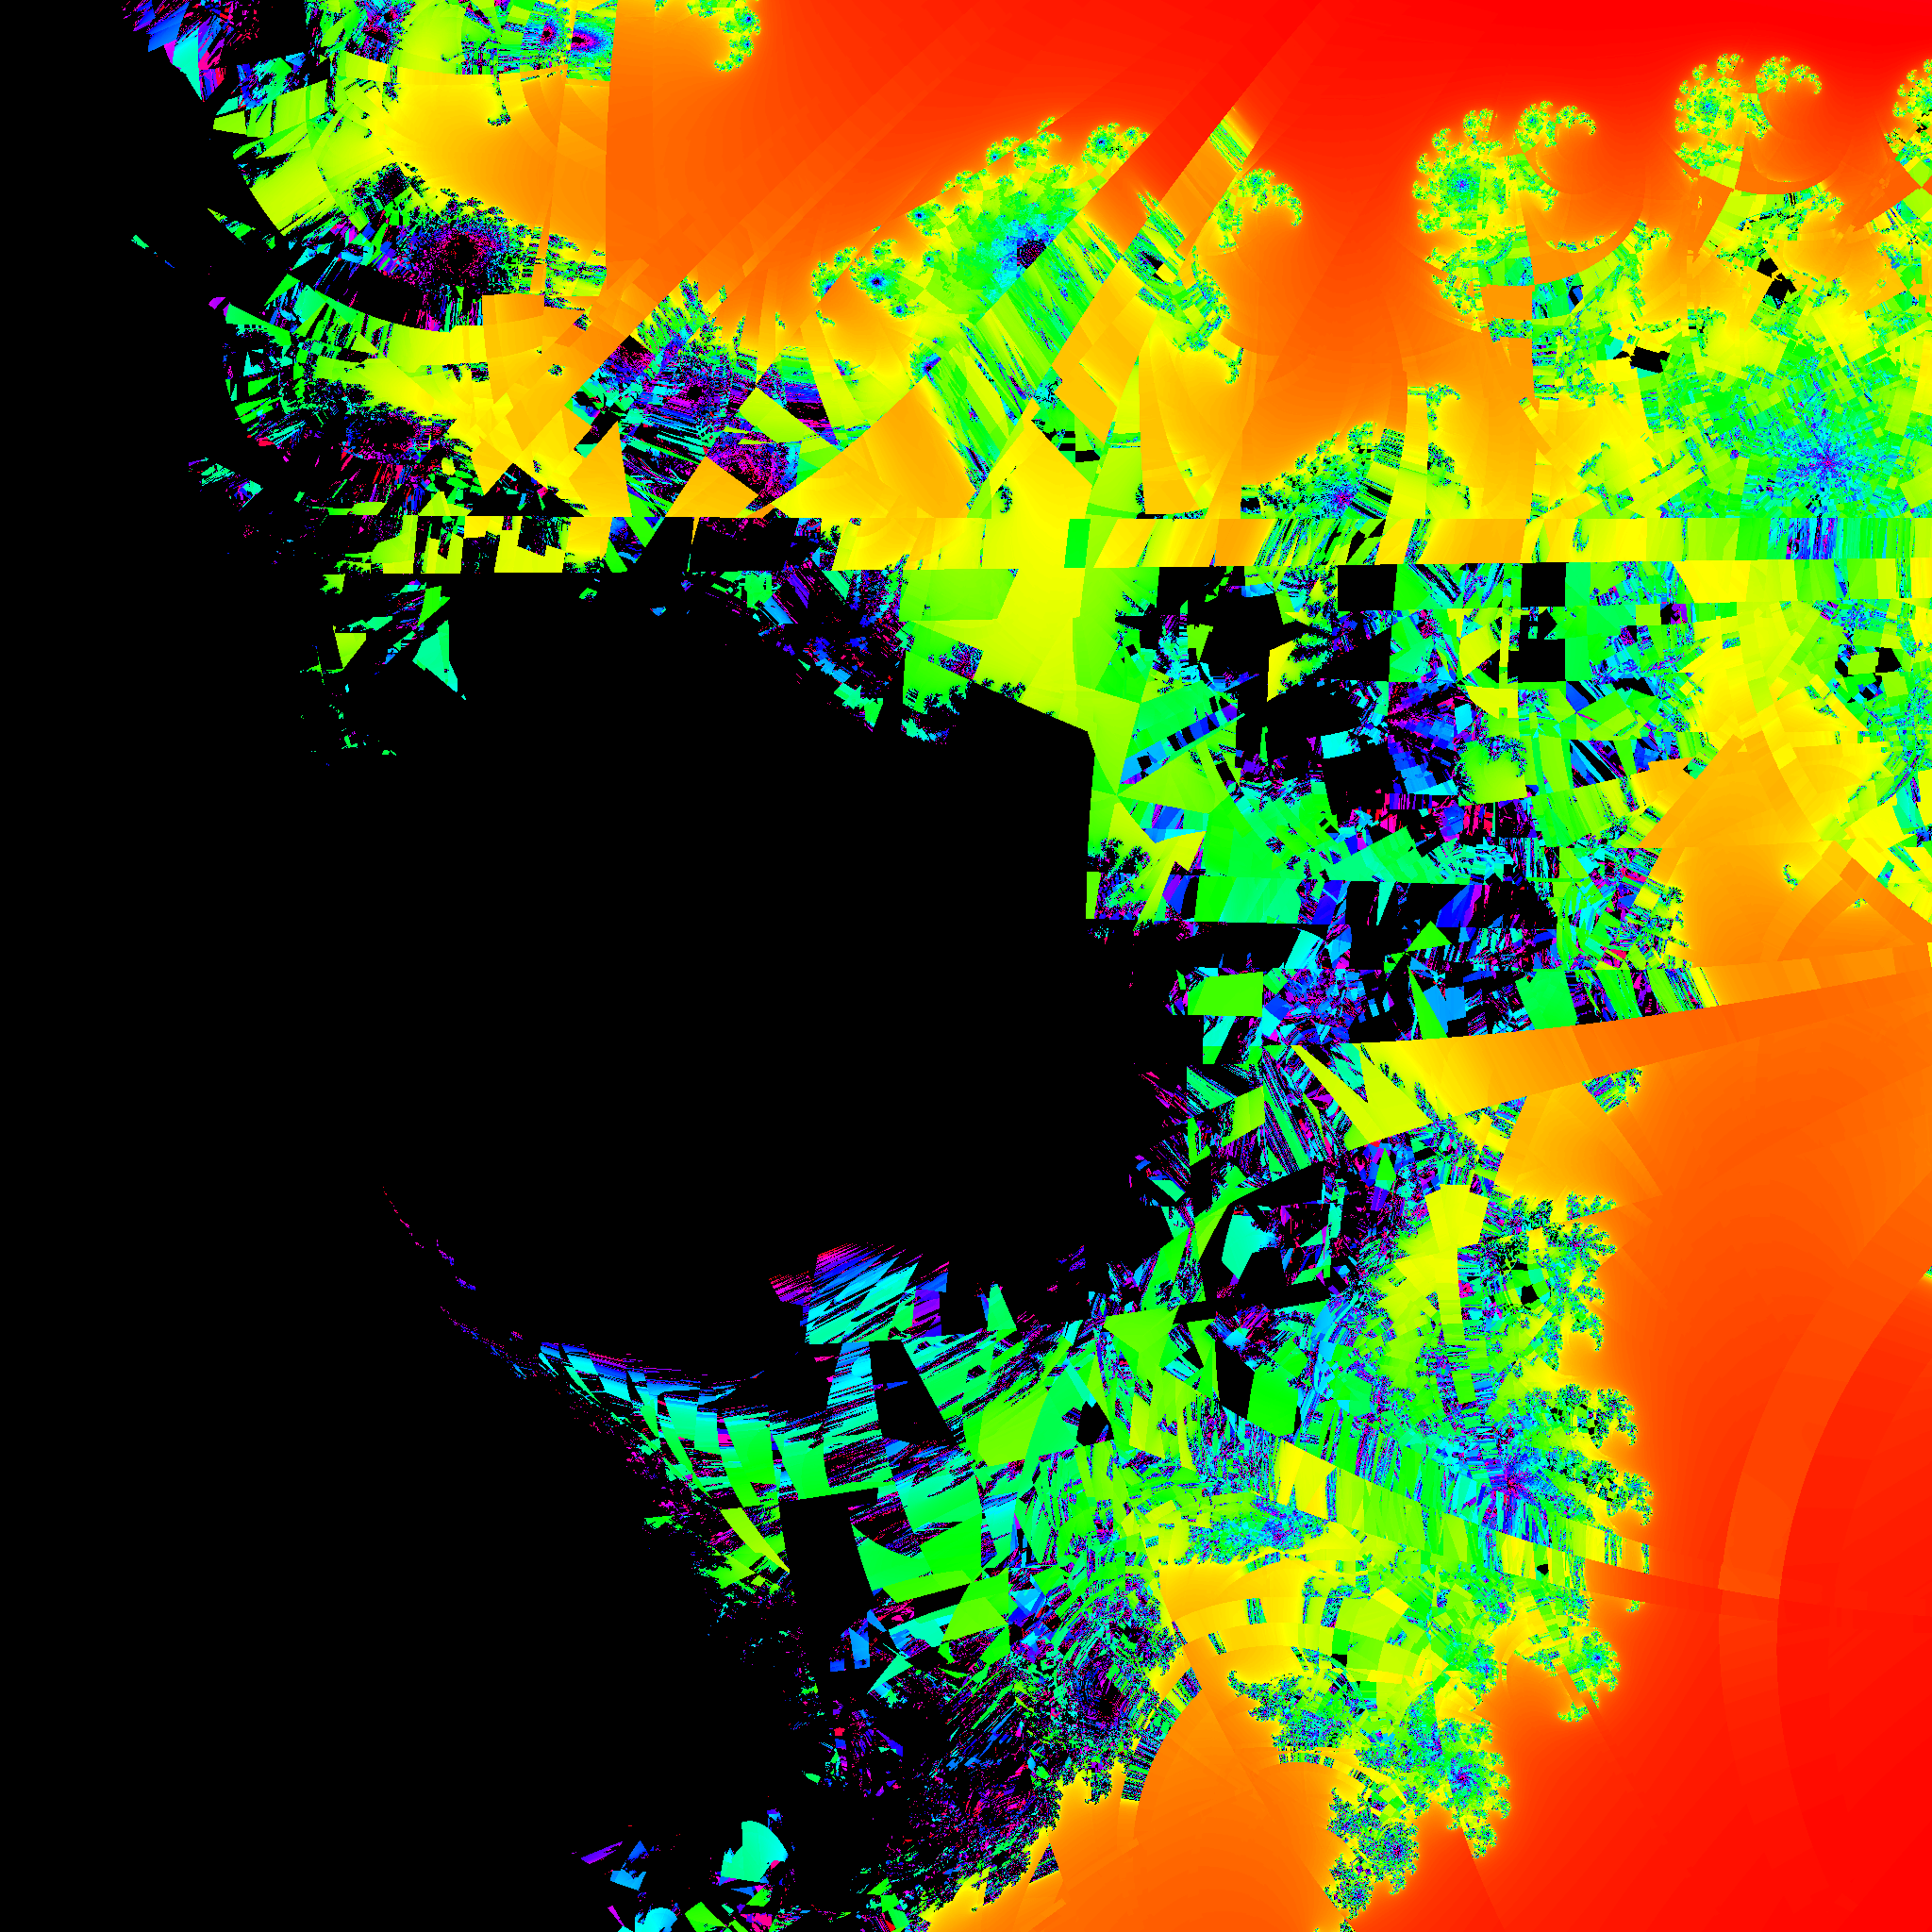
\includegraphics[width=0.8\textwidth]{images/teaser.png}
    \caption{We meant to do that.}
    \Description{A portion of the Mandelbrot fractal with some glitches.}
  \end{teaserfigure}


%%
%% This command processes the author and affiliation and title
%% information and builds the first part of the formatted document.
\maketitle

\section{Real Math\protect\footnotemark}
\footnotetext{Rational, not real. Rationality void where prohibited.}

\setcounter{subsection}{333984374}
\subsection{Feed me fractals}

In this paper, we investigate two fractals: the Mandelbrot set and a Newton
fractal. Both map a pixel coordinate $(x, y)$ into the complex plane as
a $c = x + yi$.

We evaluate the Mandelbrot set in the usual way:

\begin{align*} 
z_0     &= 0            \\
z_{n+1} &= {z_n}^2 + c
\end{align*}

\noindent up to an iteration limit ($n$).
Pixels that escape ($|z| \geq 2$) are given a
hue according to \cite{munafo:2023}. Pixels that do not escape are colored black.

We compute the Newton fractal on the polynomial $p(z) = z^3-1$:

\begin{align*}
z_0     &= c                        \\
z_{n+1} &= \frac{p(z_n)}{p'(z_n)}
\end{align*}

\noindent and plot whether $z$ reaches zero within a specified iteration limit.
Points that reach zero (within some threshold)
are grouped based on which zero of the function they are close to.
Pixels are colored by assigning each group a hue, and given a color value according to how many iterations it took to converge to zero.

\setcounter{subsection}{666015624}
\subsection{Exact computation via \texttt{BigRational}}

Since we’re rendering for a computer screen,
\footnote{Either our web interface, or the PDF version of this paper. If you're getting the print proceedings for SIGBOVIK, tough luck.}
we can (and do!) use exact inputs.

The raster grid (pixel grid) has integer locations, with $xres \times yres$ pixels.
We map each (integer) pixel location $(px,py)$ to a (rational) vector within the render window, centered at $(0,0)$

\begin{align*}
\hat{x} &= \frac{px}{xres} - \frac{1}{2} \\
\hat{y} &= \frac{1}{2} - \frac{py}{yres}
\end{align*}

We render a portion of the complex plane centered at $(\frac{x_c}{scale}, \frac{y_c}{scale})$, with equal width and height $\frac{size}{scale}$.
We constrain these to all be
rational numbers, which allows us to compute exact (rational) pixel coordinates:

\begin{align*}
x &= \hat{x} \times \frac{size}{scale} + \frac{x_c}{scale} \\
y &= \hat{y} \times \frac{size}{scale} + \frac{y
_c}{scale}
\end{align*}

We perform these computations using an arbitrary-precision rational number type, \texttt{num::BigRational} \cite{rust:num}.
\footnote{See also "BigMood: A novel format for arbitrary-precision emotional processing", to be published in SIGBOVIK 2025.}

In principle, we could also carry out the fractal computations exactly
using \texttt{BigRational}. The fractal formulae above require complex arithmetic,
which is simple,  plus some comparison operators ("greater than four" for Mandelbrot, "zeroish" for Newton).

When we tried to render the fractals using \texttt{BigRational}, though,
it reached a hard timeout (against the author's patience). Moreover, rationality has little place in an aesthetic evaluation such as this, so we stick
with finite-precision types.

\section{Unreal numbers}

Instead, we convert
\texttt{BigRational} values to various numeric formats,
approximating as closely as the format allows.
Some of the conversions might even be correct
(e.g. those we didn't write).

The formats we investigate are:

\begin{itemize}
  \item  \texttt{f32} and \texttt{f64}: IEEE 754 single- and double-precision floating-point formats\cite{cowlishaw2008standard}
  \item  \texttt{MaskedFloat<N,M>}, an IEEE 754 float with some exponent and/or mantissa bits removed
  \item  \texttt{IxFy}, fixed-point numeric formats \cite{fixedp, rust:fixed}
  \item  \texttt{P32}, \texttt{P16}, \texttt{P8}: 32/16/8-bit posits\texttrademark, an alternate float-like format\cite{posit}
\end{itemize}

\begin{figure*}
    \begin{subfigure}[bug]
        \centering
        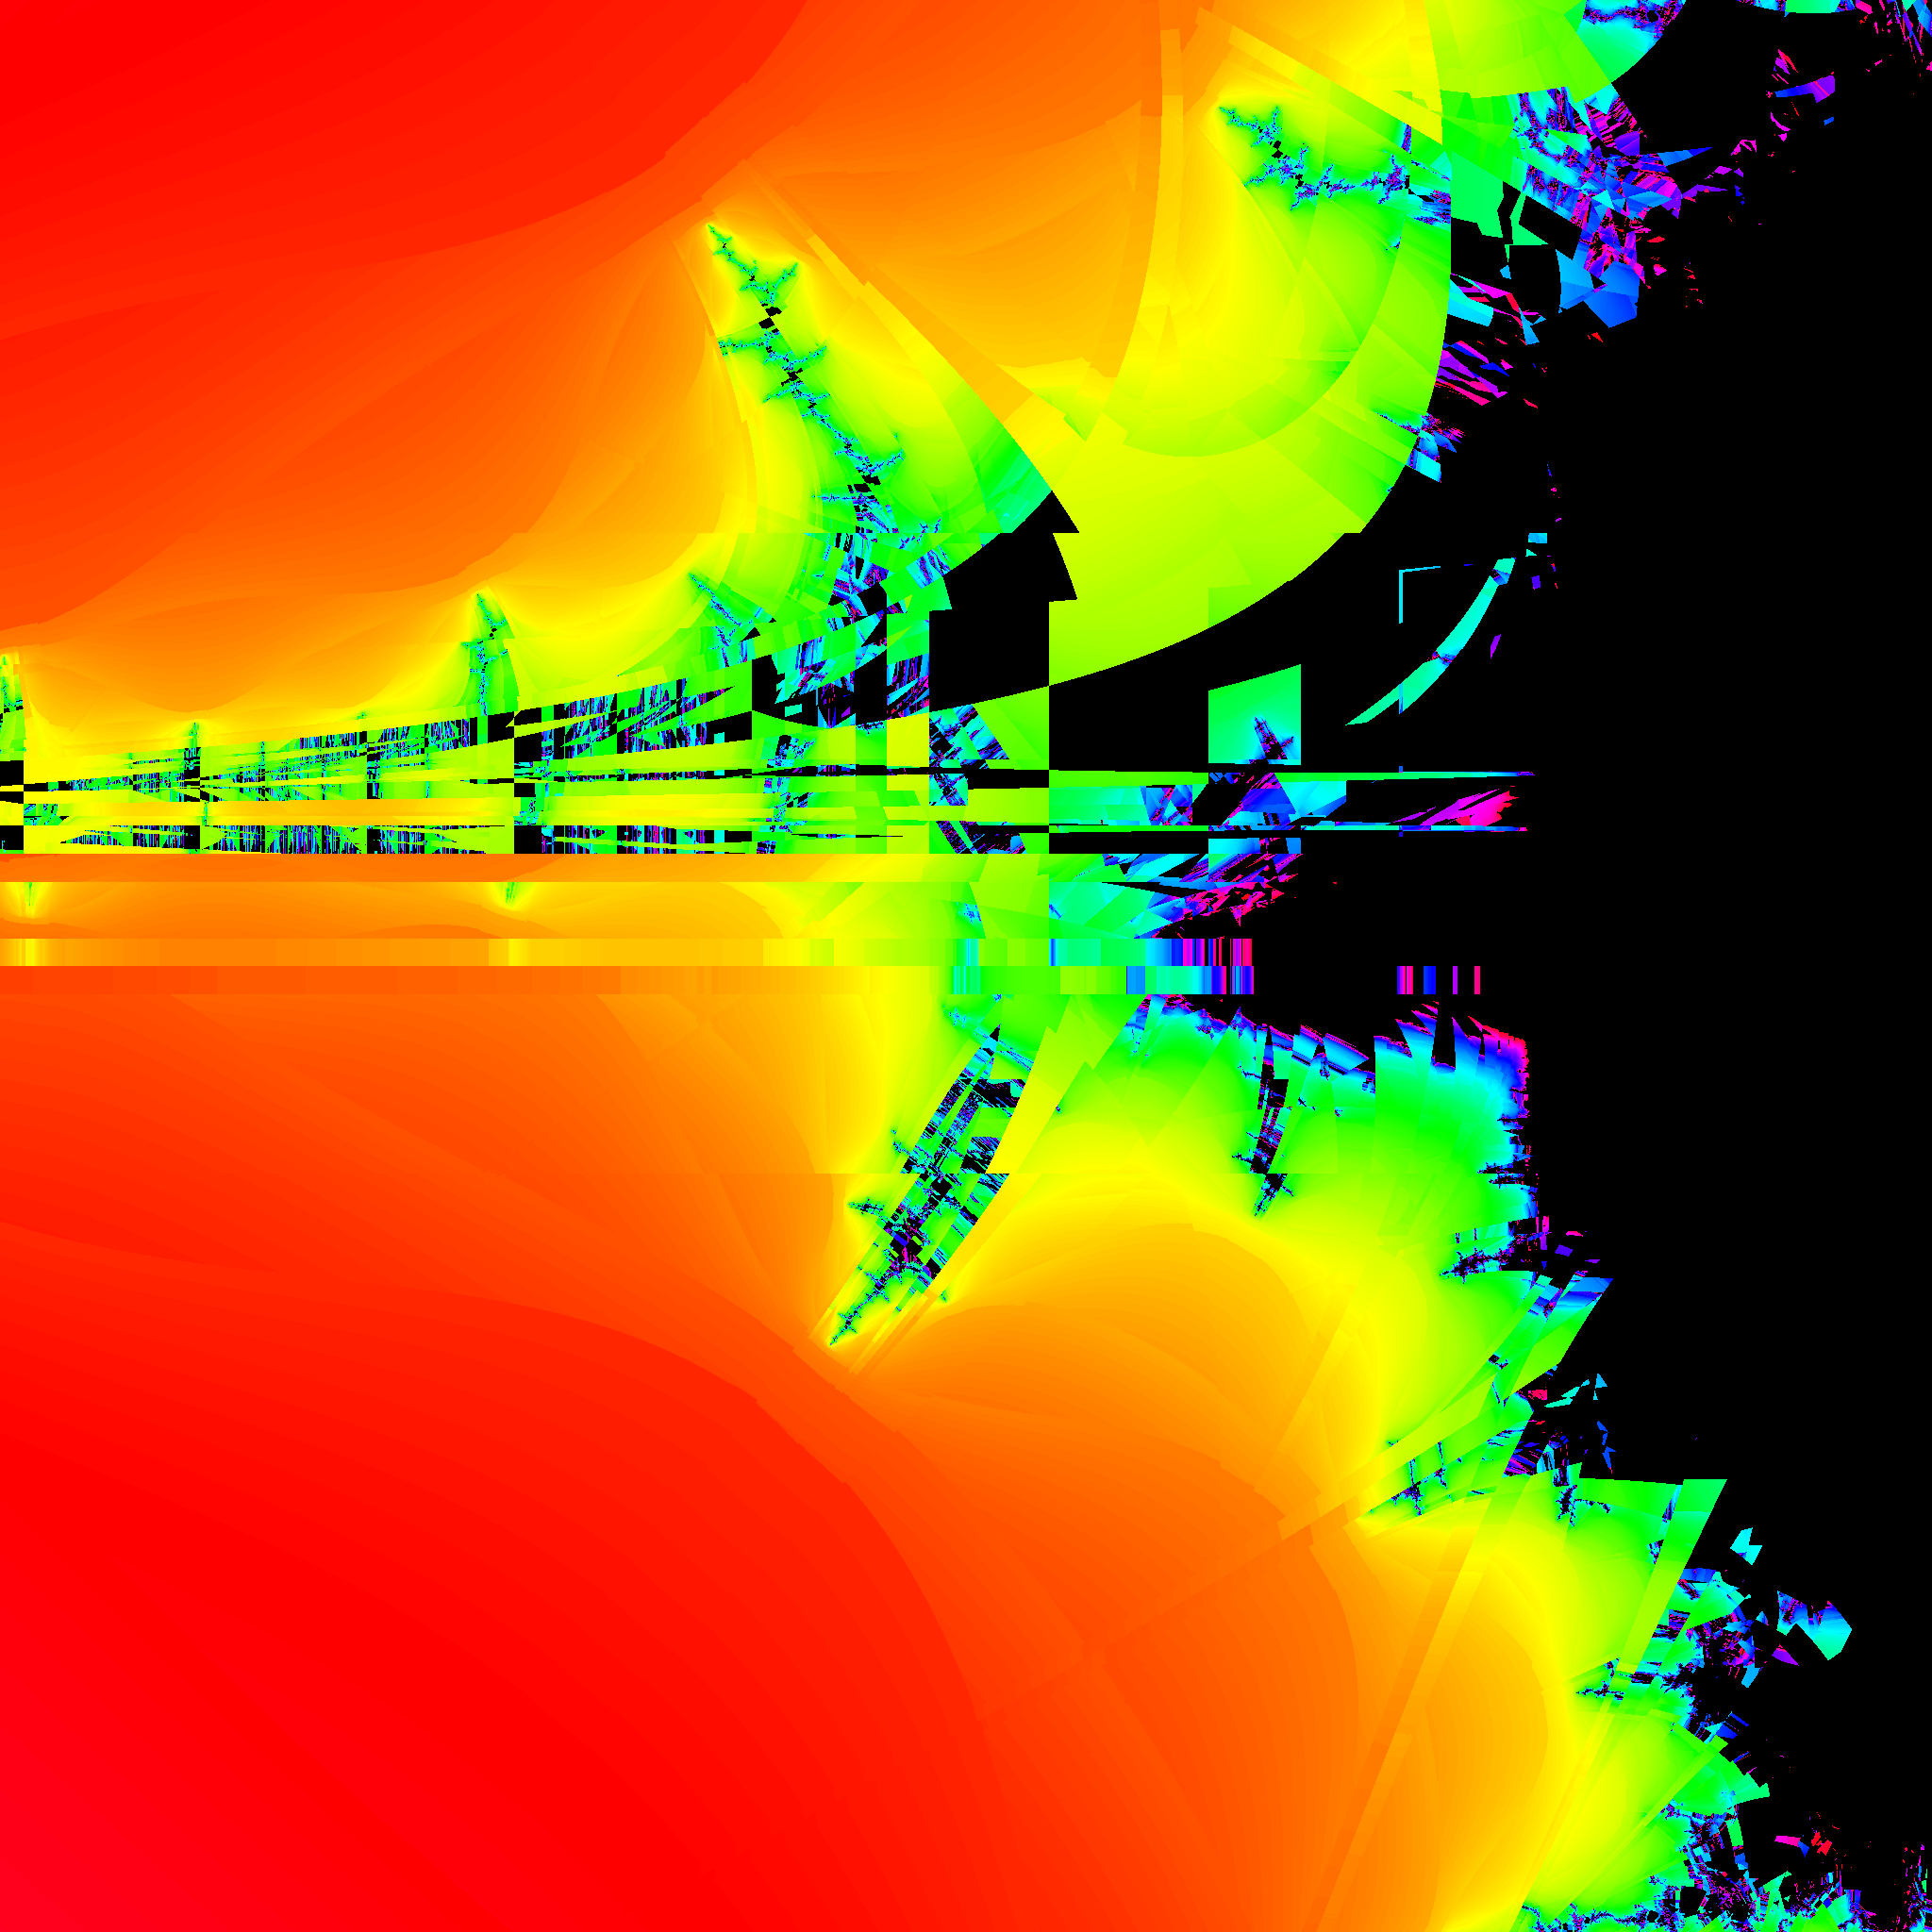
\includegraphics[width=0.48\linewidth]{images/0-mfbug/mf3-bugged.png}
    \end{subfigure}
    \quad
    \begin{subfigure}[no bug]
        \centering
        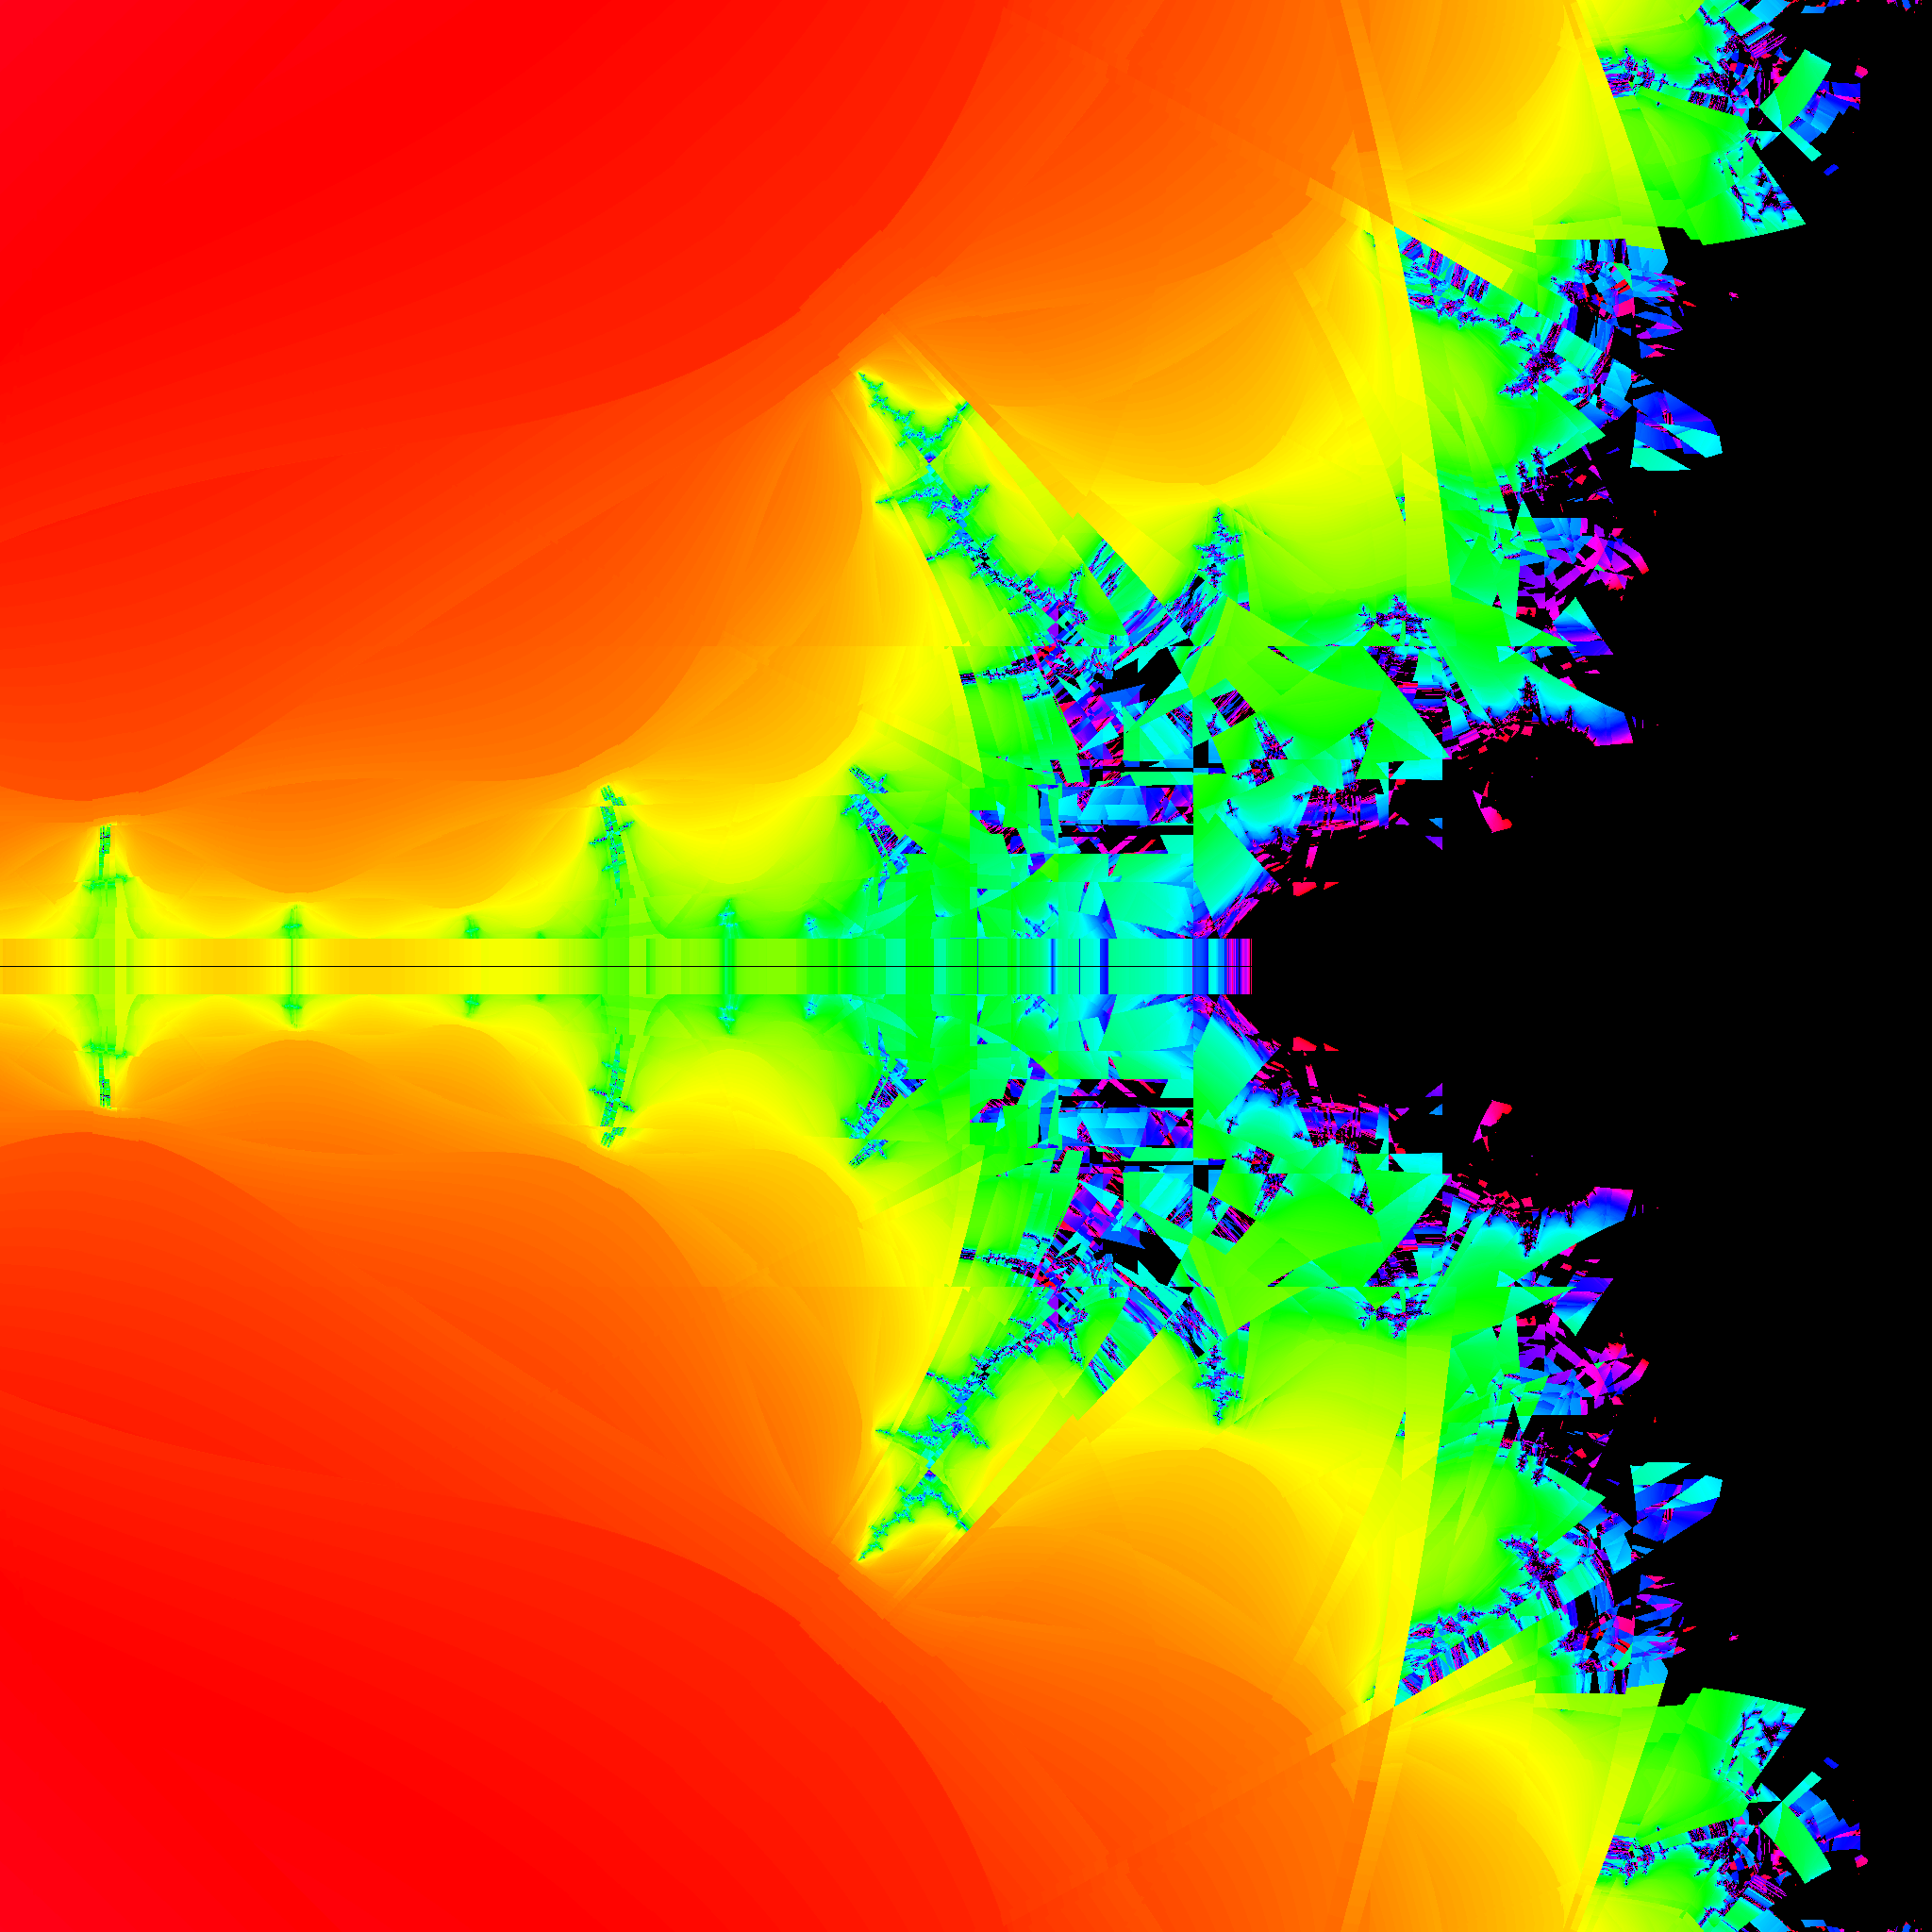
\includegraphics[width=0.48\linewidth]{images/0-mfbug/mf3-nobug.png}
    \end{subfigure}
    \caption{An asymmetric error in MaskedFloat}
    \label{fig:0-mfbug}
\end{figure*}

\setcounter{subsection}{124}
\subsection{MaskedFloat}

MaskedFloat isn’t yet a popular floating point type, but one we made up for this paper to try to create more interesting errors
than we were seeing with just IEEE \texttt{f64}.
It involves taking an \texttt{f64}, and masking off some of the bits, for our own amusement.

A normal \texttt{f64} consists of one bit of \textbf{s}ign, 11 bits of e\textbf{x}ponent, and then 52 \textbf{f}ractional bits, representing the value:

$$
(-1)^{s} \times (1.f_{51} f_{50} f_{48} ... f_0 ) \times 2^{x - 1023}
$$

If we want to experiment with what the world could be like if these were different (smaller) sizes, we can force some of those bits to one or zero.
For the fractional bits, this is easy, as they are an unsigned value--just setting the least-significant bits to zero gets rid of it.

For the exponential bits, this is more complicated. If we want to constrain the exponent to be effectively 4 bits (i.e., range from -7 to 8), we have to constrain the exponent value to be between 1016 and 1031).  Thankfully, we can do this with a bit of bit-twiddling. To make that easy to see, first, let’s see those values in binary:

\begin{align*}
1016 &= 0b01111111000 \\
1031 &= 0b10000000111
\end{align*}

So then, all we need to do is check if the most-significant fractional bit is set, then if it and any of bits [9:3] are set (i.e., it is greater than 1031), clamp down to 1031, and if the msb is not set, and any of bits [9:3] are also not set (i.e., less than 1016), clamp up to 1016.

This naive masking does have the side effect of re-introducing some of the problems near zero that IEEE had carefully removed when they added subnormals, as well as adding some more, unique problems. Since our goal in this paper is "shenanigans", that's great news for us.

The exponent has a special value, all-zeros, that is used along with an all-zero fraction to represent, unsurprisingly, zero. 
A naive exponent mask would turn that value instead into the smallest possible exponent (e.g., in the previous example, $2^{-1}$), which isn't quite accurate;  though that inaccuracy can be interesting, zero is a useful number for fractal computation, so we preserve this special-case behavior.

\setcounter{subsection}{24}
\subsection{Fixed-point}

We use the \texttt{fixed} Rust library \cite{rust:fixed} to perform fixed-point arithmetic.\footnote{We have especially high confidence in this library's numeric implementations. If any library has had all the bugs ironed out, it's \texttt{fixed}.}
The library offers a family of fixed-point formats specified as \texttt{IxFy}, with $x$ signed integer bits and $y$ fractional bits.

In this paper, we show a subset of the fixed-point formats we thought were coolest.

\setcounter{subsection}{374}
\subsection{Posits\texttrademark and quires}

For posits,\texttrademark we use the \texttt{softposit} Rust library\cite{rust:softposit}
and we implement conversion from \texttt{BigRational} via the associated quire
types. The quire formats are wider fixed-precision formats associated with posits\texttrademark.
For instance, the quire associated with the 32-bit posit\texttrademark is 512 bits wide, with a precision
of $2^{-240}$ -- roughly equivalent to an \texttt{I241F240} fixed-point.

\setcounter{subsection}{4}
\subsection{Sources of distortion}

When rendering fractals, distortion, like inspiration, can come from anywhere.

\setcounter{subsubsection}{19921874}
\subsubsection{Bugs}

When implementing the MaskedFloat type, the authors originally did not properly account for the special case around zero, and instead represented it as the smallest possible positive number. This resulted in strange, but pretty neat looking, asymmetrical error,
depicted in Figure \ref{fig:0-mfbug}.

% /mandelbrot/render/MaskedFloat%3C3,50%3E?x=-21&y=0&window=8&scale=15&res=2048&iters=40
% with bug and without bug

\setcounter{subsubsection}{400390624}
\subsubsection{Scale}

The Mandelbrot and Newton fractals both exhibit self-similarity, repeating themselves at
various scales. However, not all of the formats sampled can operate at multiple scales:
all of them have some scaling limits, but some are more limited than others.

This is most obvious when dealing with fixed-point formats. \texttt{I11F5}, for instance,
can only represent 128 distinct values in the range $|z| < 2$ - where the Mandelbrot set lives.
That's fewer than the pixels used to render these images -- hence, pixelation, as shown in Figure \ref{fig:1-nozoom}.

The nature and pattern of the pixelation depends on the format used, as shown in Figure \ref{fig:1-zoom}.
In a region of size $\frac{2}{3}$ centered on $\frac{-4}{3} + 0i$, the \texttt{P8} and \texttt{I11F5}
formats show different aesthetic qualities. P8 (depicted) and floating-point stretch into rectangles,
as is apparent when far from $x=y$; while fixed-point gives the appearance of overlapping tiles.

% This is just the "mandelbrot" default page
\begin{figure*}
    \begin{subfigure}[f32]
        \centering
        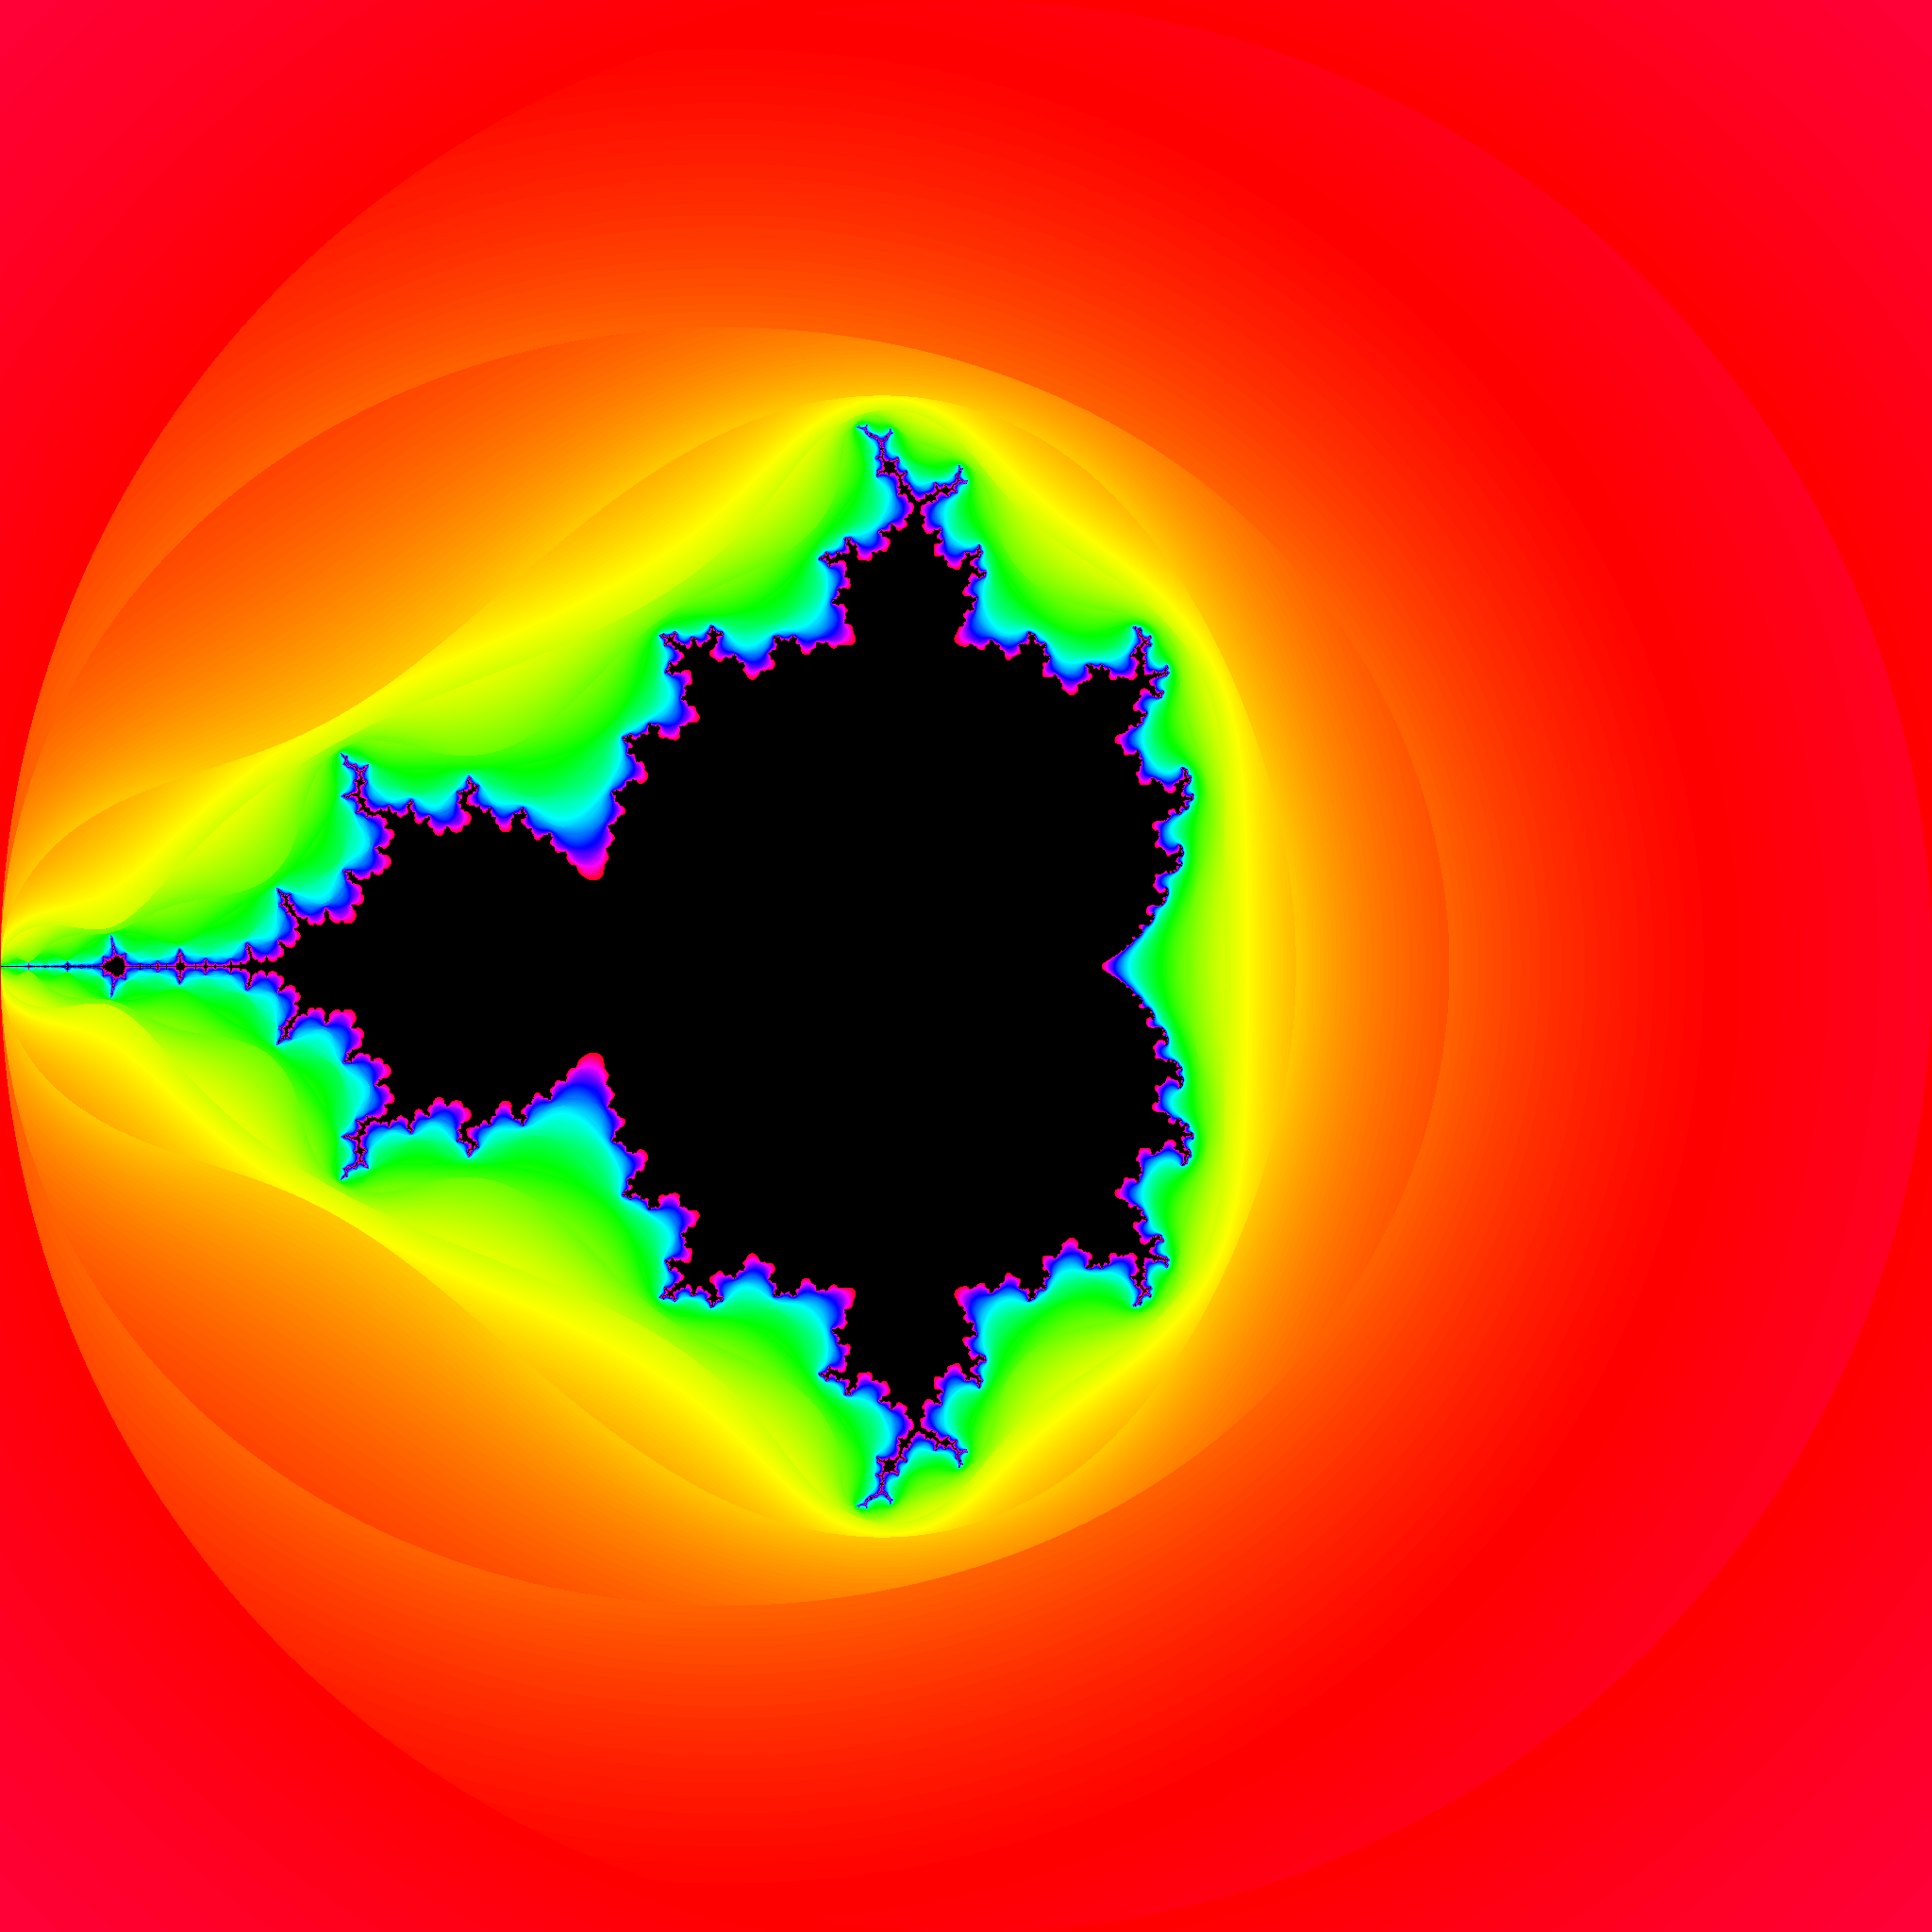
\includegraphics[width=0.4\linewidth]{images/1-nozoom/f32.png}
    \end{subfigure}
    \quad
    \begin{subfigure}[I11F5]
        \centering
        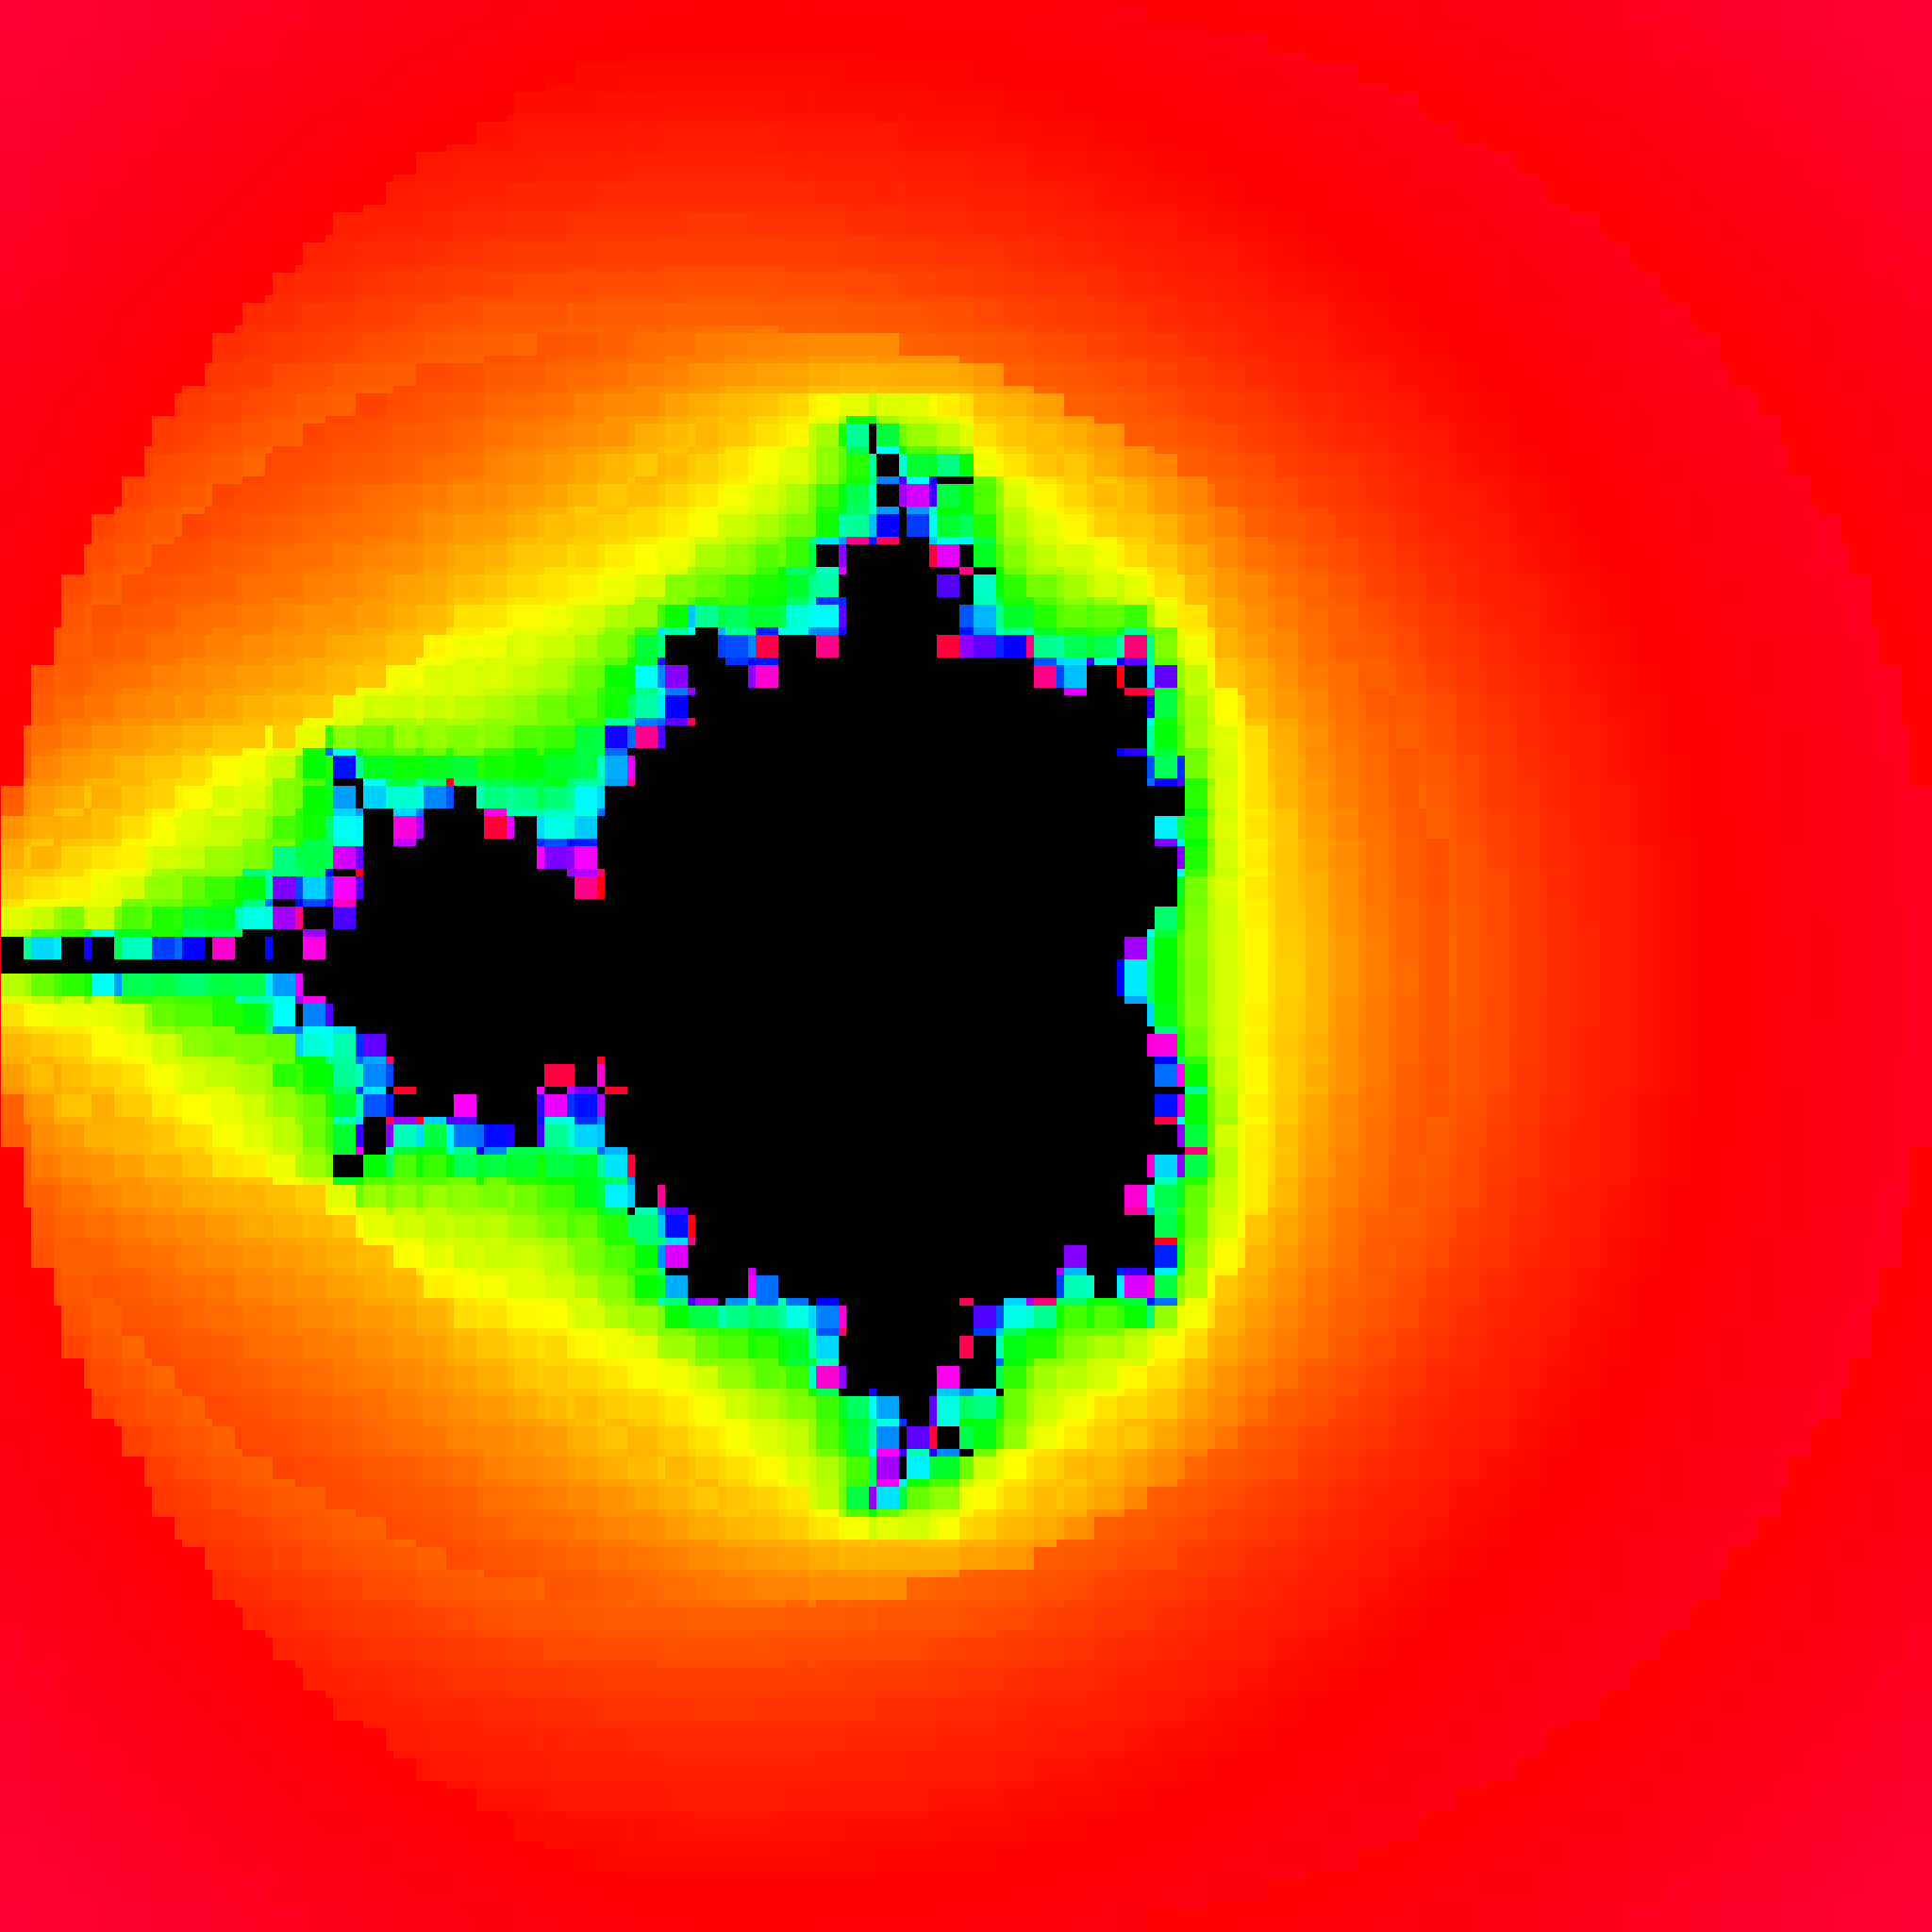
\includegraphics[width=0.4\linewidth]{images/1-nozoom/I11F5.png}
    \end{subfigure}
    \caption{f32 and I11F5, -2 to 2}
    \label{fig:1-nozoom}
\end{figure*}

% /mandelbrot/?x=-4&y=0&window=2&scale=3&res=512&iters=16
\begin{figure}
    \begin{subfigure}[P8]
        \centering
        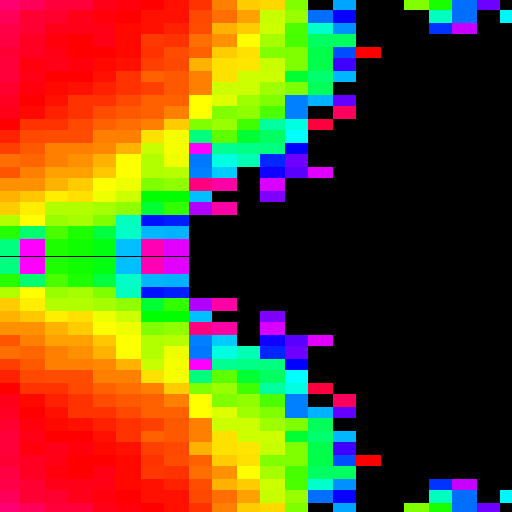
\includegraphics[width=0.45\linewidth]{images/1-nozoom/P8-zoom.png}
    \end{subfigure}
    \quad
    \begin{subfigure}[I11F5]
        \centering
        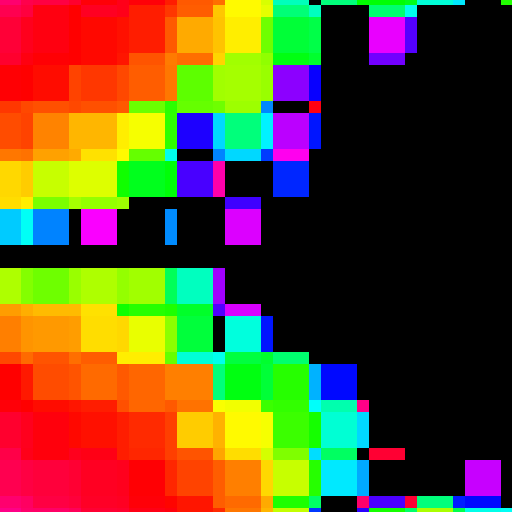
\includegraphics[width=0.45\linewidth]{images/1-nozoom/I11F5-zoom.png}
    \end{subfigure}
    \caption{Two pixelations near $\frac{-4}{3}$}
    \label{fig:1-zoom}
\end{figure}

\begin{figure}
    \centering
    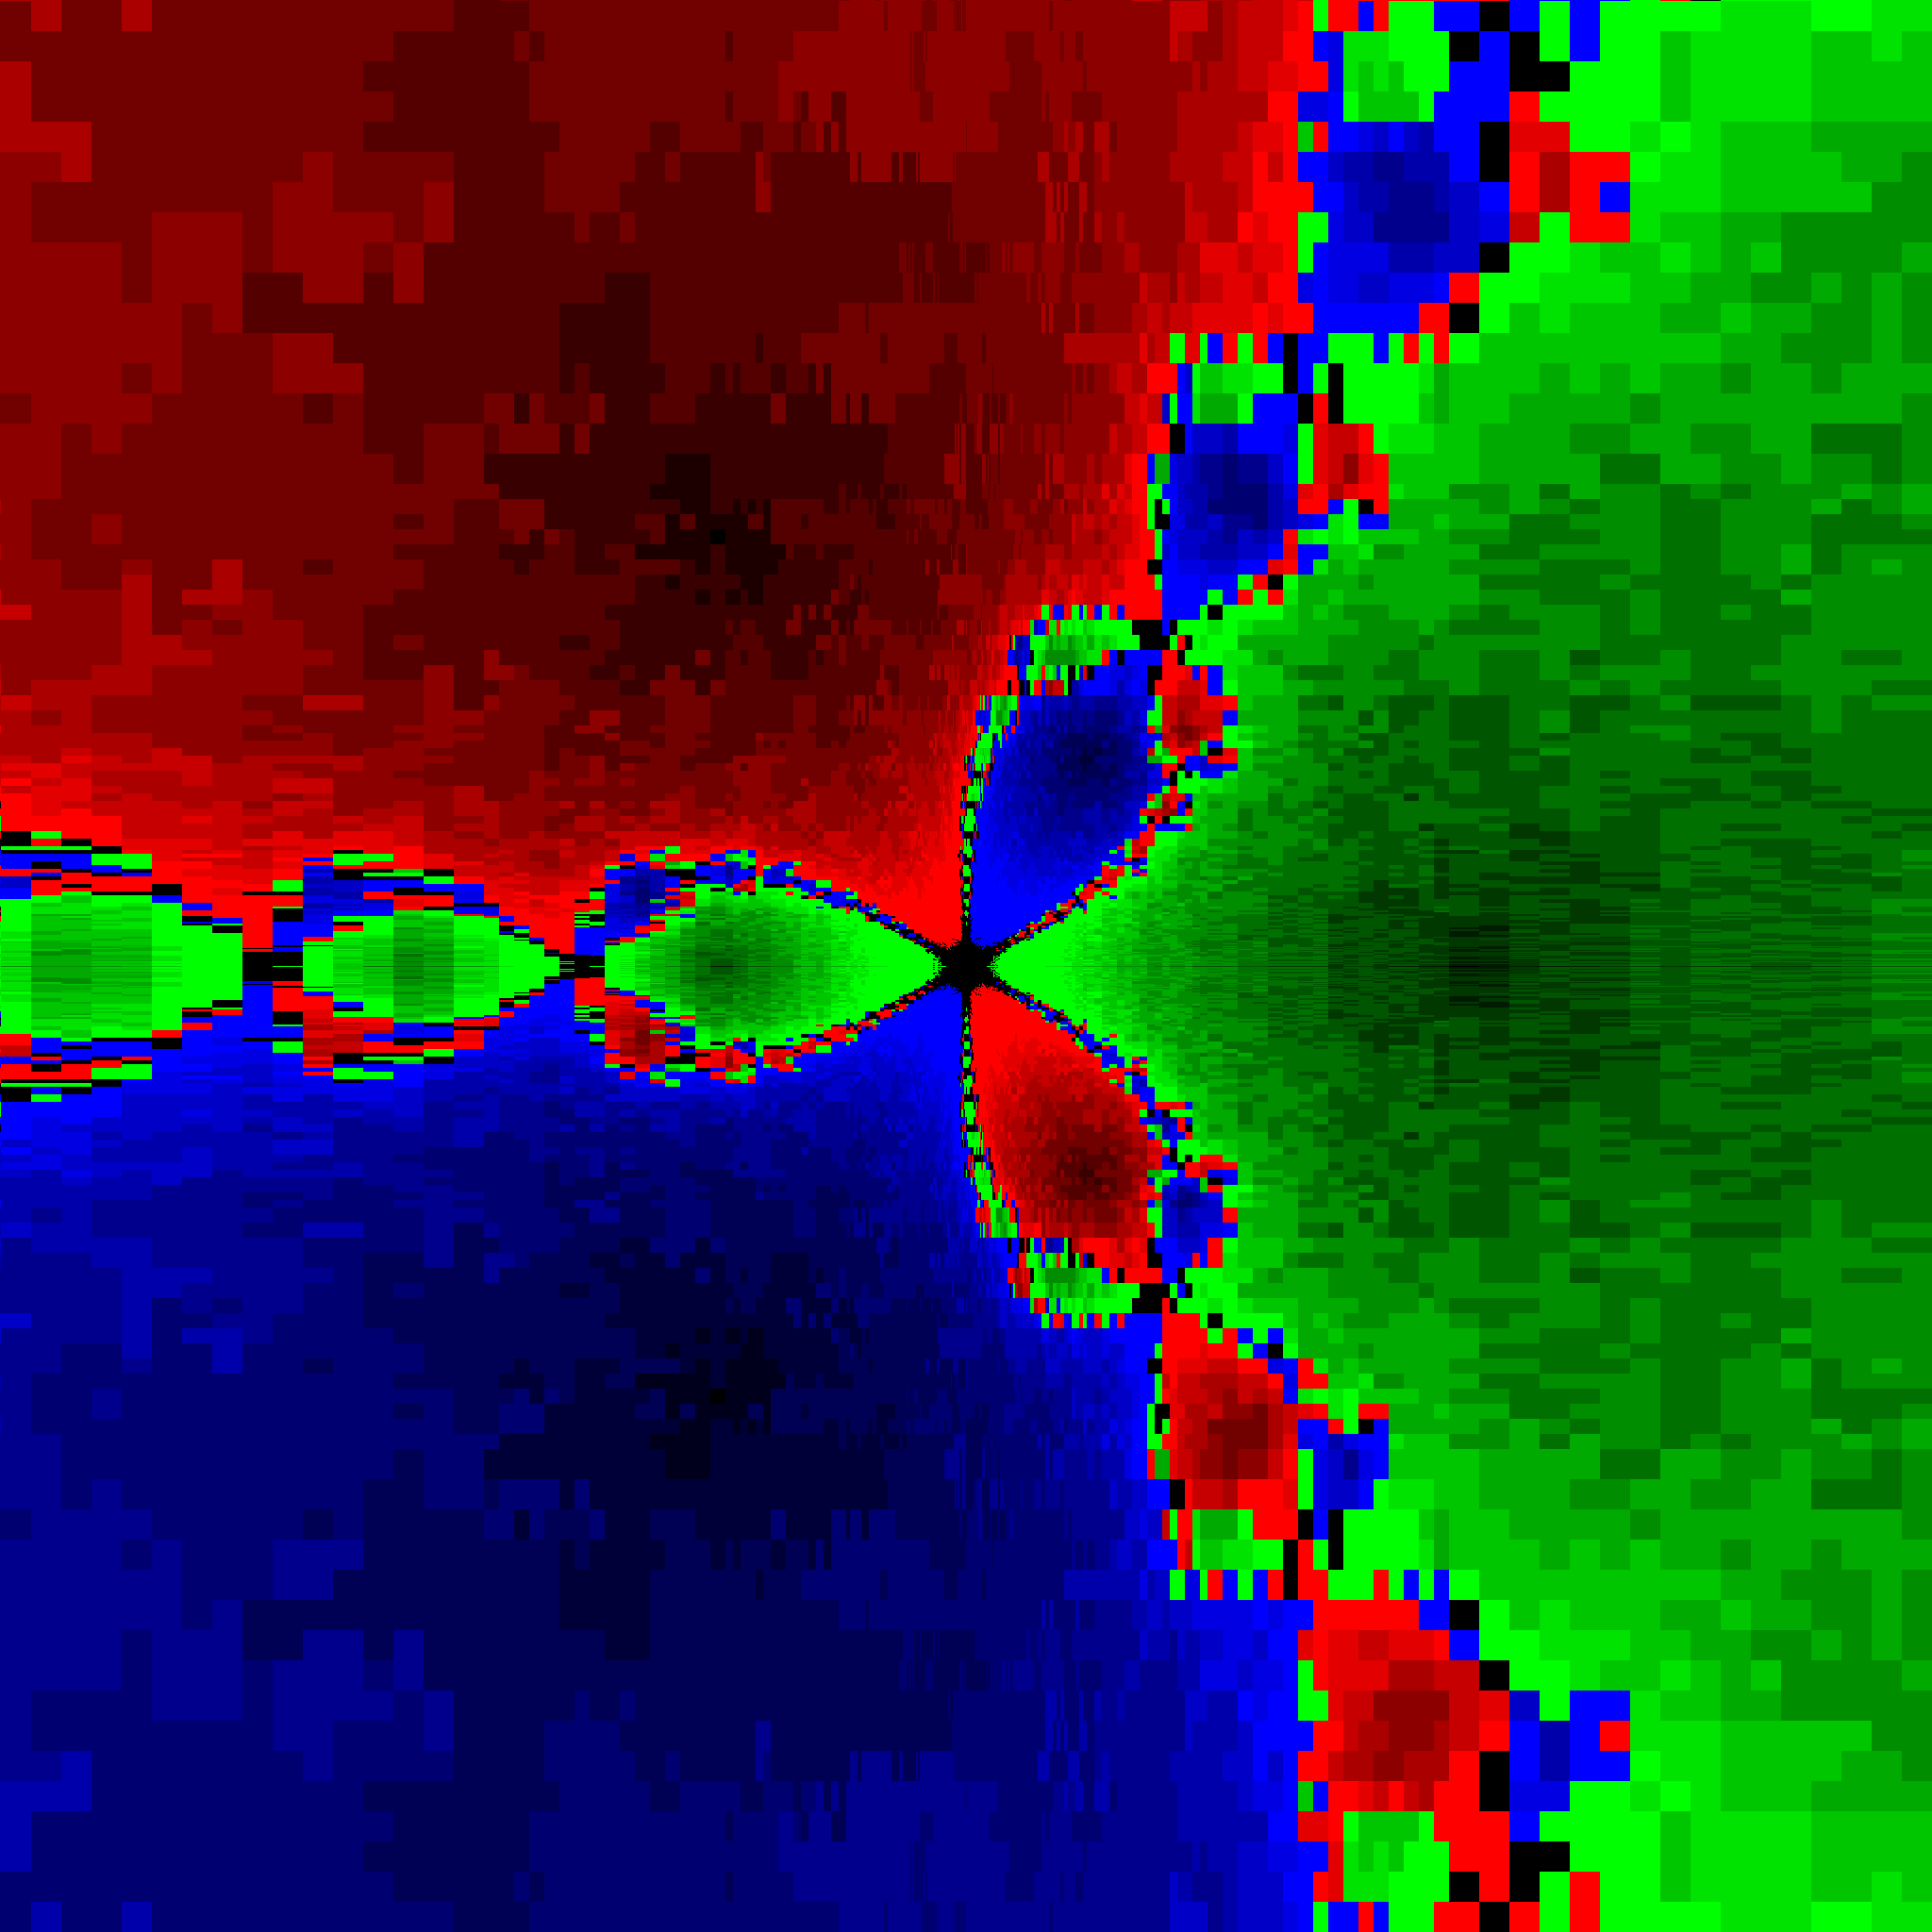
\includegraphics[width=0.9\linewidth]{images/1-mantissa/mf63.png}
    \caption{MaskedFloat<6,3>}
    \label{fig:1-mantissa}
\end{figure}

\setcounter{subsubsection}{599609374}
\subsubsection{Precision error}

It's possible to preserve dynamic range (see section \ref{hdr}) but lose precision,
as in \texttt{MaskedFloat<6,3>}: it has 6 bits of exponent (scale), but only 4 bits at
any given scale.

%% /mandelbrot/?x=-32751&y=-38190&window=4096&scale=59049&res=2048&iters=40
\begin{figure*}
    \begin{subfigure}[f64]
        \centering
        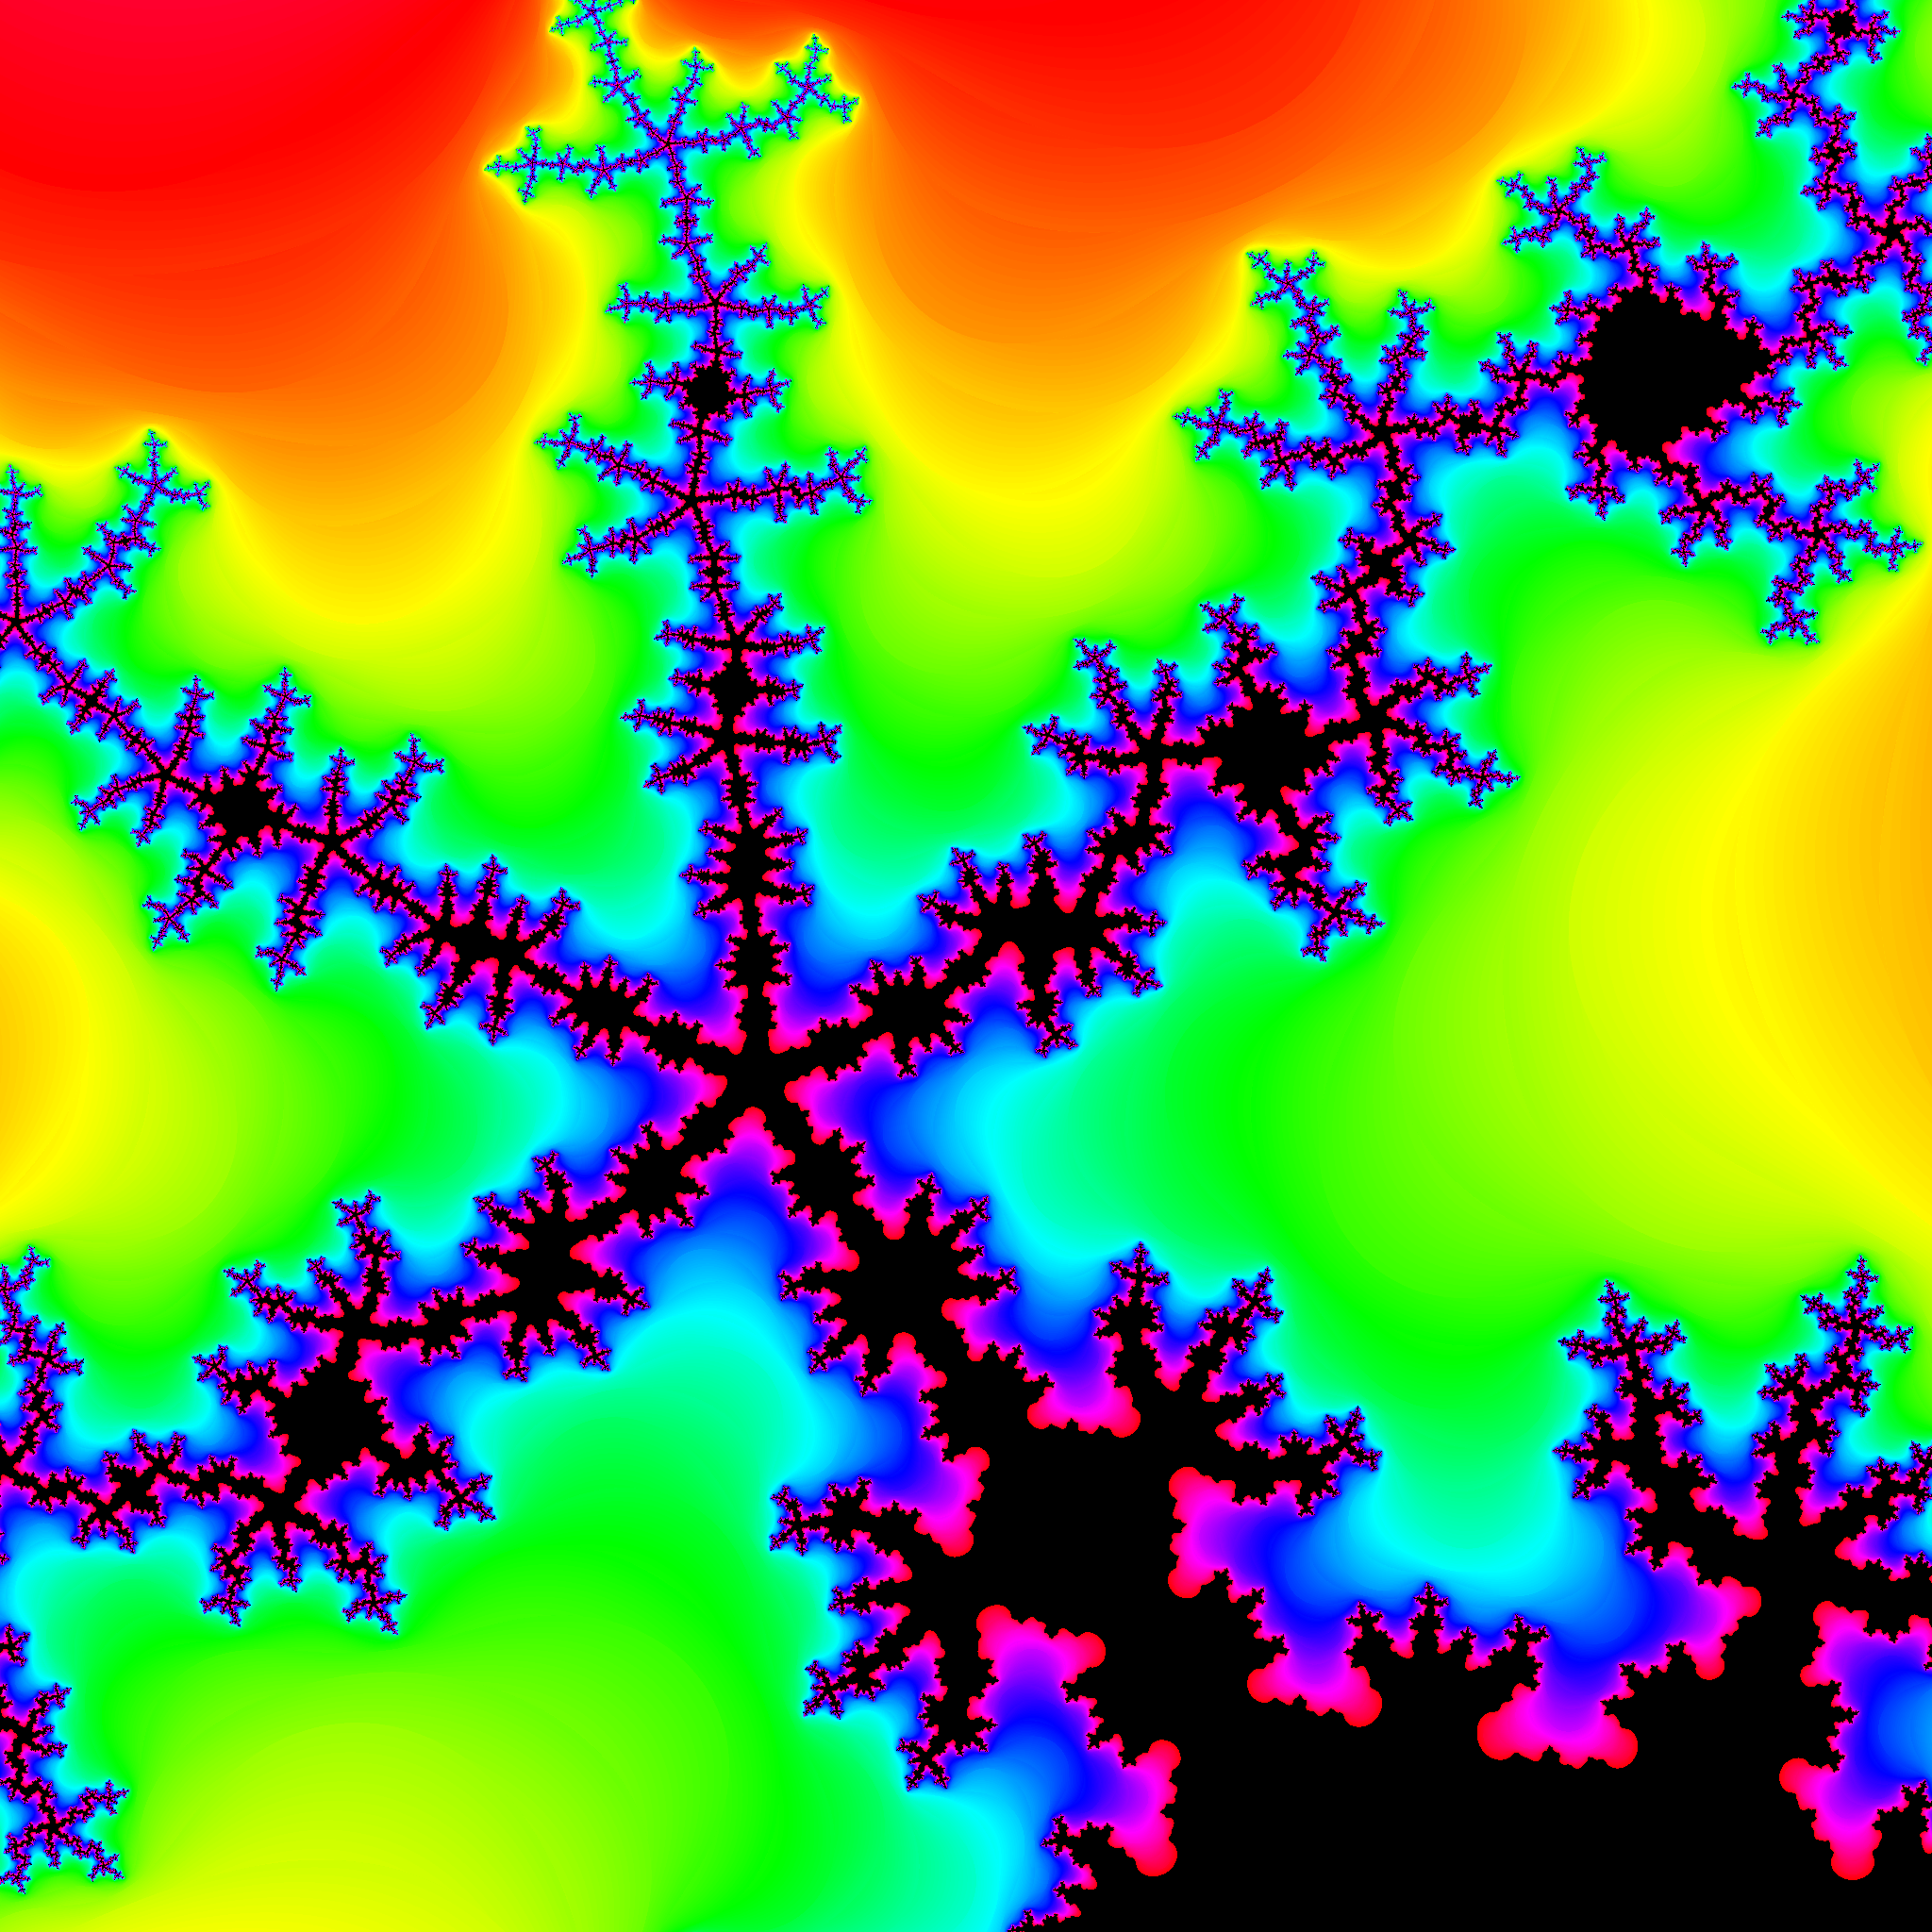
\includegraphics[width=0.35\linewidth]{images/3-masked_curves/curves_f64.png}
    \end{subfigure}
    \quad
    \begin{subfigure}[MaskedFloat]
        \centering
        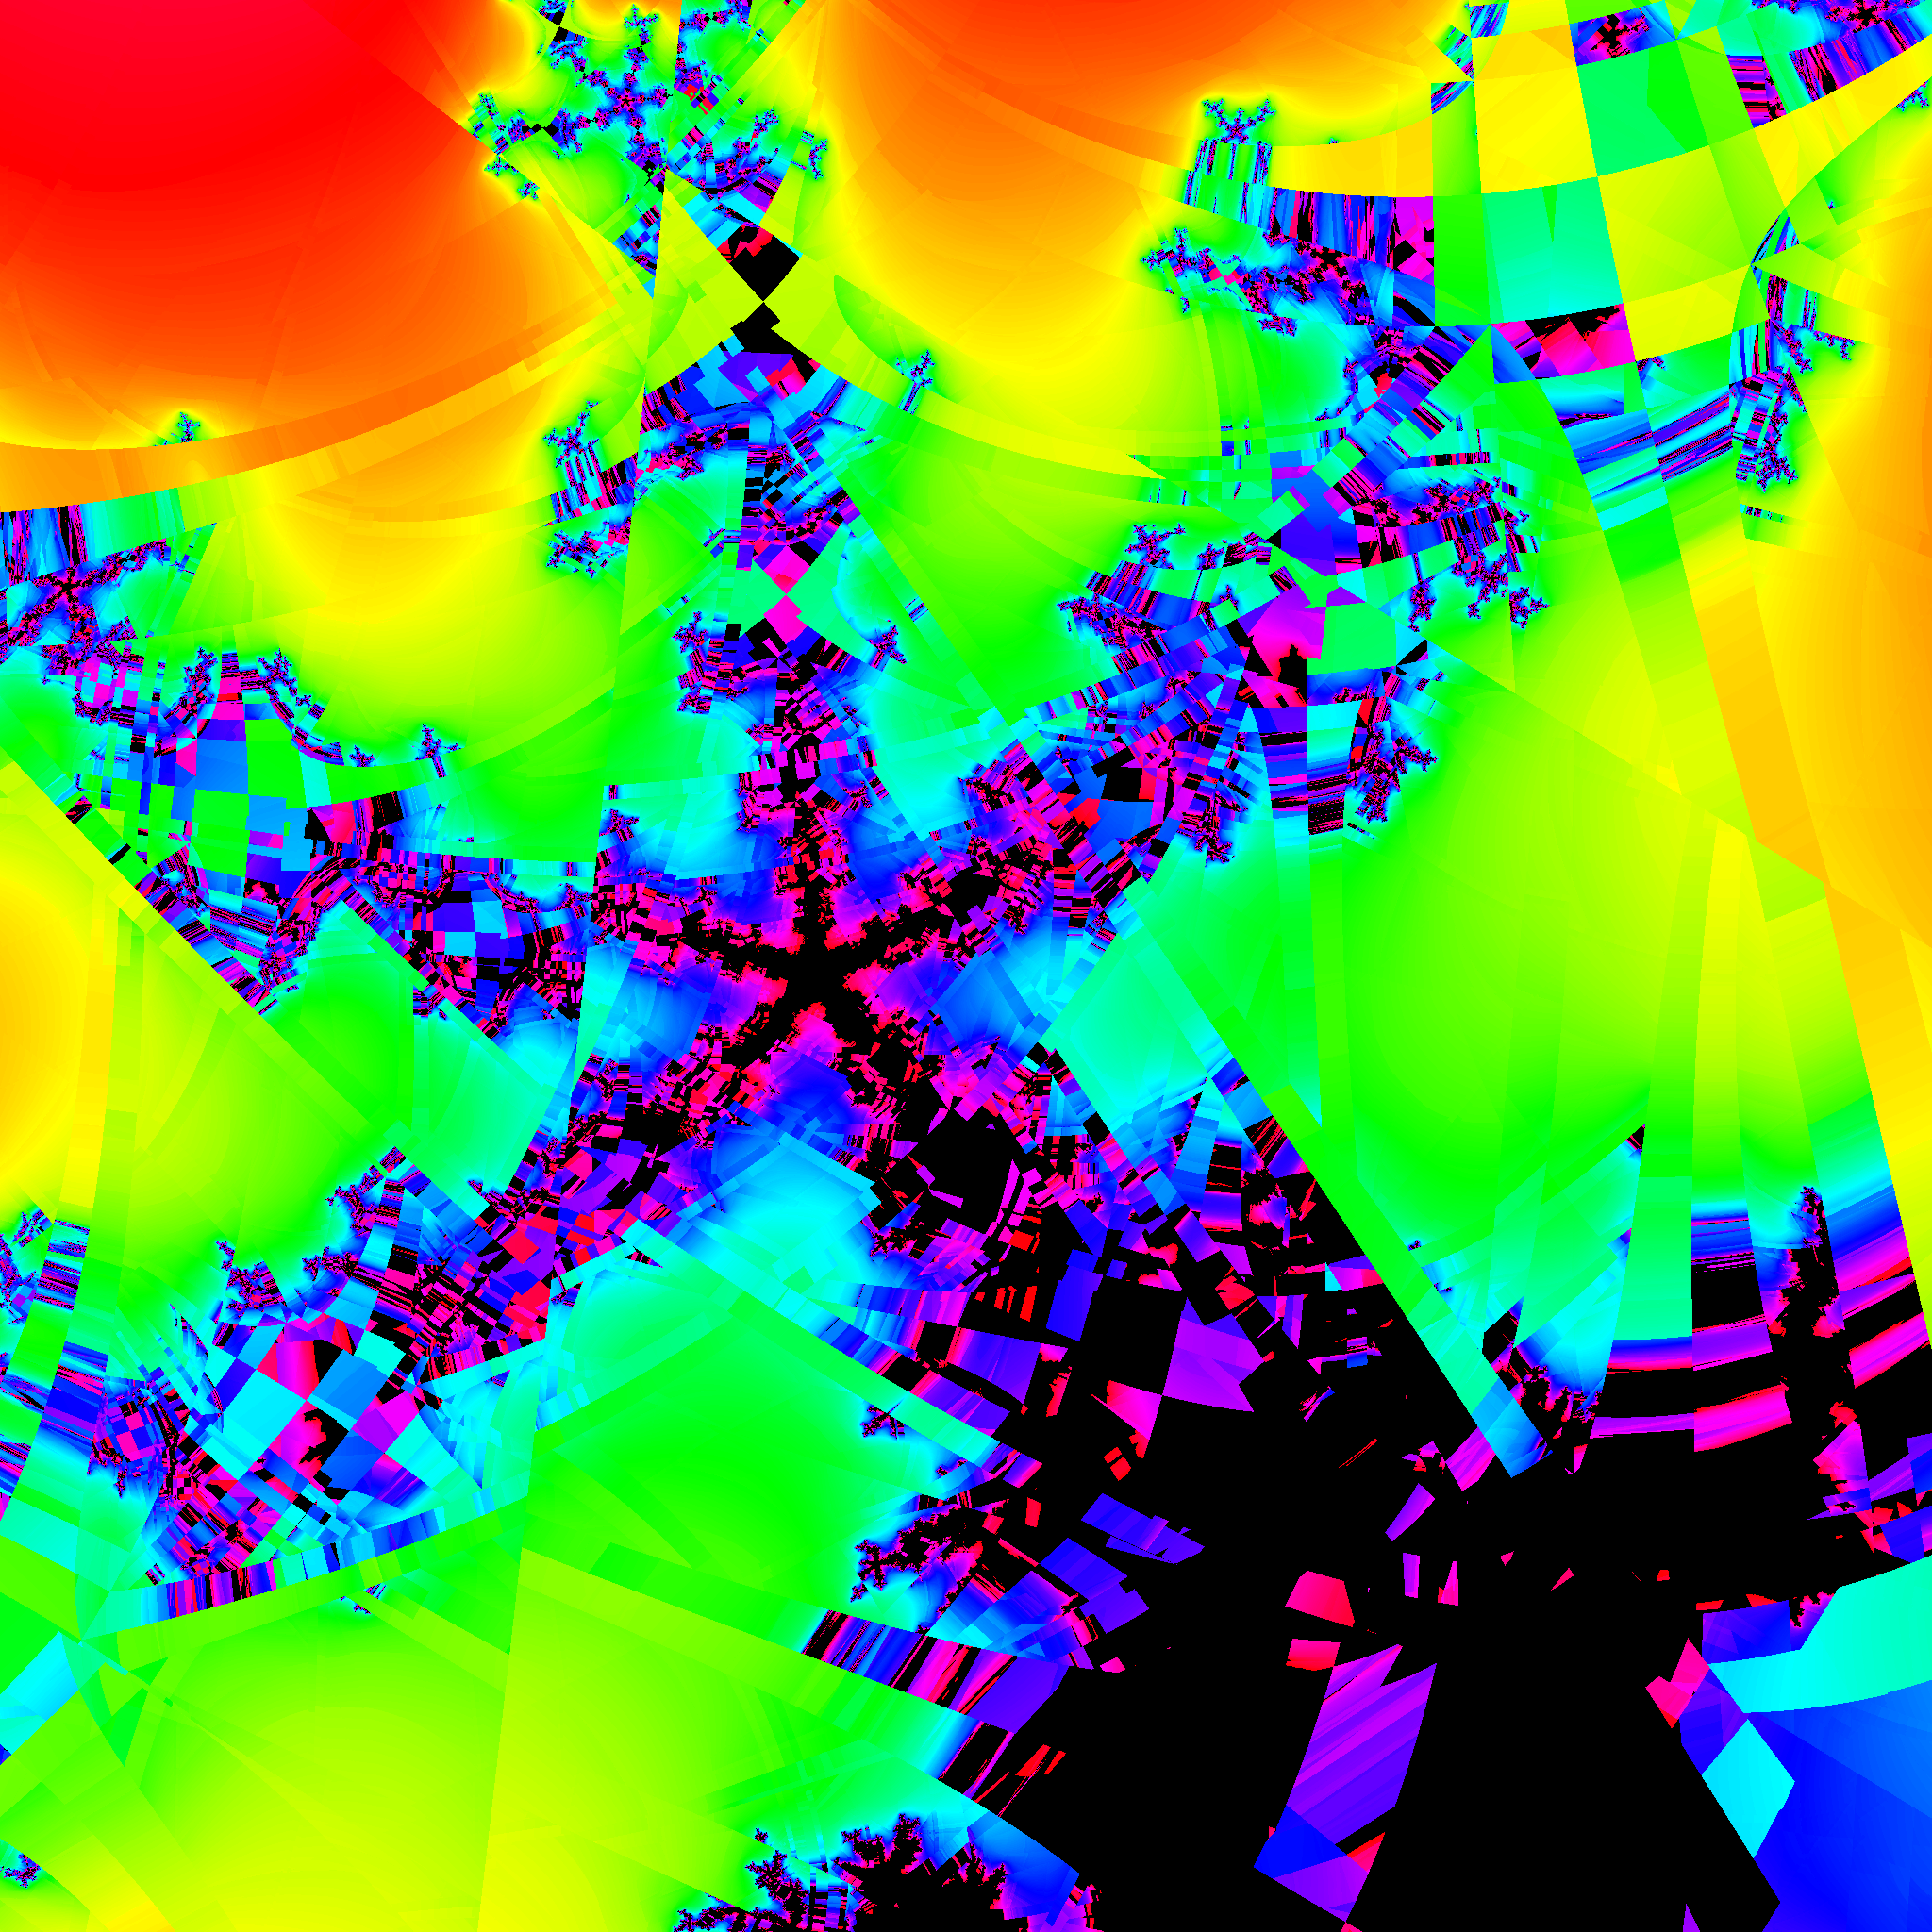
\includegraphics[width=0.35\linewidth]{images/3-masked_curves/curves_MaskedFloat_3_50.png}
    \end{subfigure}
    \quad
    \caption{Exponent errors in MaskedFloat<3,50>}
    \label{fig:3-curves}
\end{figure*}

%% http://172.23.199.99:3000/newton/?x=0&y=0&window=4&scale=1&res=512&iters=64
\begin{figure*}
    \begin{subfigure}[f64]
        \centering
        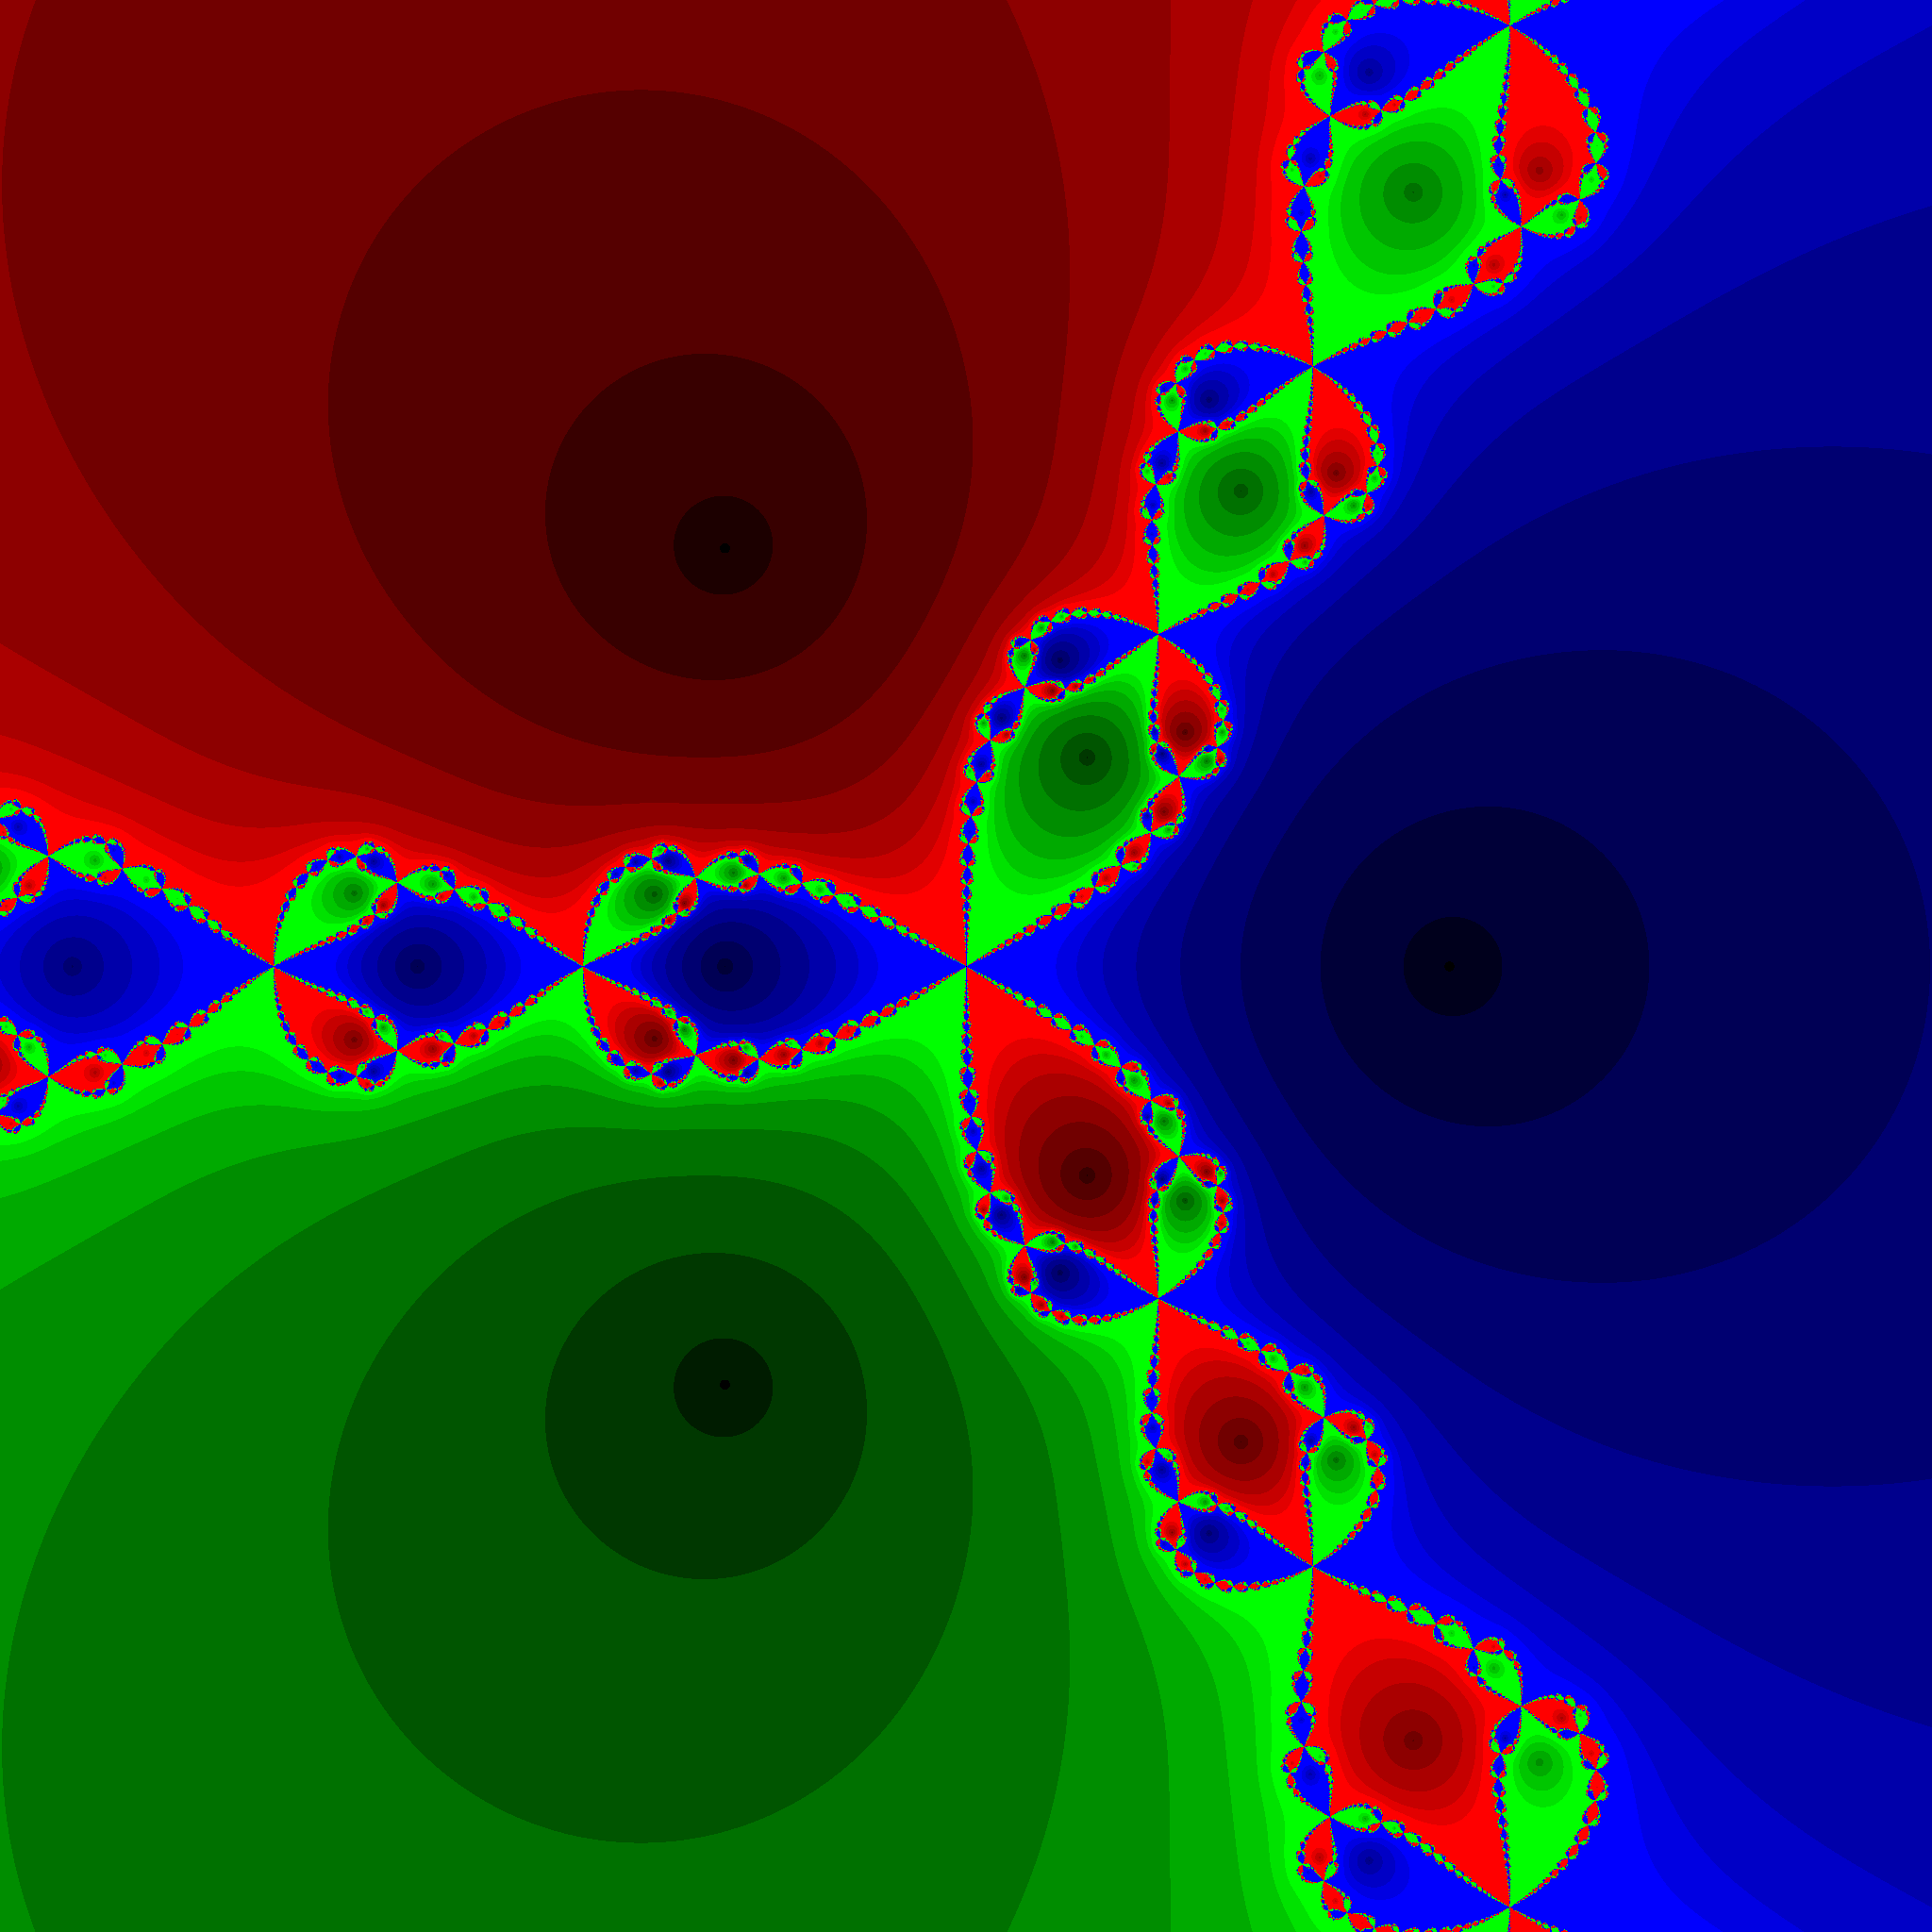
\includegraphics[width=0.35\linewidth]{images/fixed_newton/newton_f64.png}
    \end{subfigure}
    \quad
    \begin{subfigure}[I22F10]
        \centering
        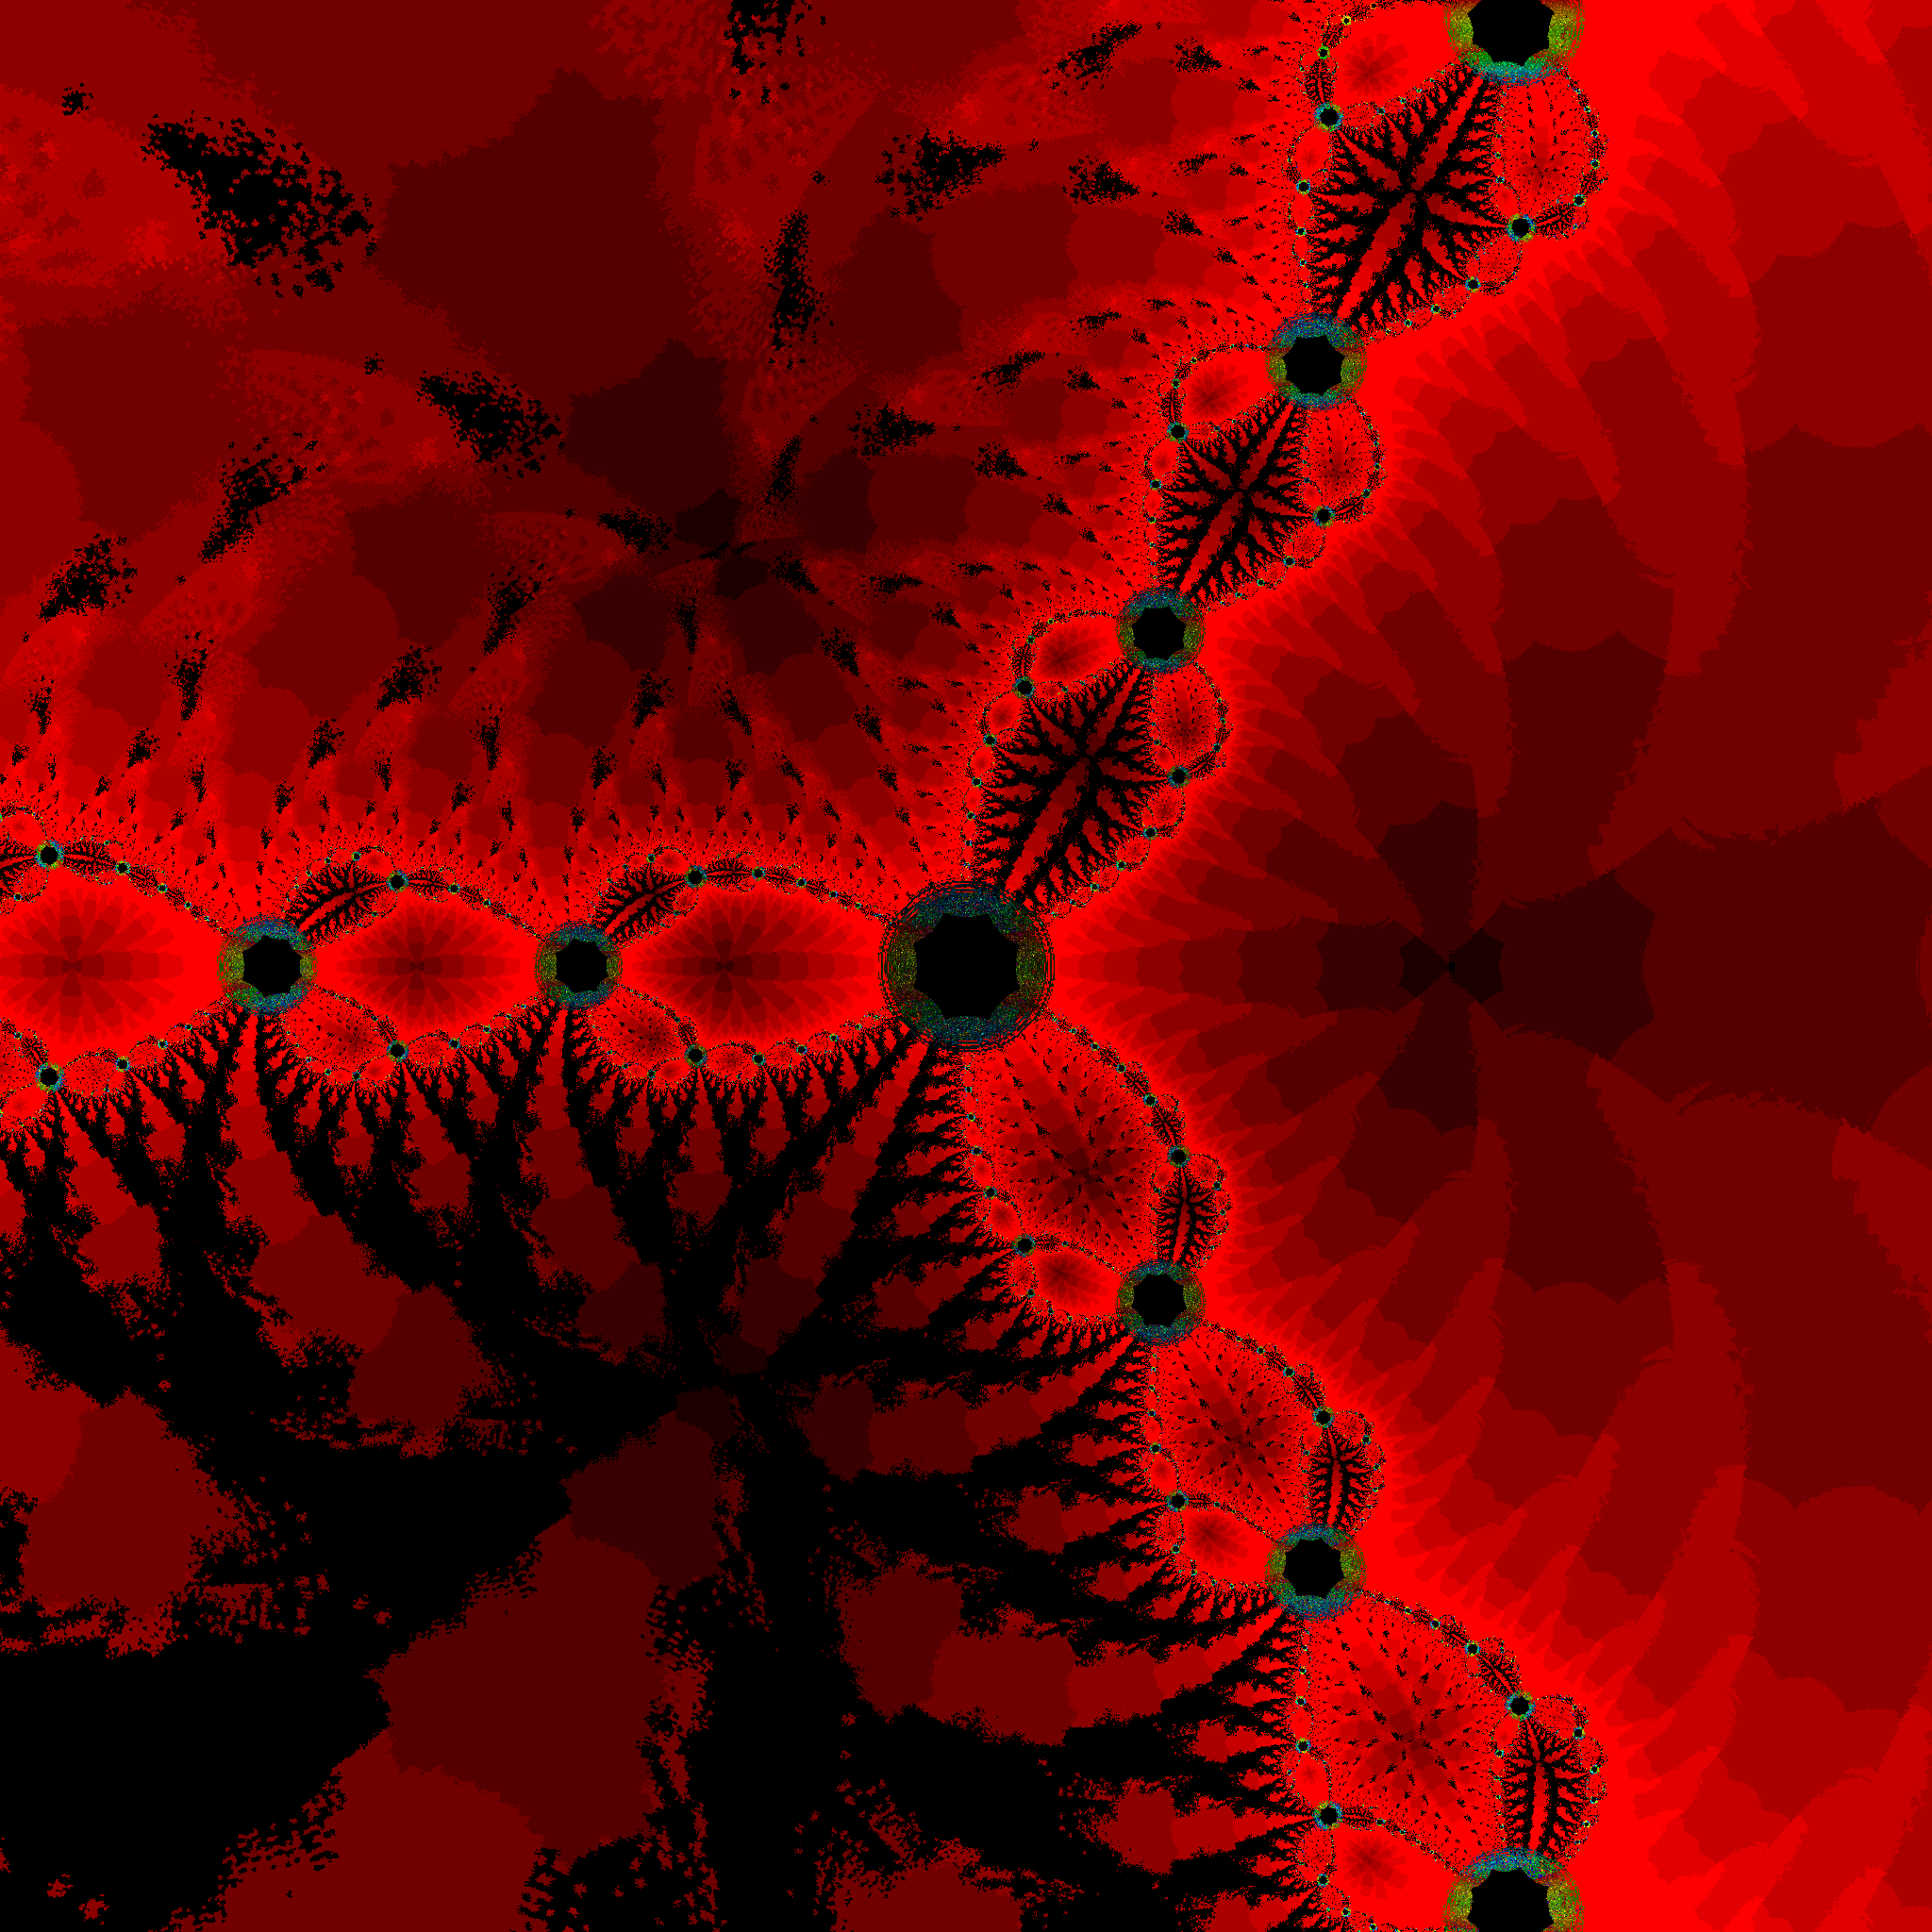
\includegraphics[width=0.35\linewidth]{images/fixed_newton/I22F10_newton.png}
    \end{subfigure}
    \quad
    \caption{Fixed point distortion of Newton's fractal}
    \label{fig:fixed-newton}
\end{figure*}

Figure \ref{fig:1-mantissa} shows this in the Newton fractal. The area close to the origin
maintains high resolution, but it becomes steadily more pixelated
further out. In some sense, this error mirrors the human eye's capabilities:
a foveal region in the center of vision/complex plane.

\setcounter{subsubsection}{798828124}
\subsubsection{Exponent error}

This is the key characteristic of MaskedFloat when configured for
high precision (many mantissa bits)
but a small dynamic range.
The places where the exponent saturates, we introduce distortion. This distortion
appears as arcs of discontinuity in the render. See Figure \ref{fig:3-curves} for a comparison of the f64
rendering of a zoom in of the Mandelbrot fractal and
MaskedFloat (configured with 4 exponent bits and 51 mantissa bits.) 

\setcounter{subsection}{74}
\subsection{A note on dynamic range}
\label{hdr}

For the fractals of interest, coloring a point involves iterating on a value.
Since in many of the numerical formats, larger numbers means large possible errors,
the range of values this calculation reaches matters.

This affects how much distortion we see in the Mandelbrot fractal compared to 
Newton: in the Mandelbrot set, the iterated values tend to stay near their starting
point, or become larger than our escape threshold 4, but in the Newton
fractal, intermediate values can become very large when the slope is near zero,
and the final numbers are very small, as $f(z)$ approaches zero. 

\setcounter{section}{3}
\section{Which pictures are prettiest?}

You may also be interested in one of the threads near the source code \cite{github:thread},
where we have noted regions of interest.

\setcounter{subsection}{142578124}
\subsection{If it's fixed, it's broken}

Figures \ref{fig:1-nozoom} and \ref{fig:1-zoom} don't do a lot to recommend fixed-point to us.
Pixelation can be nice if you're a child of the 80s or something, but it's not really weird enough
that we should use a whole new numeric format. Just use ImageMagick. \cite{imagemagick} \cite{imagemagick:xkcd}

The Newton fractal is a different story, as already shown in Figure \ref{fig:1-mantissa}. Since the Newton fractal may result in very small or very
large intermediate values, fixed-point numbers are uniquely poorly suited
for accurate computation. In Figure \ref{fig:fixed-newton},
we can see a nice fractal visualization of approaches to zeros become a fractal hellscape of 
non-convergence and incorrect answers, by switching from \texttt{f64} to \texttt{I22F10}. 
Despite no longer containing useful information, the distorted Newton's fractal looks much cooler.

%% /mandelbrot/?x=15533894506455&y=5083731656658&window=67108864&scale=42364430472150&res=2048&iters=300
\begin{figure*}
    \begin{subfigure}[f32]
        \centering
        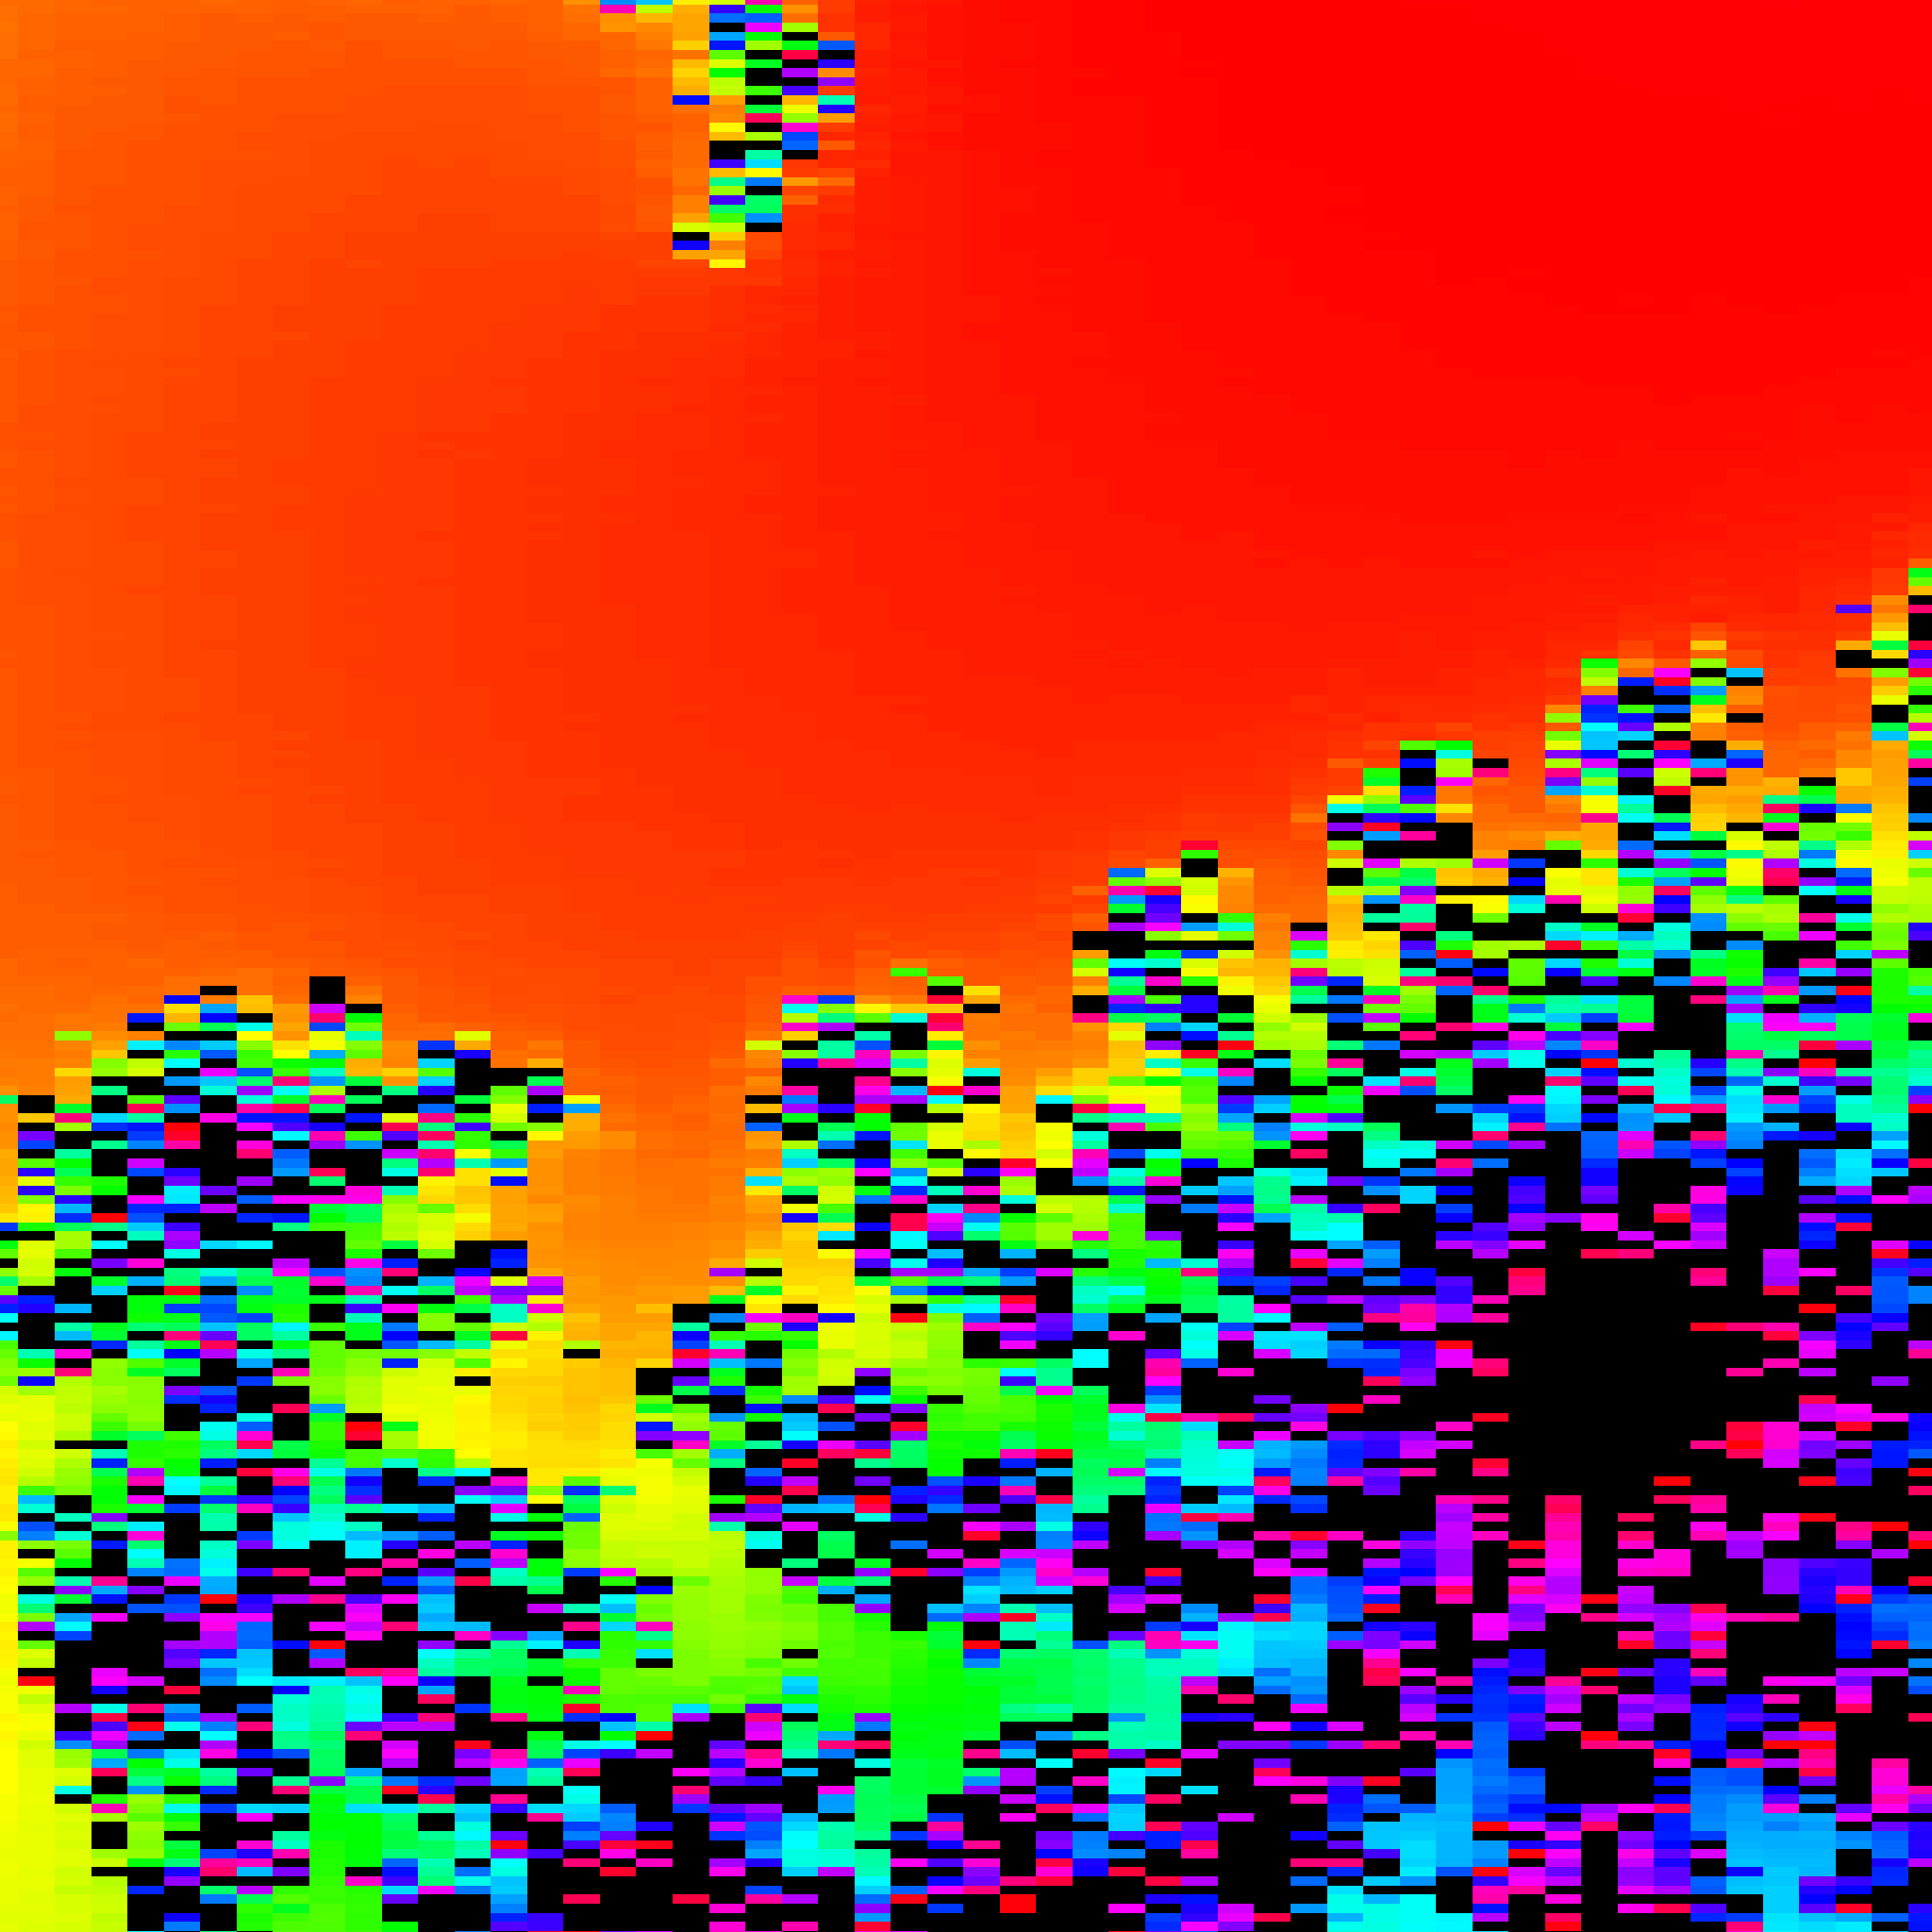
\includegraphics[width=0.31\linewidth]{images/2-posit-pixels/f32.png}
    \end{subfigure}
    \quad
    \begin{subfigure}[f64]
        \centering
        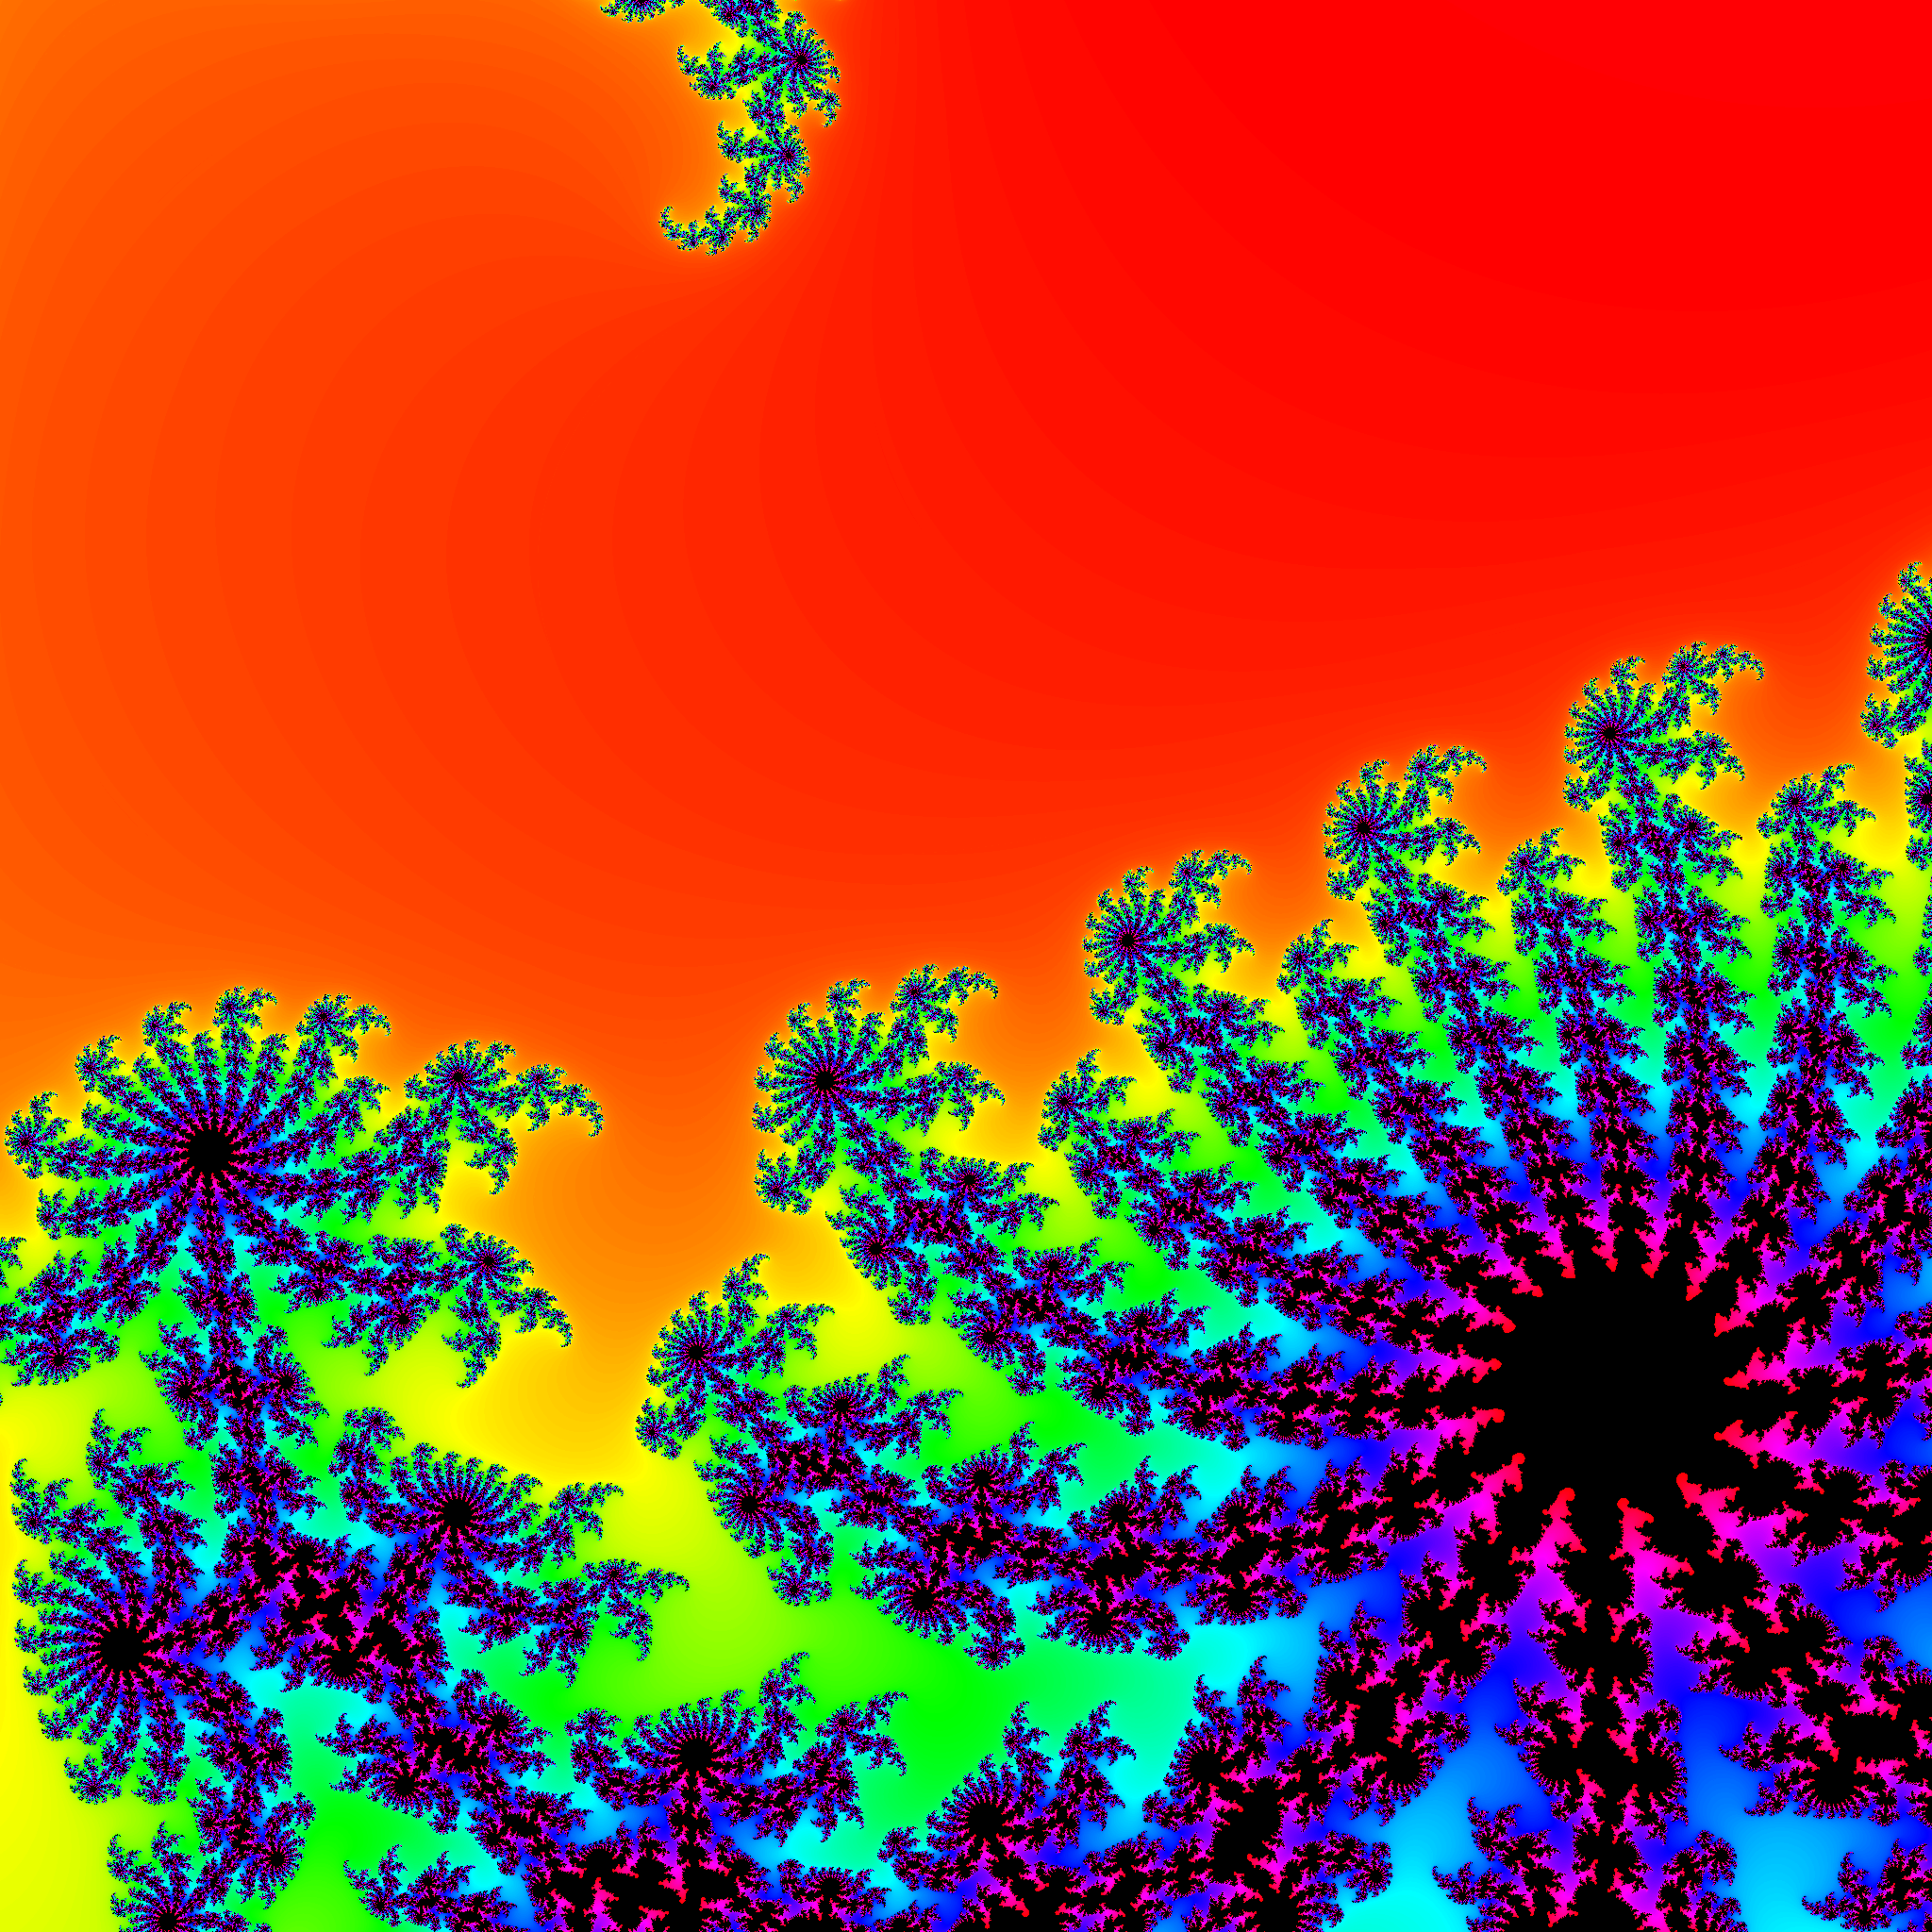
\includegraphics[width=0.31\linewidth]{images/2-posit-pixels/f64.png}
    \end{subfigure}
    \quad
    \begin{subfigure}[P32]
        \centering
        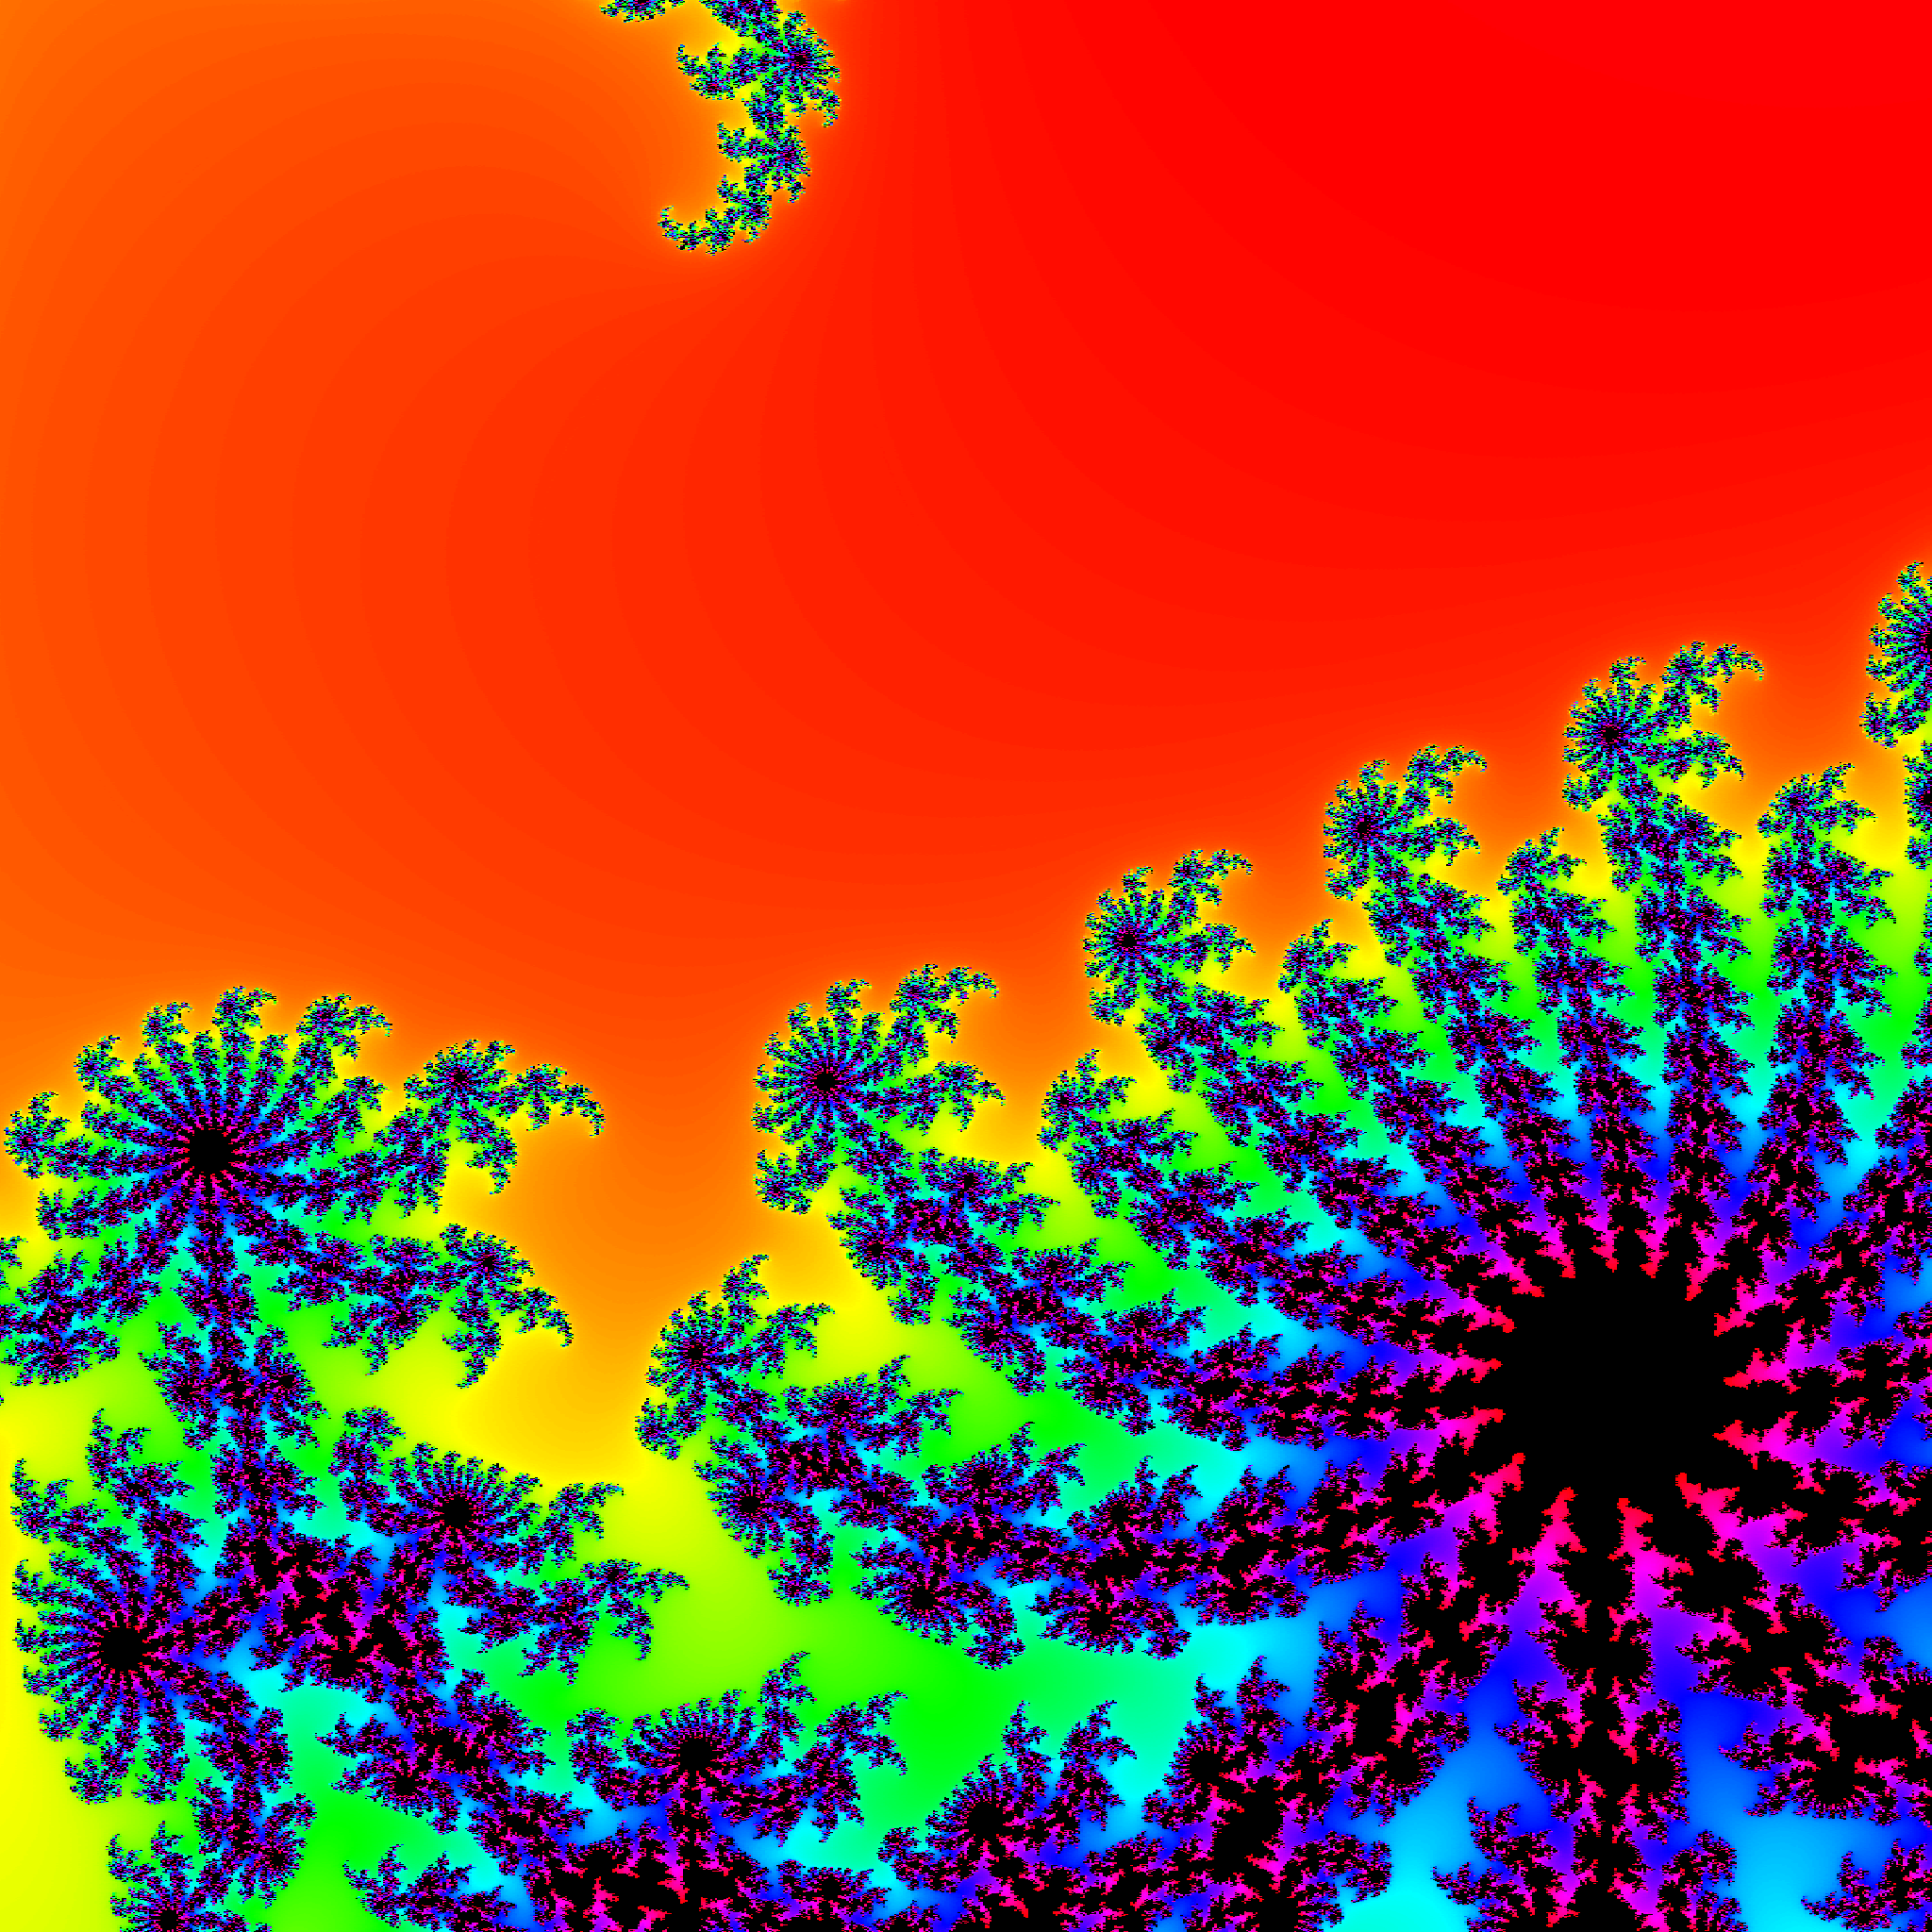
\includegraphics[width=0.31\linewidth]{images/2-posit-pixels/P32.png}
    \end{subfigure}
    \caption{f32, f64, and P32 over a whorl}
    \label{fig:2-posit-pixels}
\end{figure*}

% /newton/?x=68526&y=-115911&window=32768&scale=93312&res=2048&iters=32
\begin{figure*}
    \begin{subfigure}[P32]
        \centering
        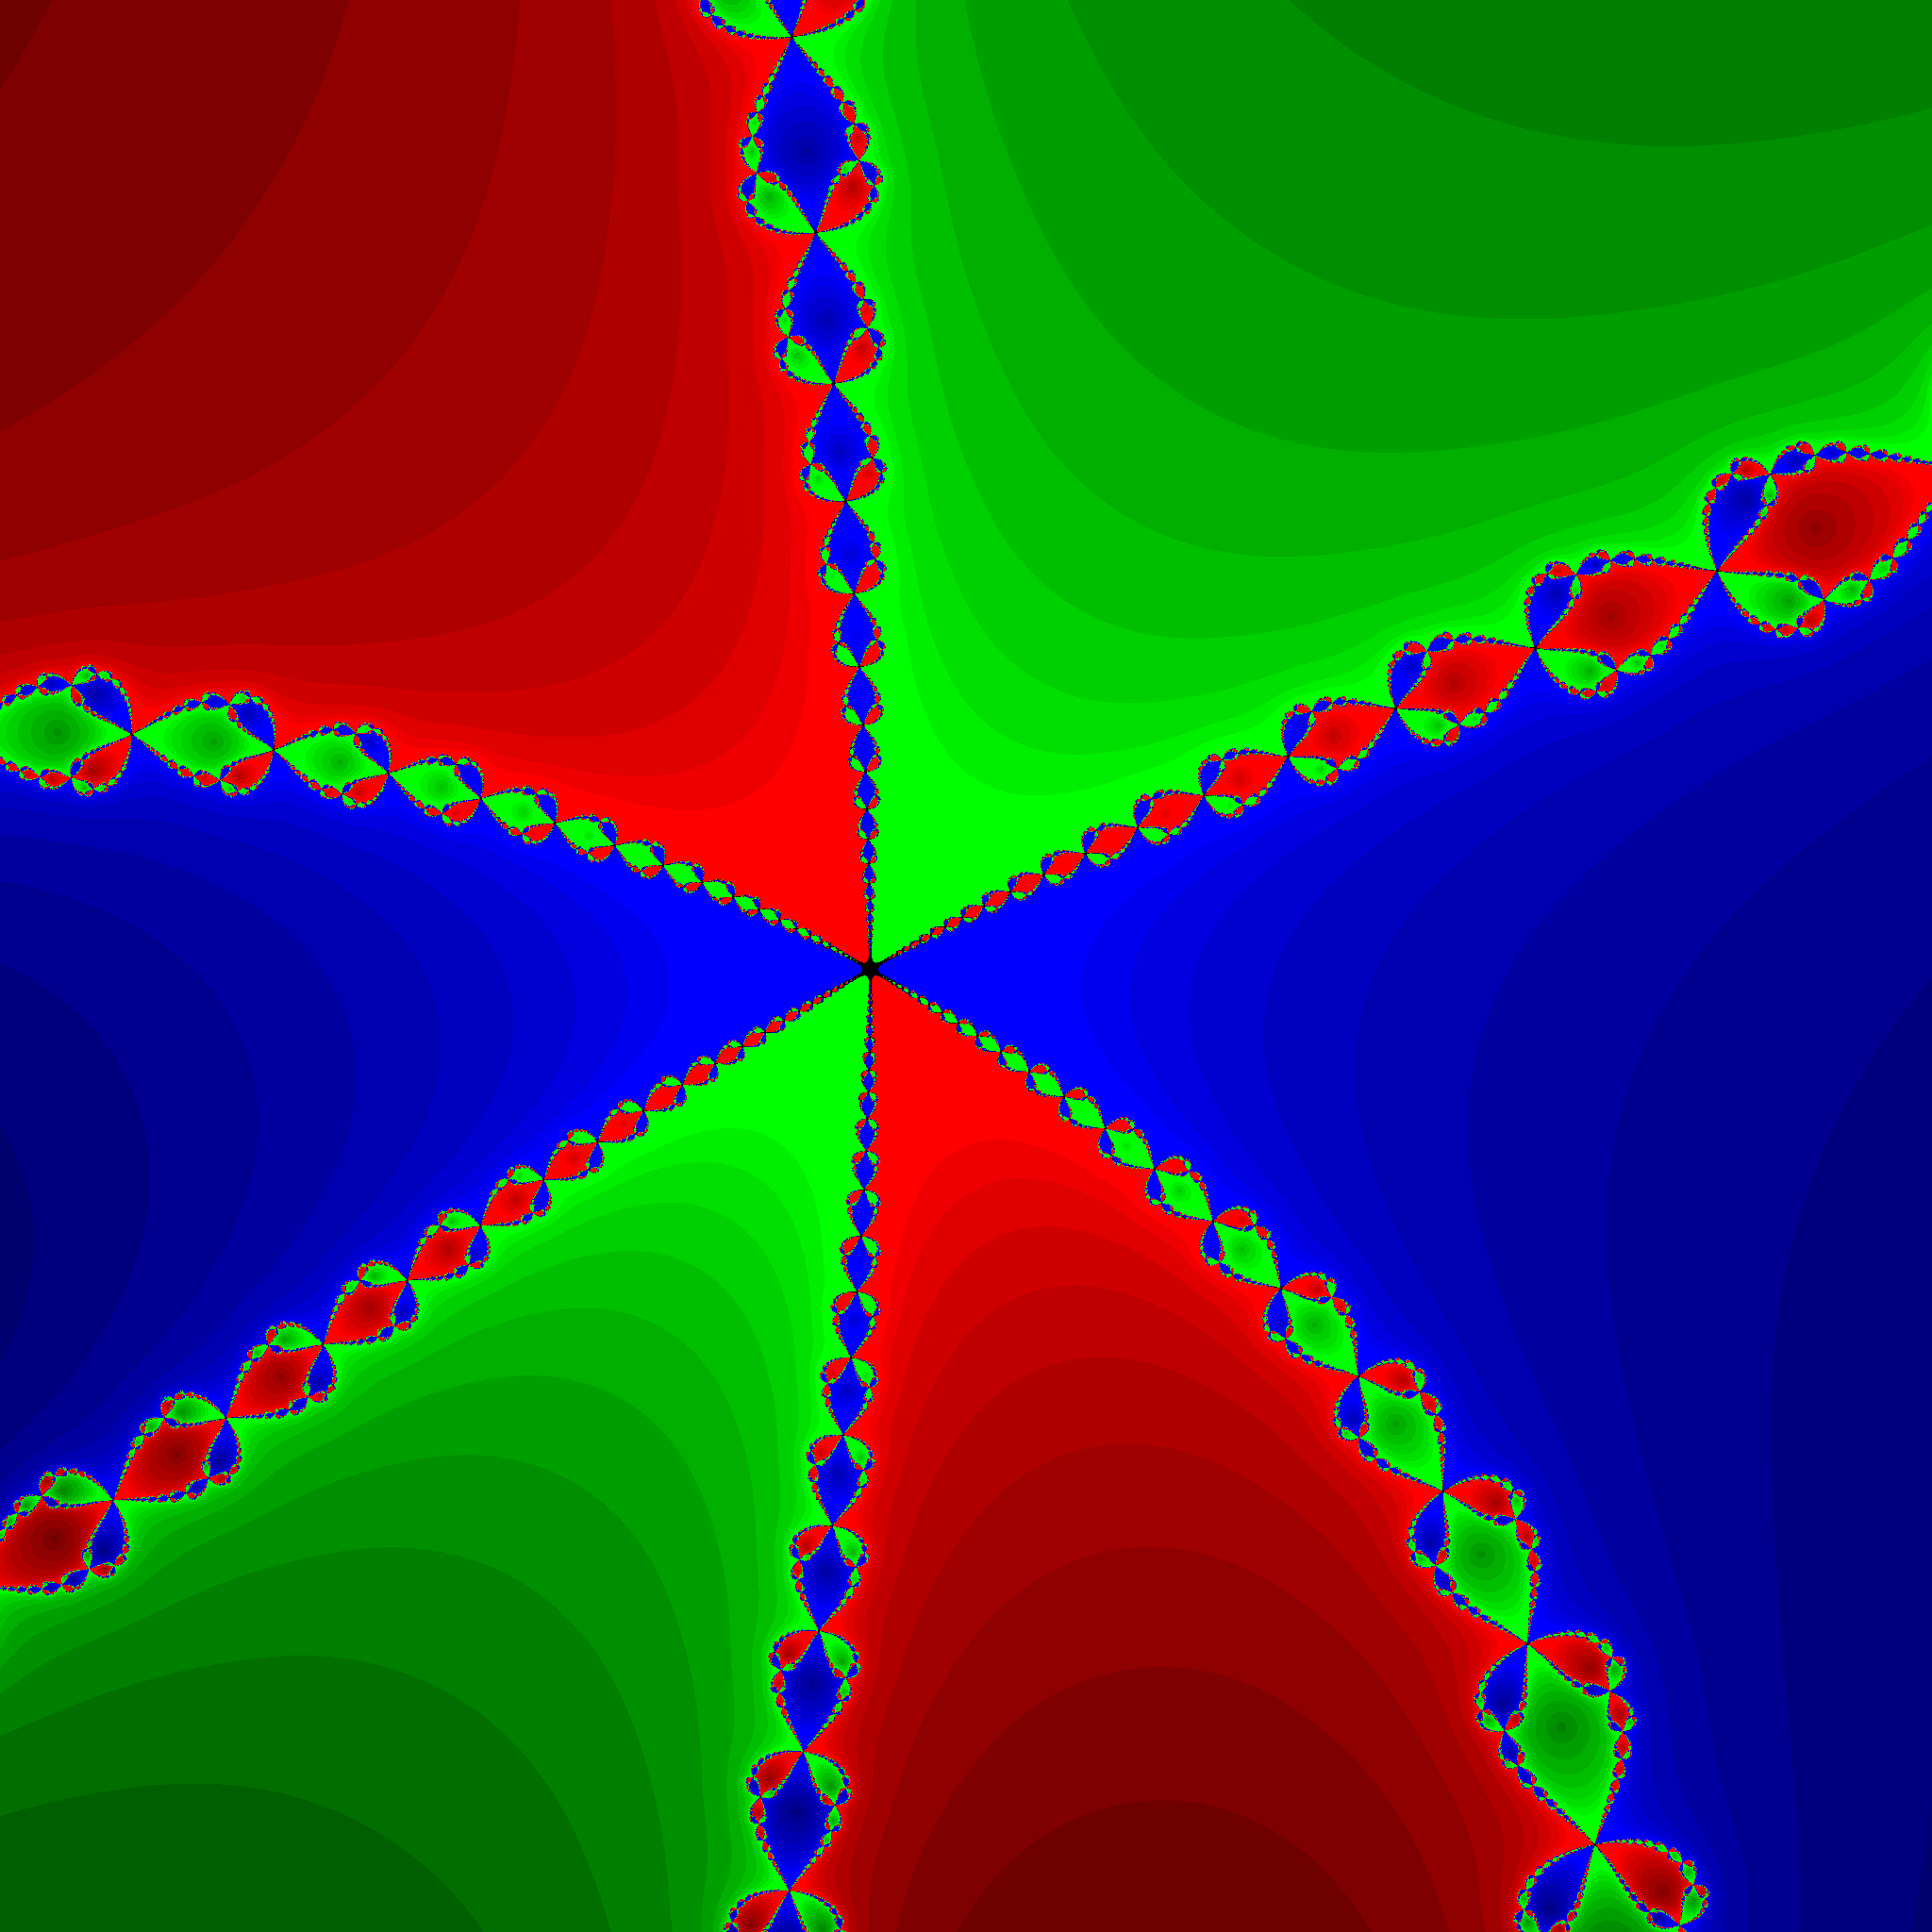
\includegraphics[width=0.31\linewidth]{images/3-newton-ripples/P32.png}
    \end{subfigure}
    \quad
    \begin{subfigure}[P16]
        \centering
        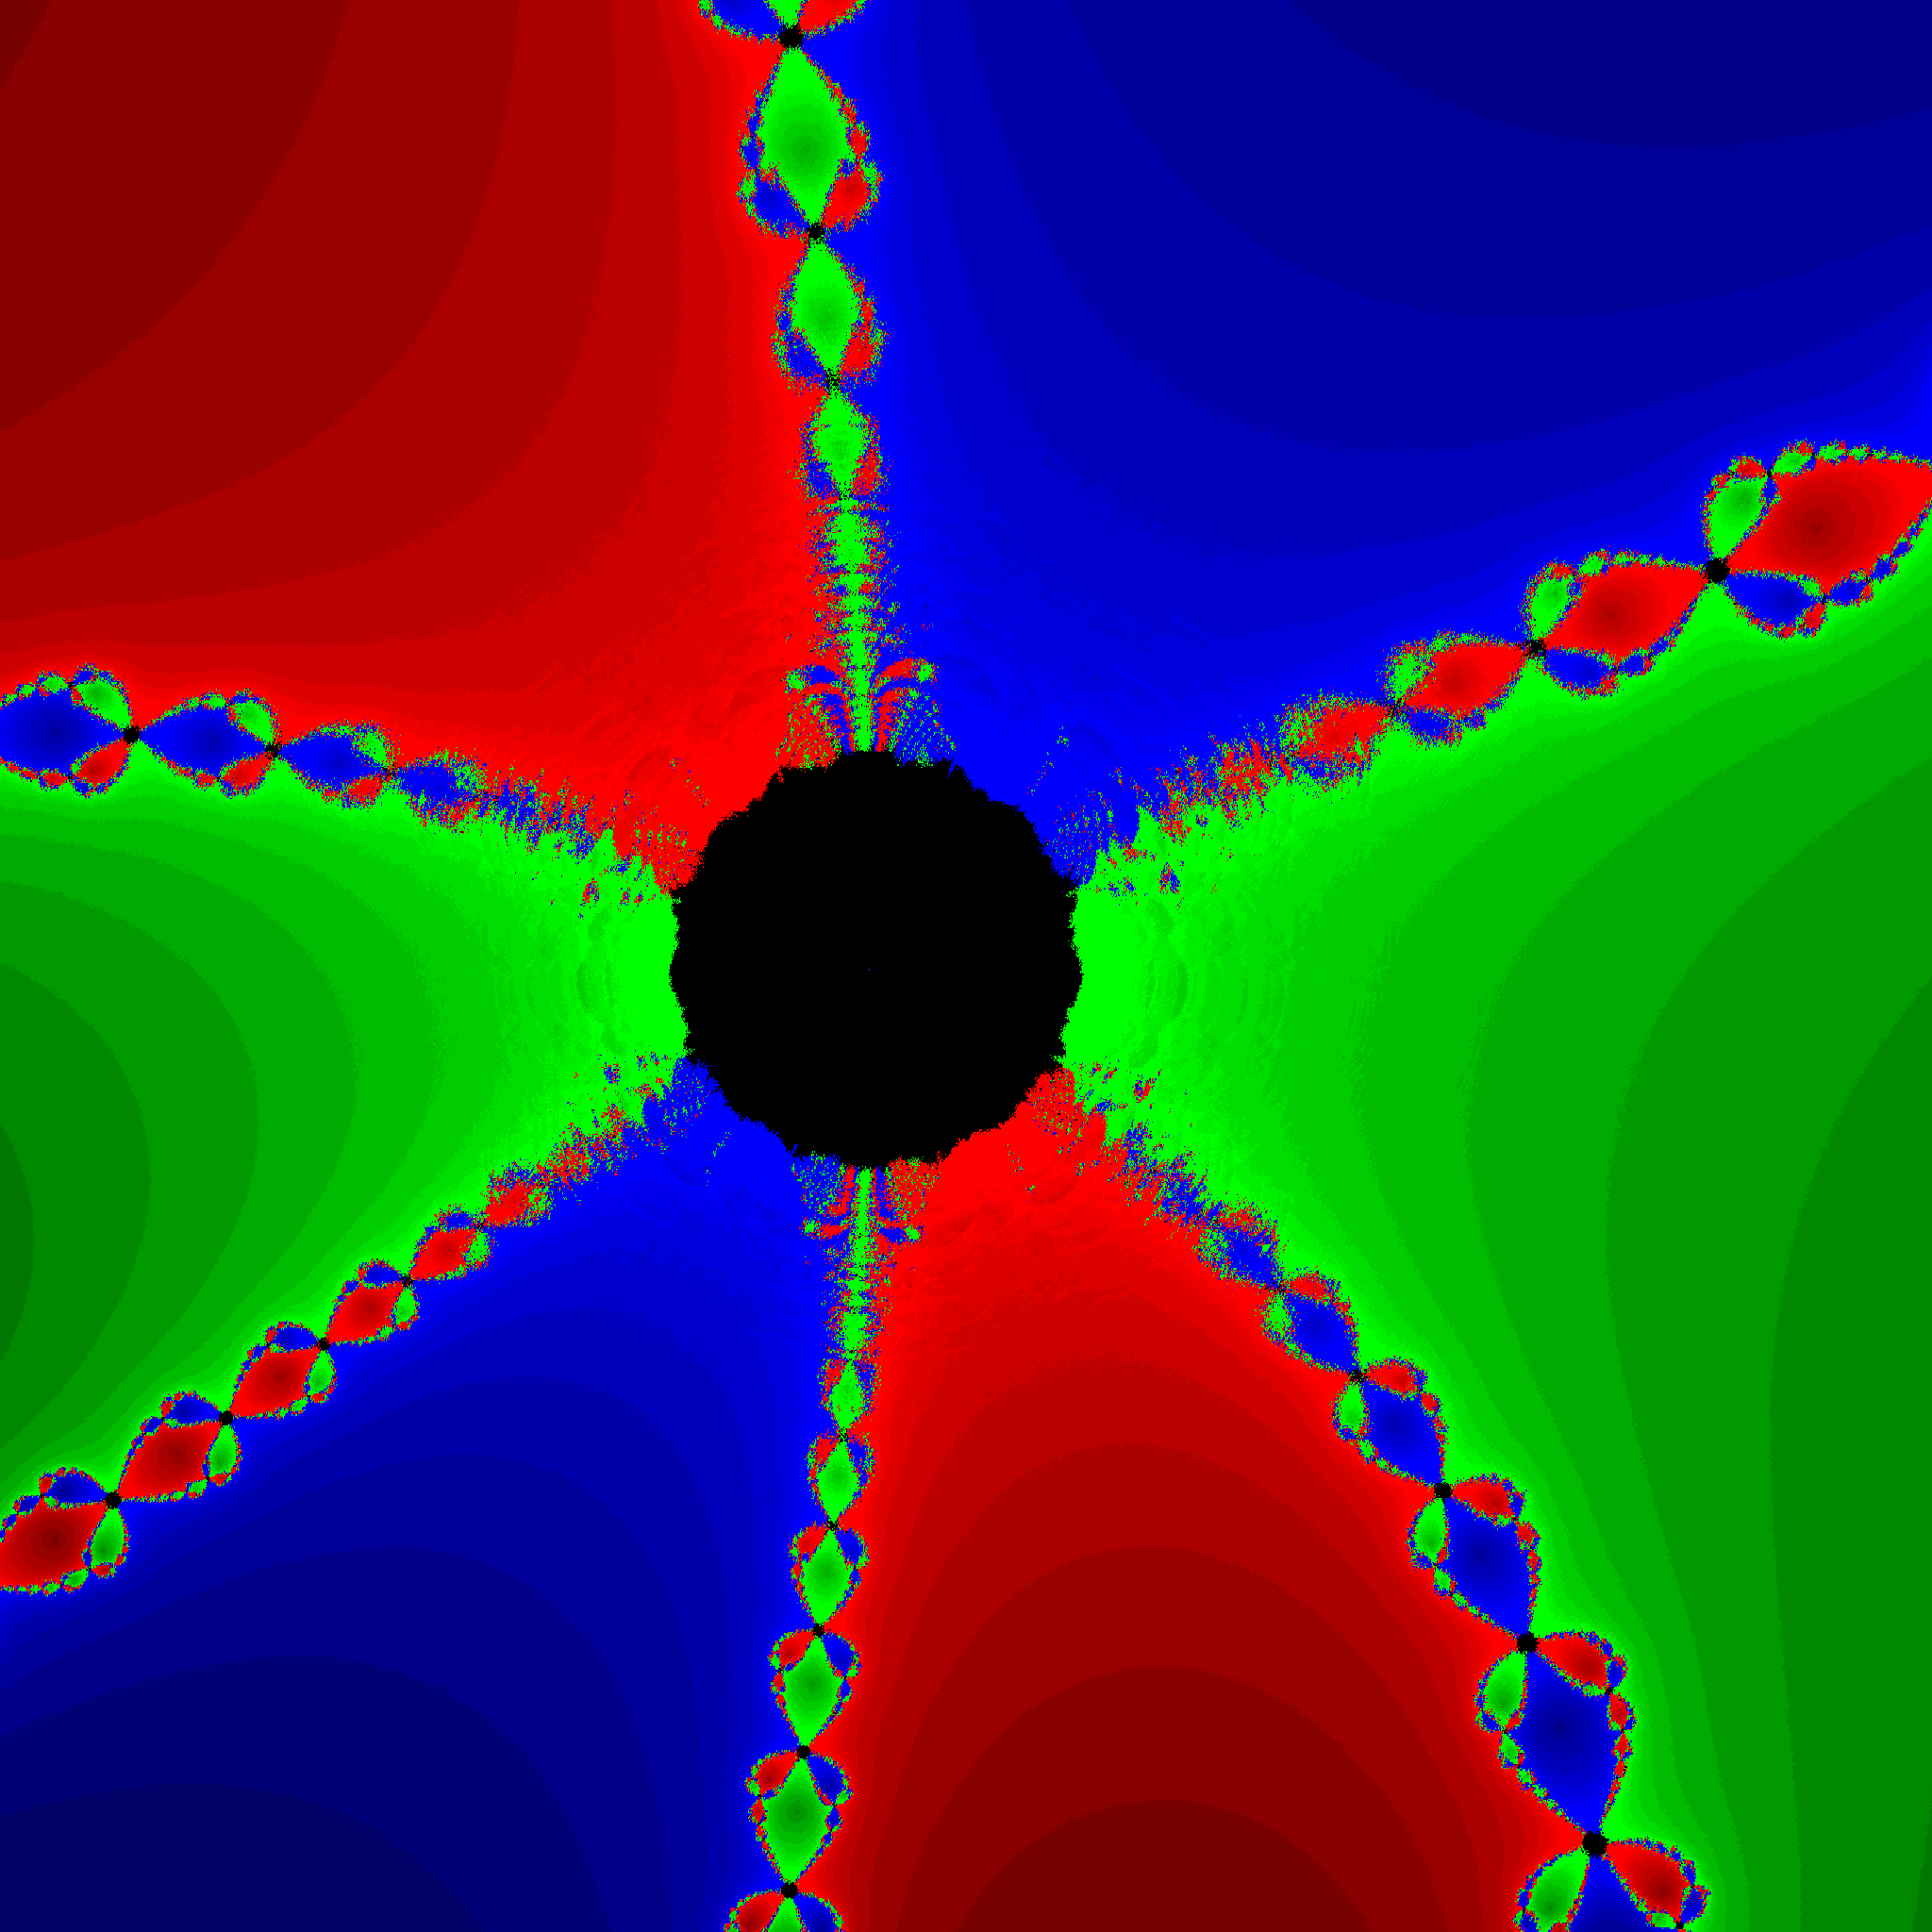
\includegraphics[width=0.31\linewidth]{images/3-newton-ripples/P16.png}
    \end{subfigure}
    \quad
    \begin{subfigure}[MaskedFloat<4,50>]
        \centering
        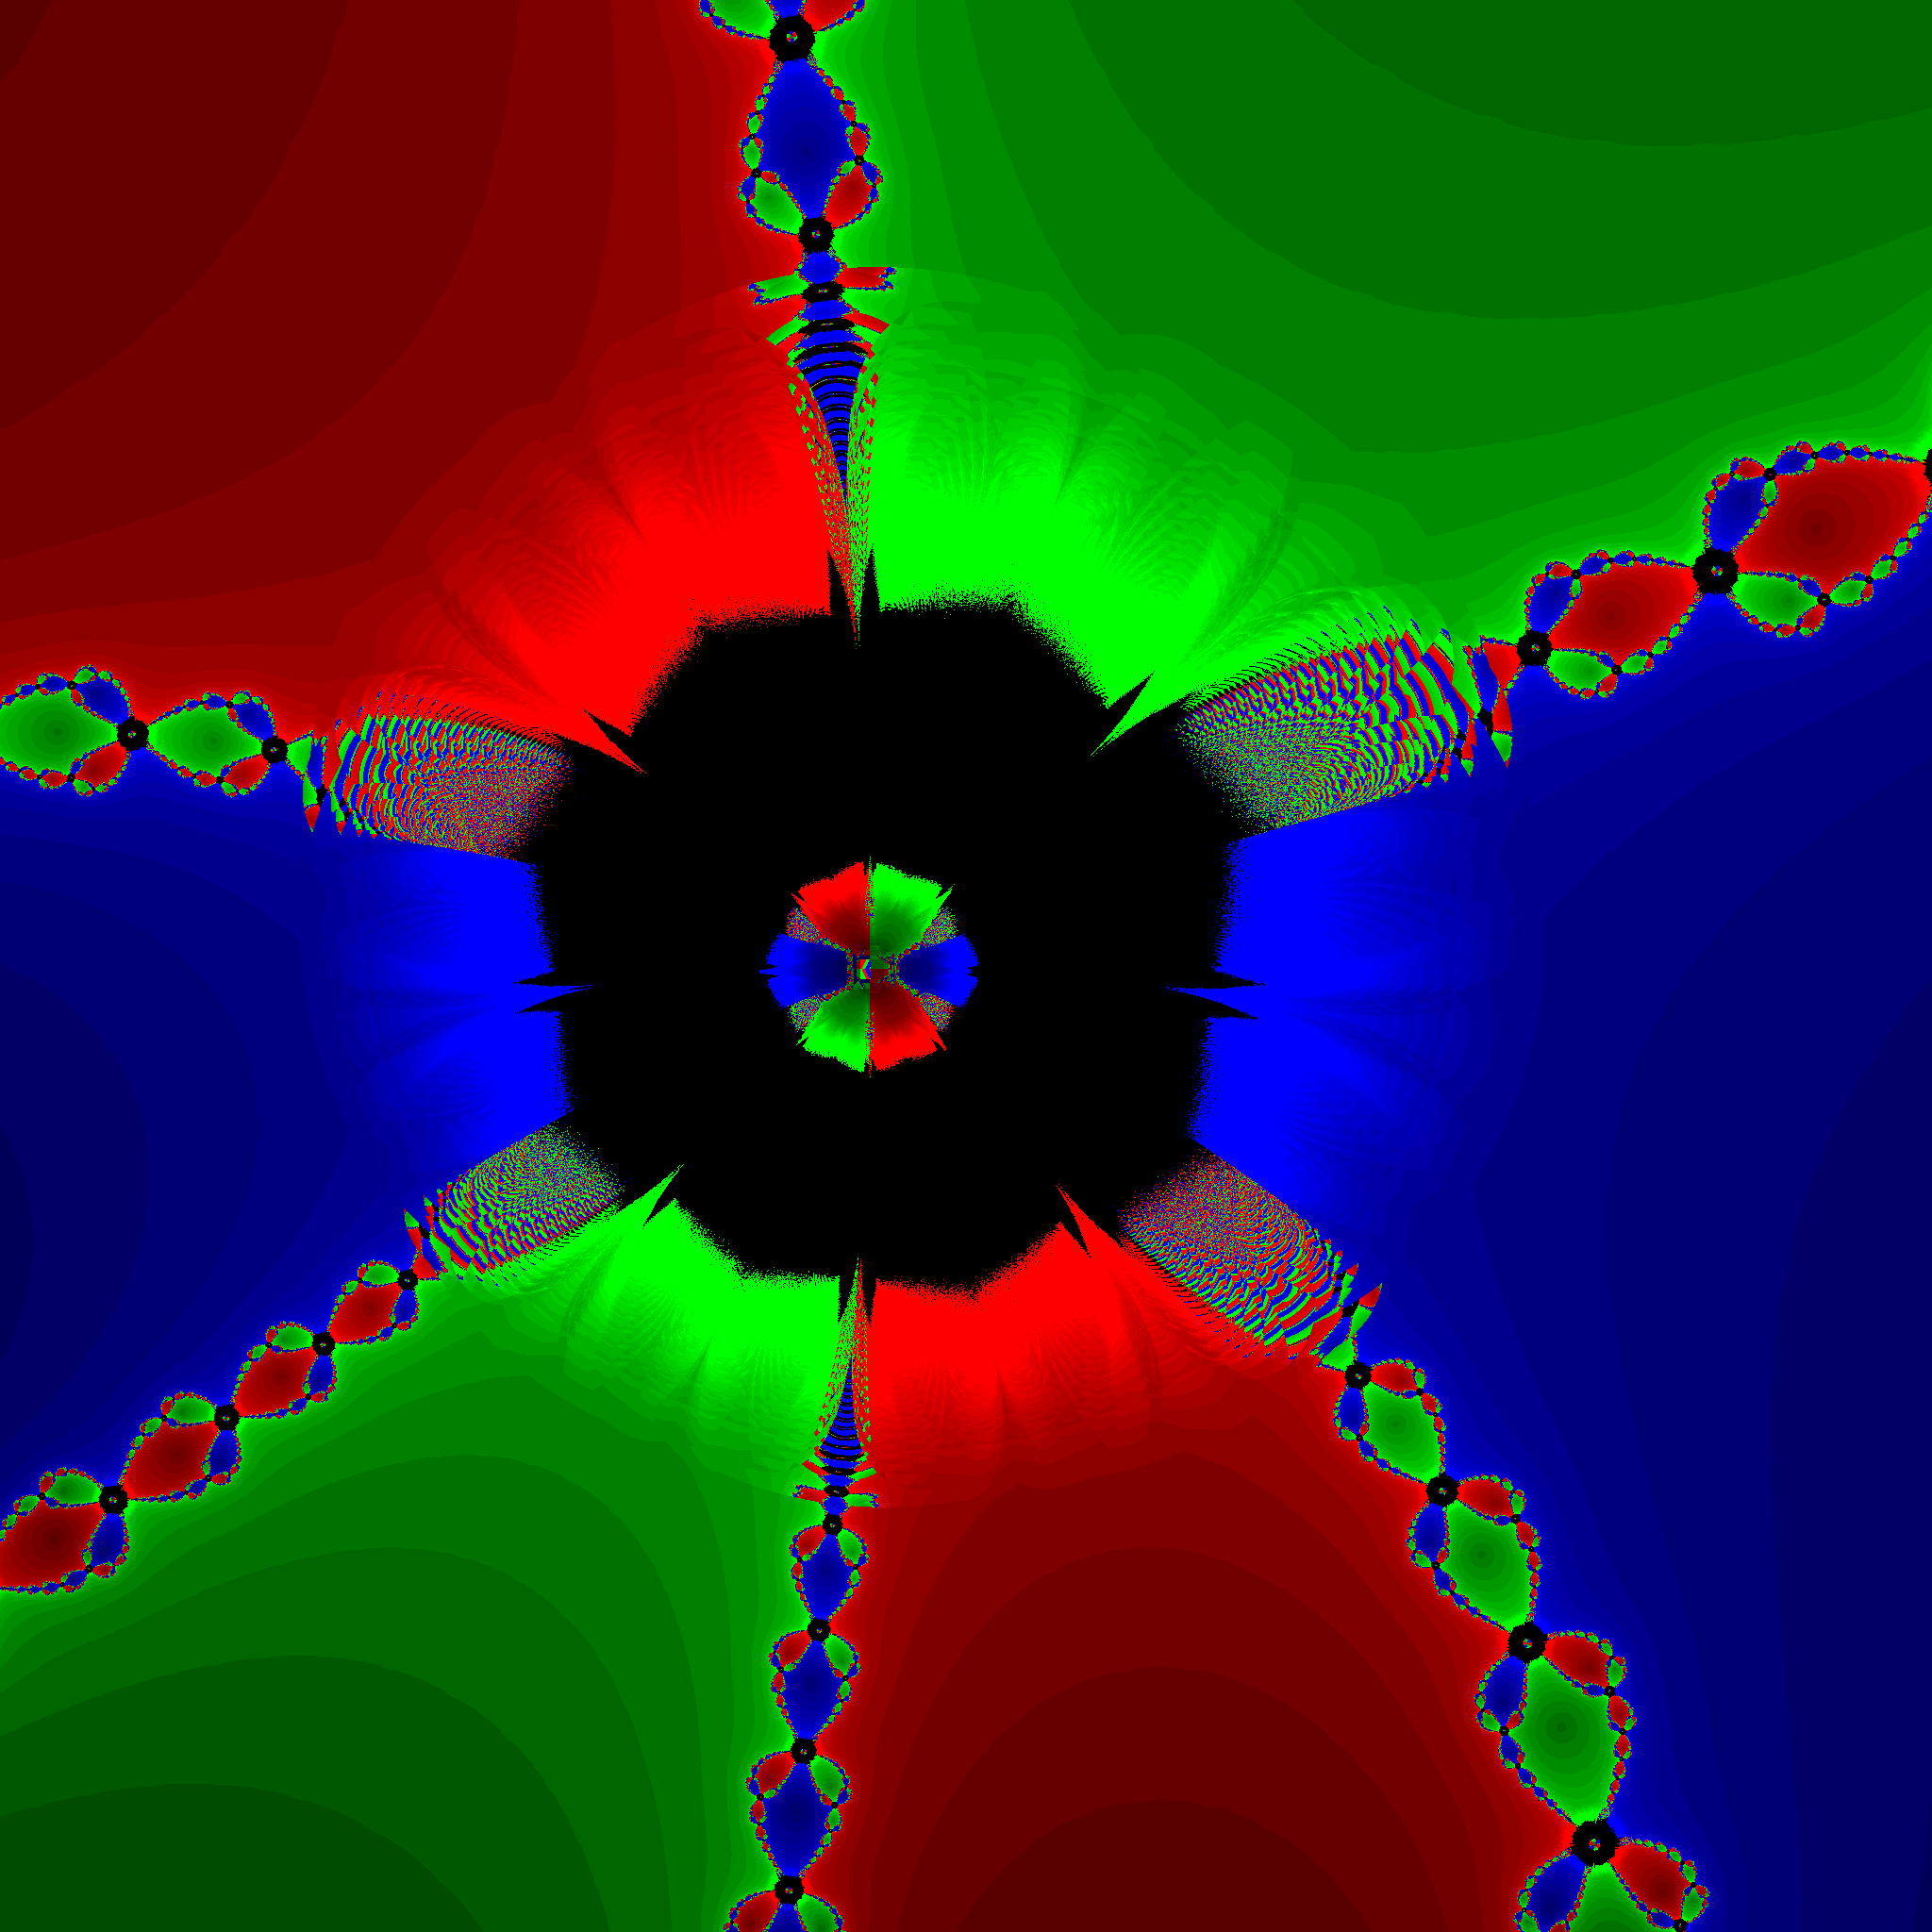
\includegraphics[width=0.31\linewidth]{images/3-newton-ripples/mf4.png}
    \end{subfigure}
    \caption{P32, P16, and MaskedFloat<4,50> on the Newton fractal}
    \label{fig:3-newton-ripples}
\end{figure*}

\FloatBarrier
\setcounter{subsection}{28515624}
\subsection{Pixels and Posits\texttrademark}

Posits\texttrademark  maintain greater precision than \texttt{f32}, with the same number of bits.
Figure \ref{fig:2-posit-pixels} shows \texttt{f32}, \texttt{f64}, \texttt{P32} over the same area.

Clearly posits\texttrademark are the best option for everything. Right? Come. Follow the word of Gustafson. \cite{posit} Enter the circle between zero and infinity. join us Join Us JOIN US 

Sorry, got a little chanty there--didn't mean to scare you. Can we interest you in an informative pamphlet? \cite{cult}

\setcounter{subsection}{427734374}
\subsection{Newtonian surfaces}

Let's face it, there's a reason that Mandelbrot is popular: there's lots of different shapes and colors.
But despite being less popular, Newton fractals have some interesting artifacts too! Seriously! Promise!

Like Figure \ref{fig:3-newton-ripples}: floating-point and \texttt{P32} formats all run up against the iteration limit at the center area. However, evaluation at higher iterations "closes" the hole (not shown).

\texttt{P16}, though, runs up against its limits, rippling out noise and forming a hole in the center, which persists at higher iterations. MaskedFloat goes even further and produces a distorted mirror within the empty space.

It's a little creepy, honestly. Have you seen \ref{sphere}? It's like that. Right? Right.

\setcounter{subsection}{572265624}
\subsection{Newtonian event horizons}

\begin{figure*}
    \begin{subfigure}[F32]
        \centering
        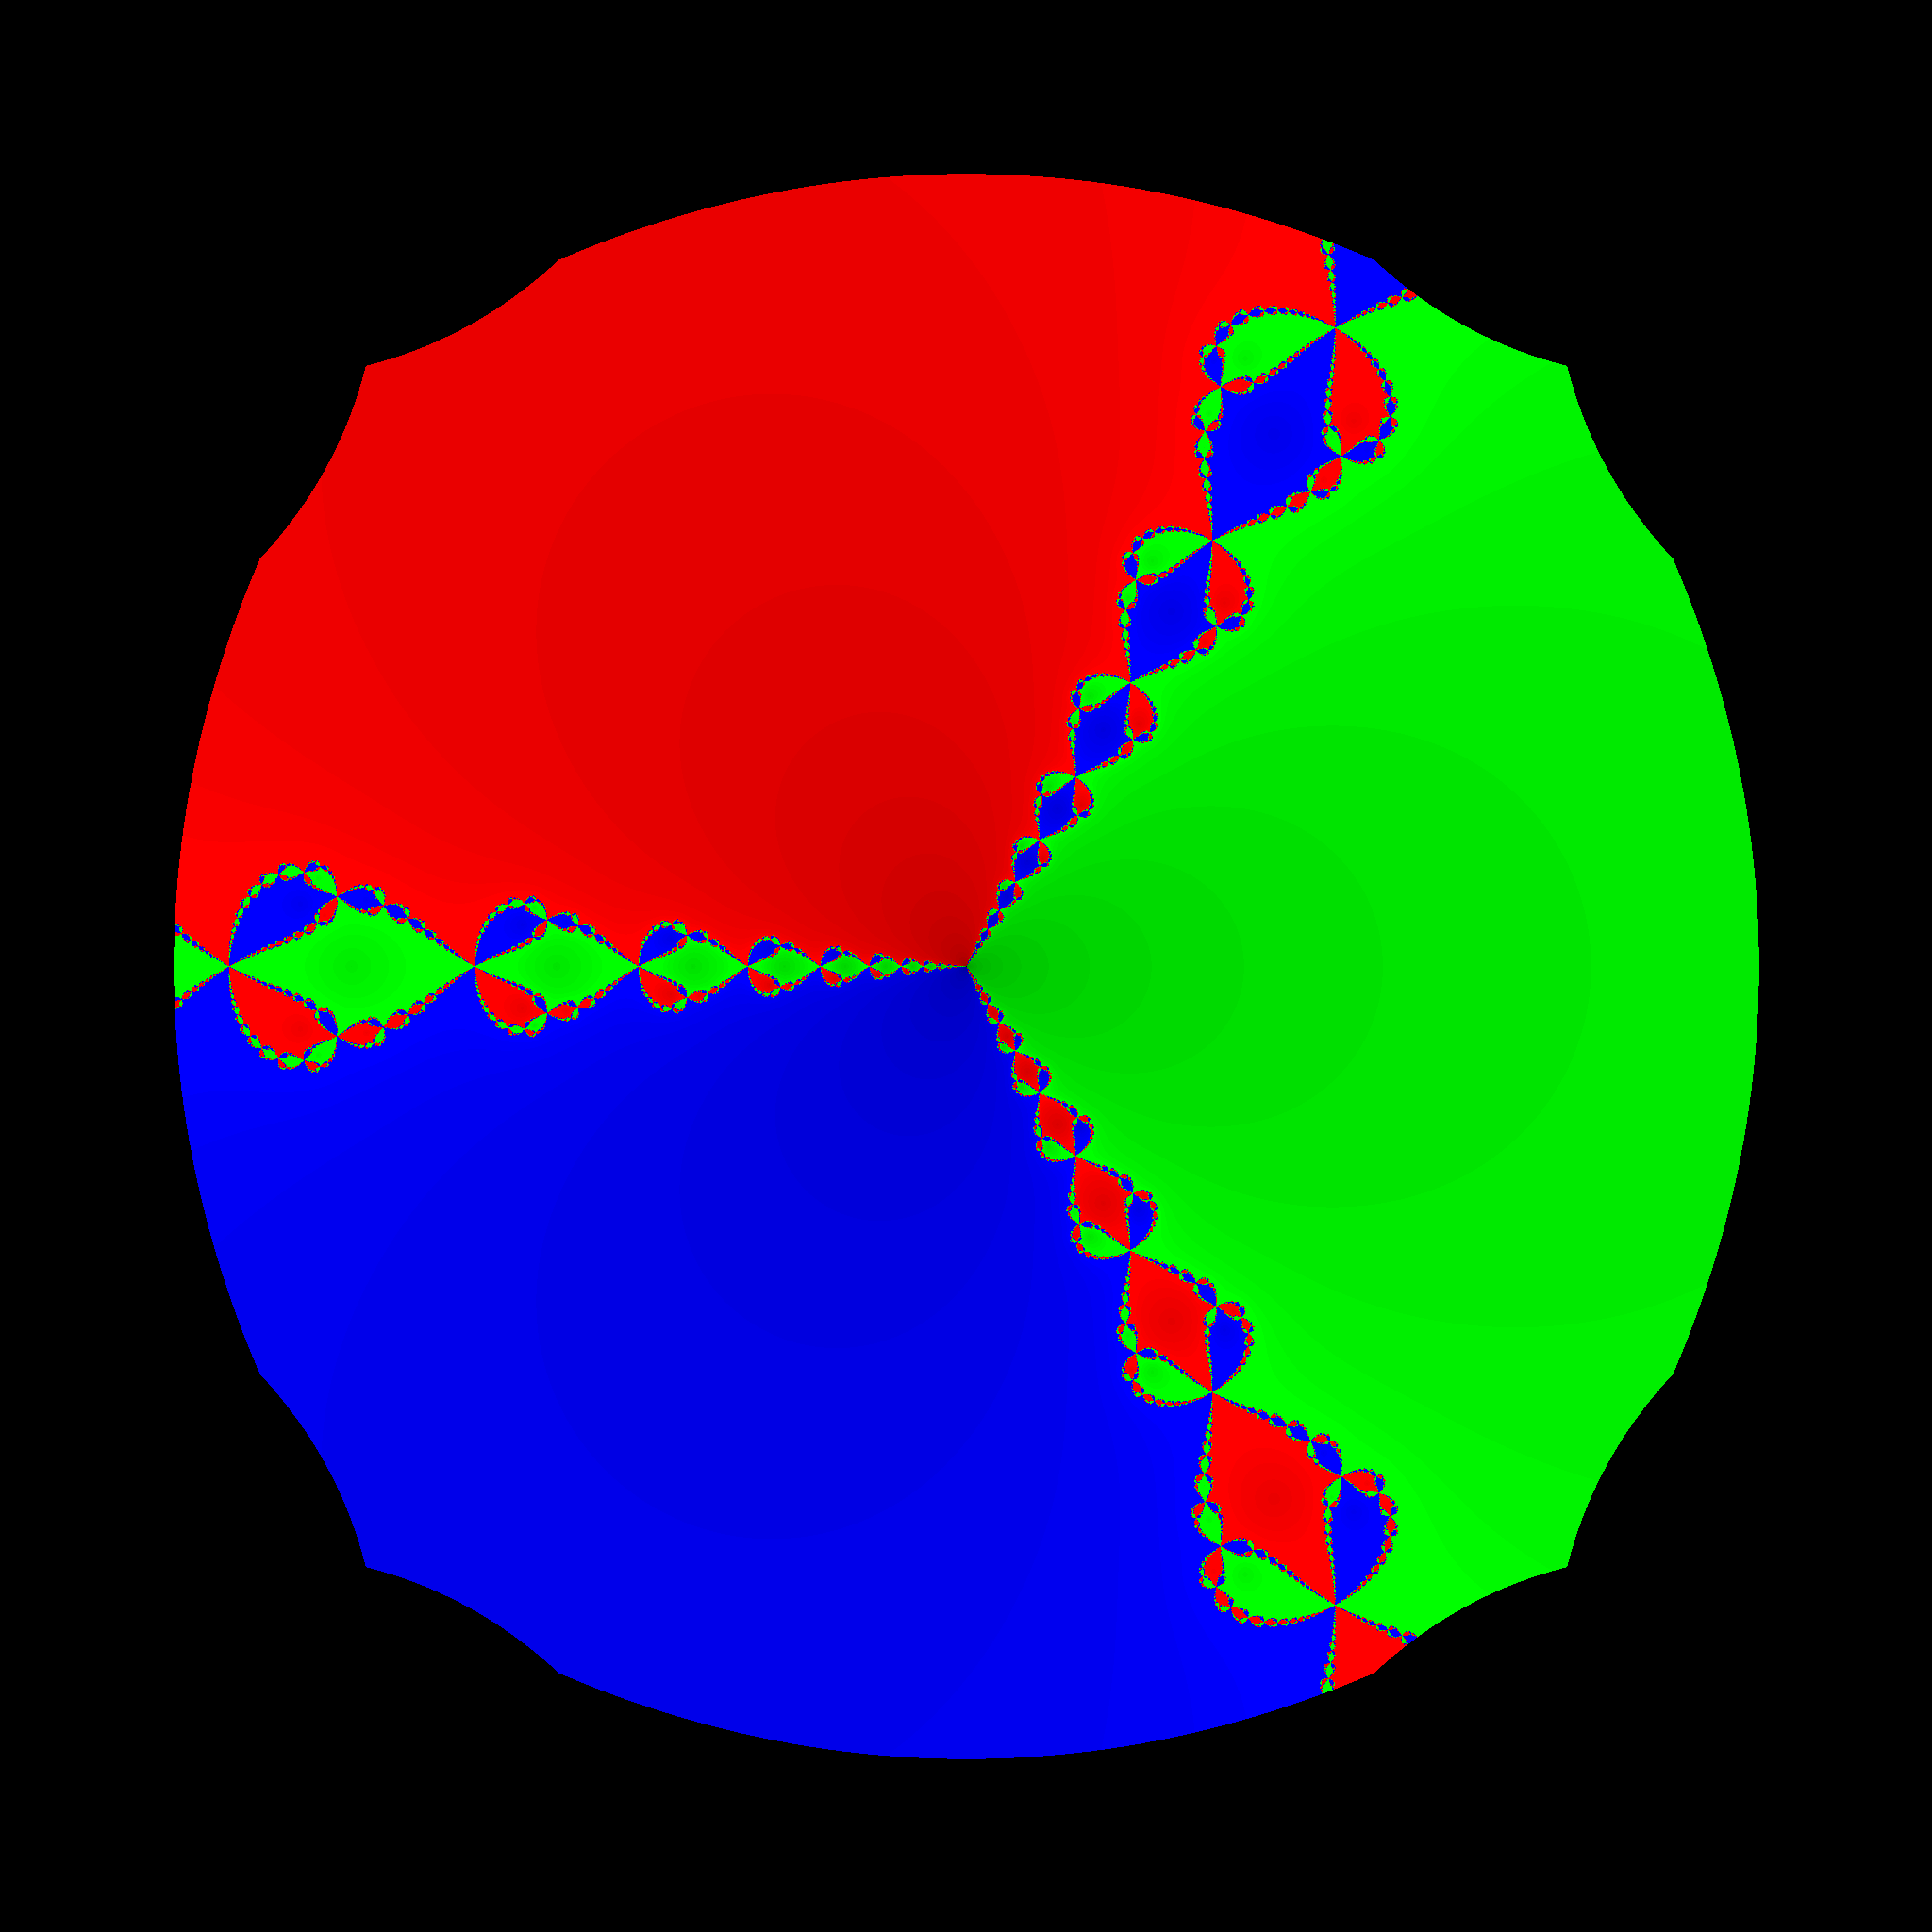
\includegraphics[width=0.23\linewidth]{images/event_horizon/f32_horizon.png}
    \end{subfigure}
    \quad
    \begin{subfigure}[P16]
        \centering
        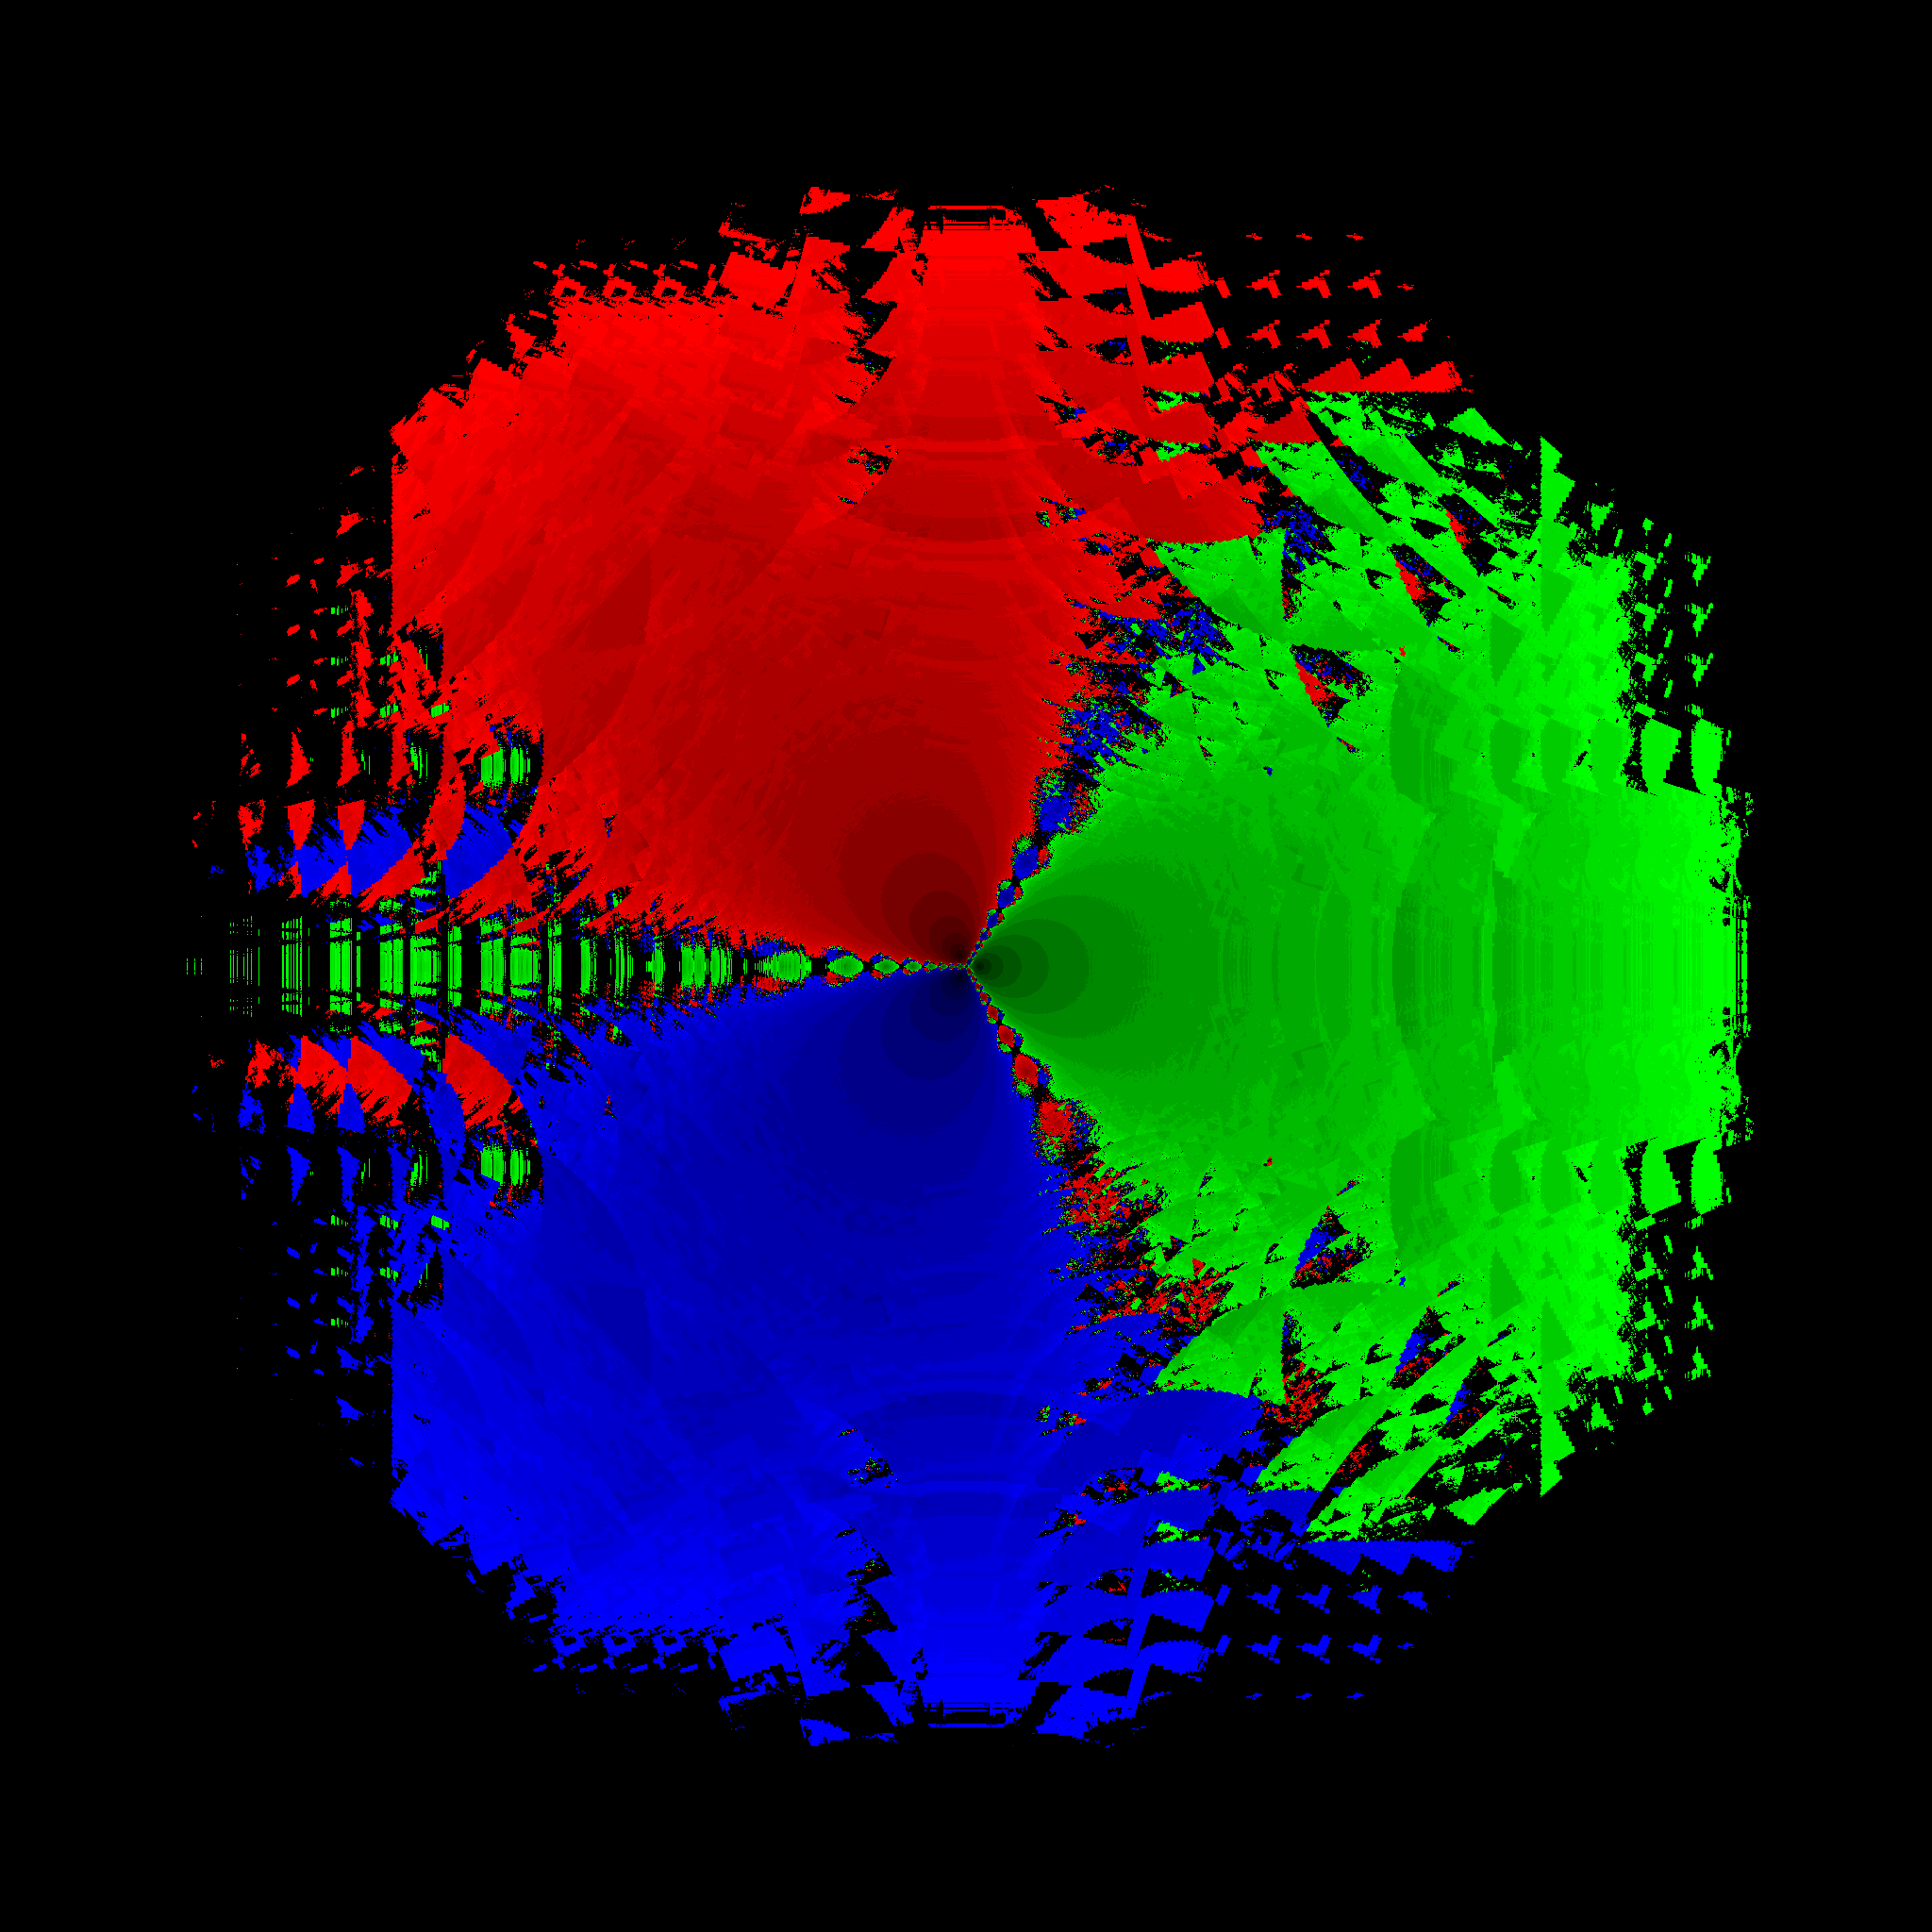
\includegraphics[width=0.23\linewidth]{images/event_horizon/P16_horizon.png}
    \end{subfigure}
    \quad
    \begin{subfigure}[MaskedFloat<4,50>]
        \centering
        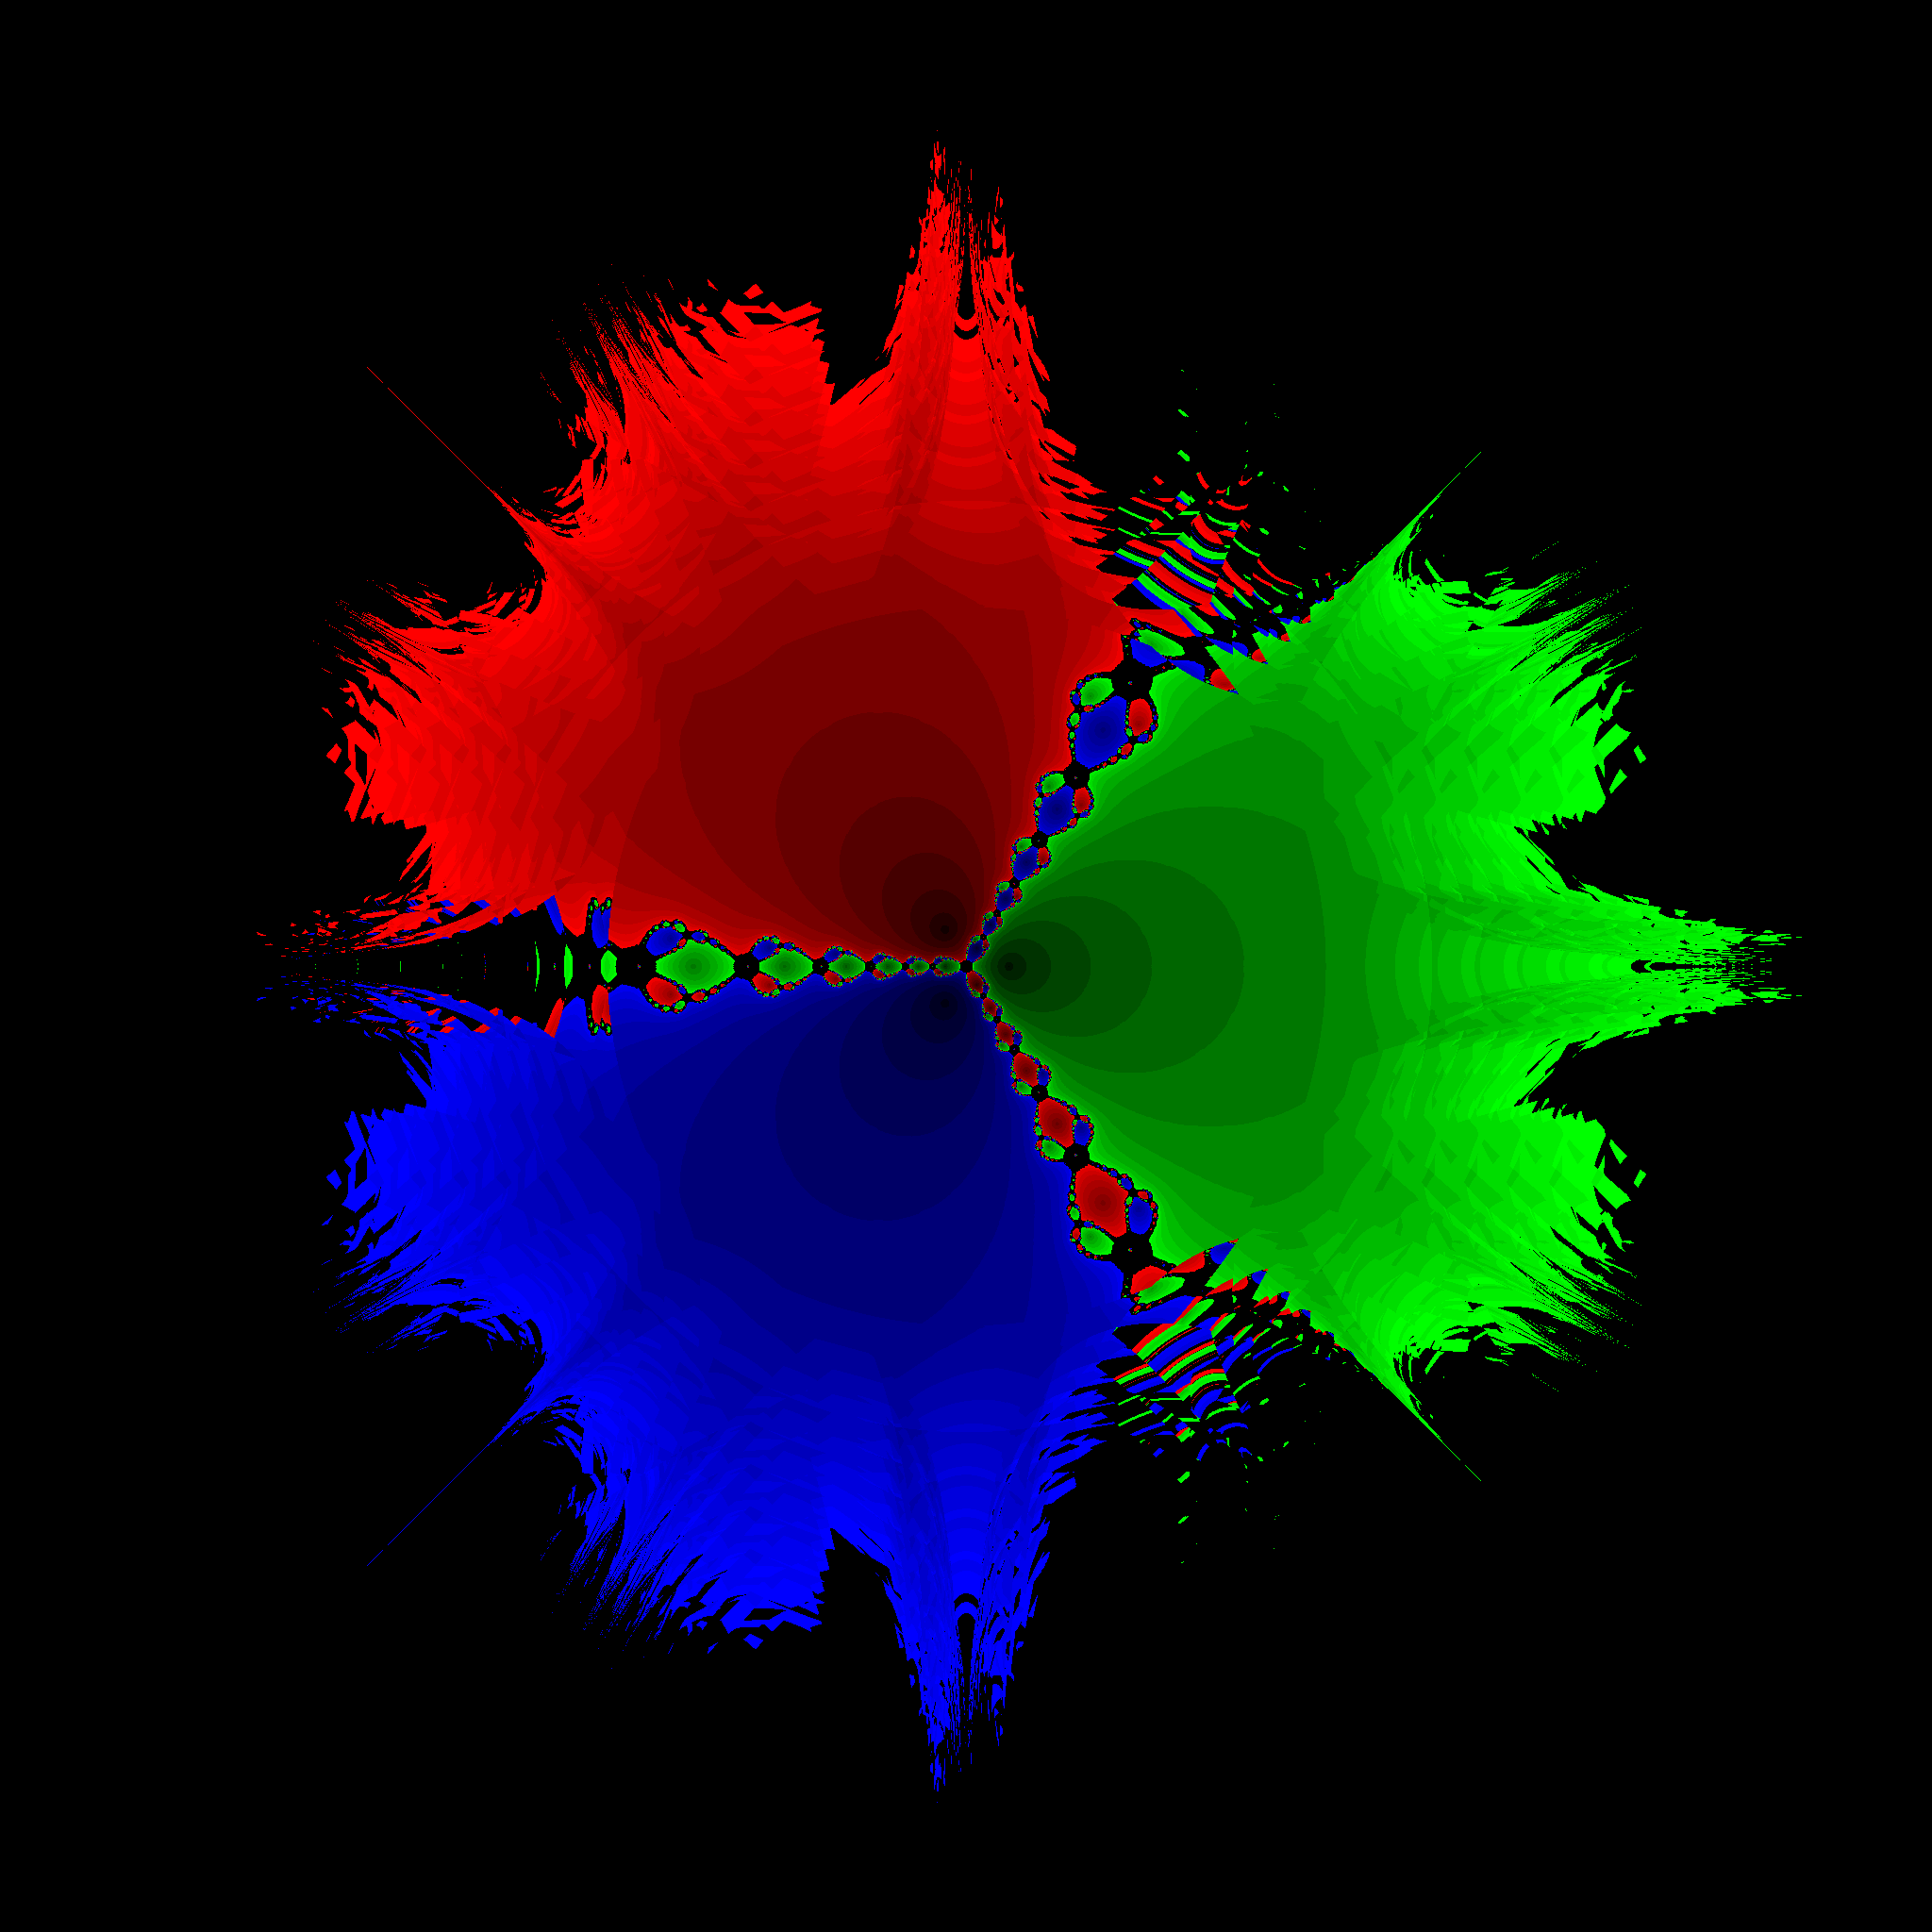
\includegraphics[width=0.23\linewidth]{images/event_horizon/MaskedFloat_4_50_horizon.png}
    \end{subfigure}
    \quad
    \begin{subfigure}[I22F10]
        \centering
        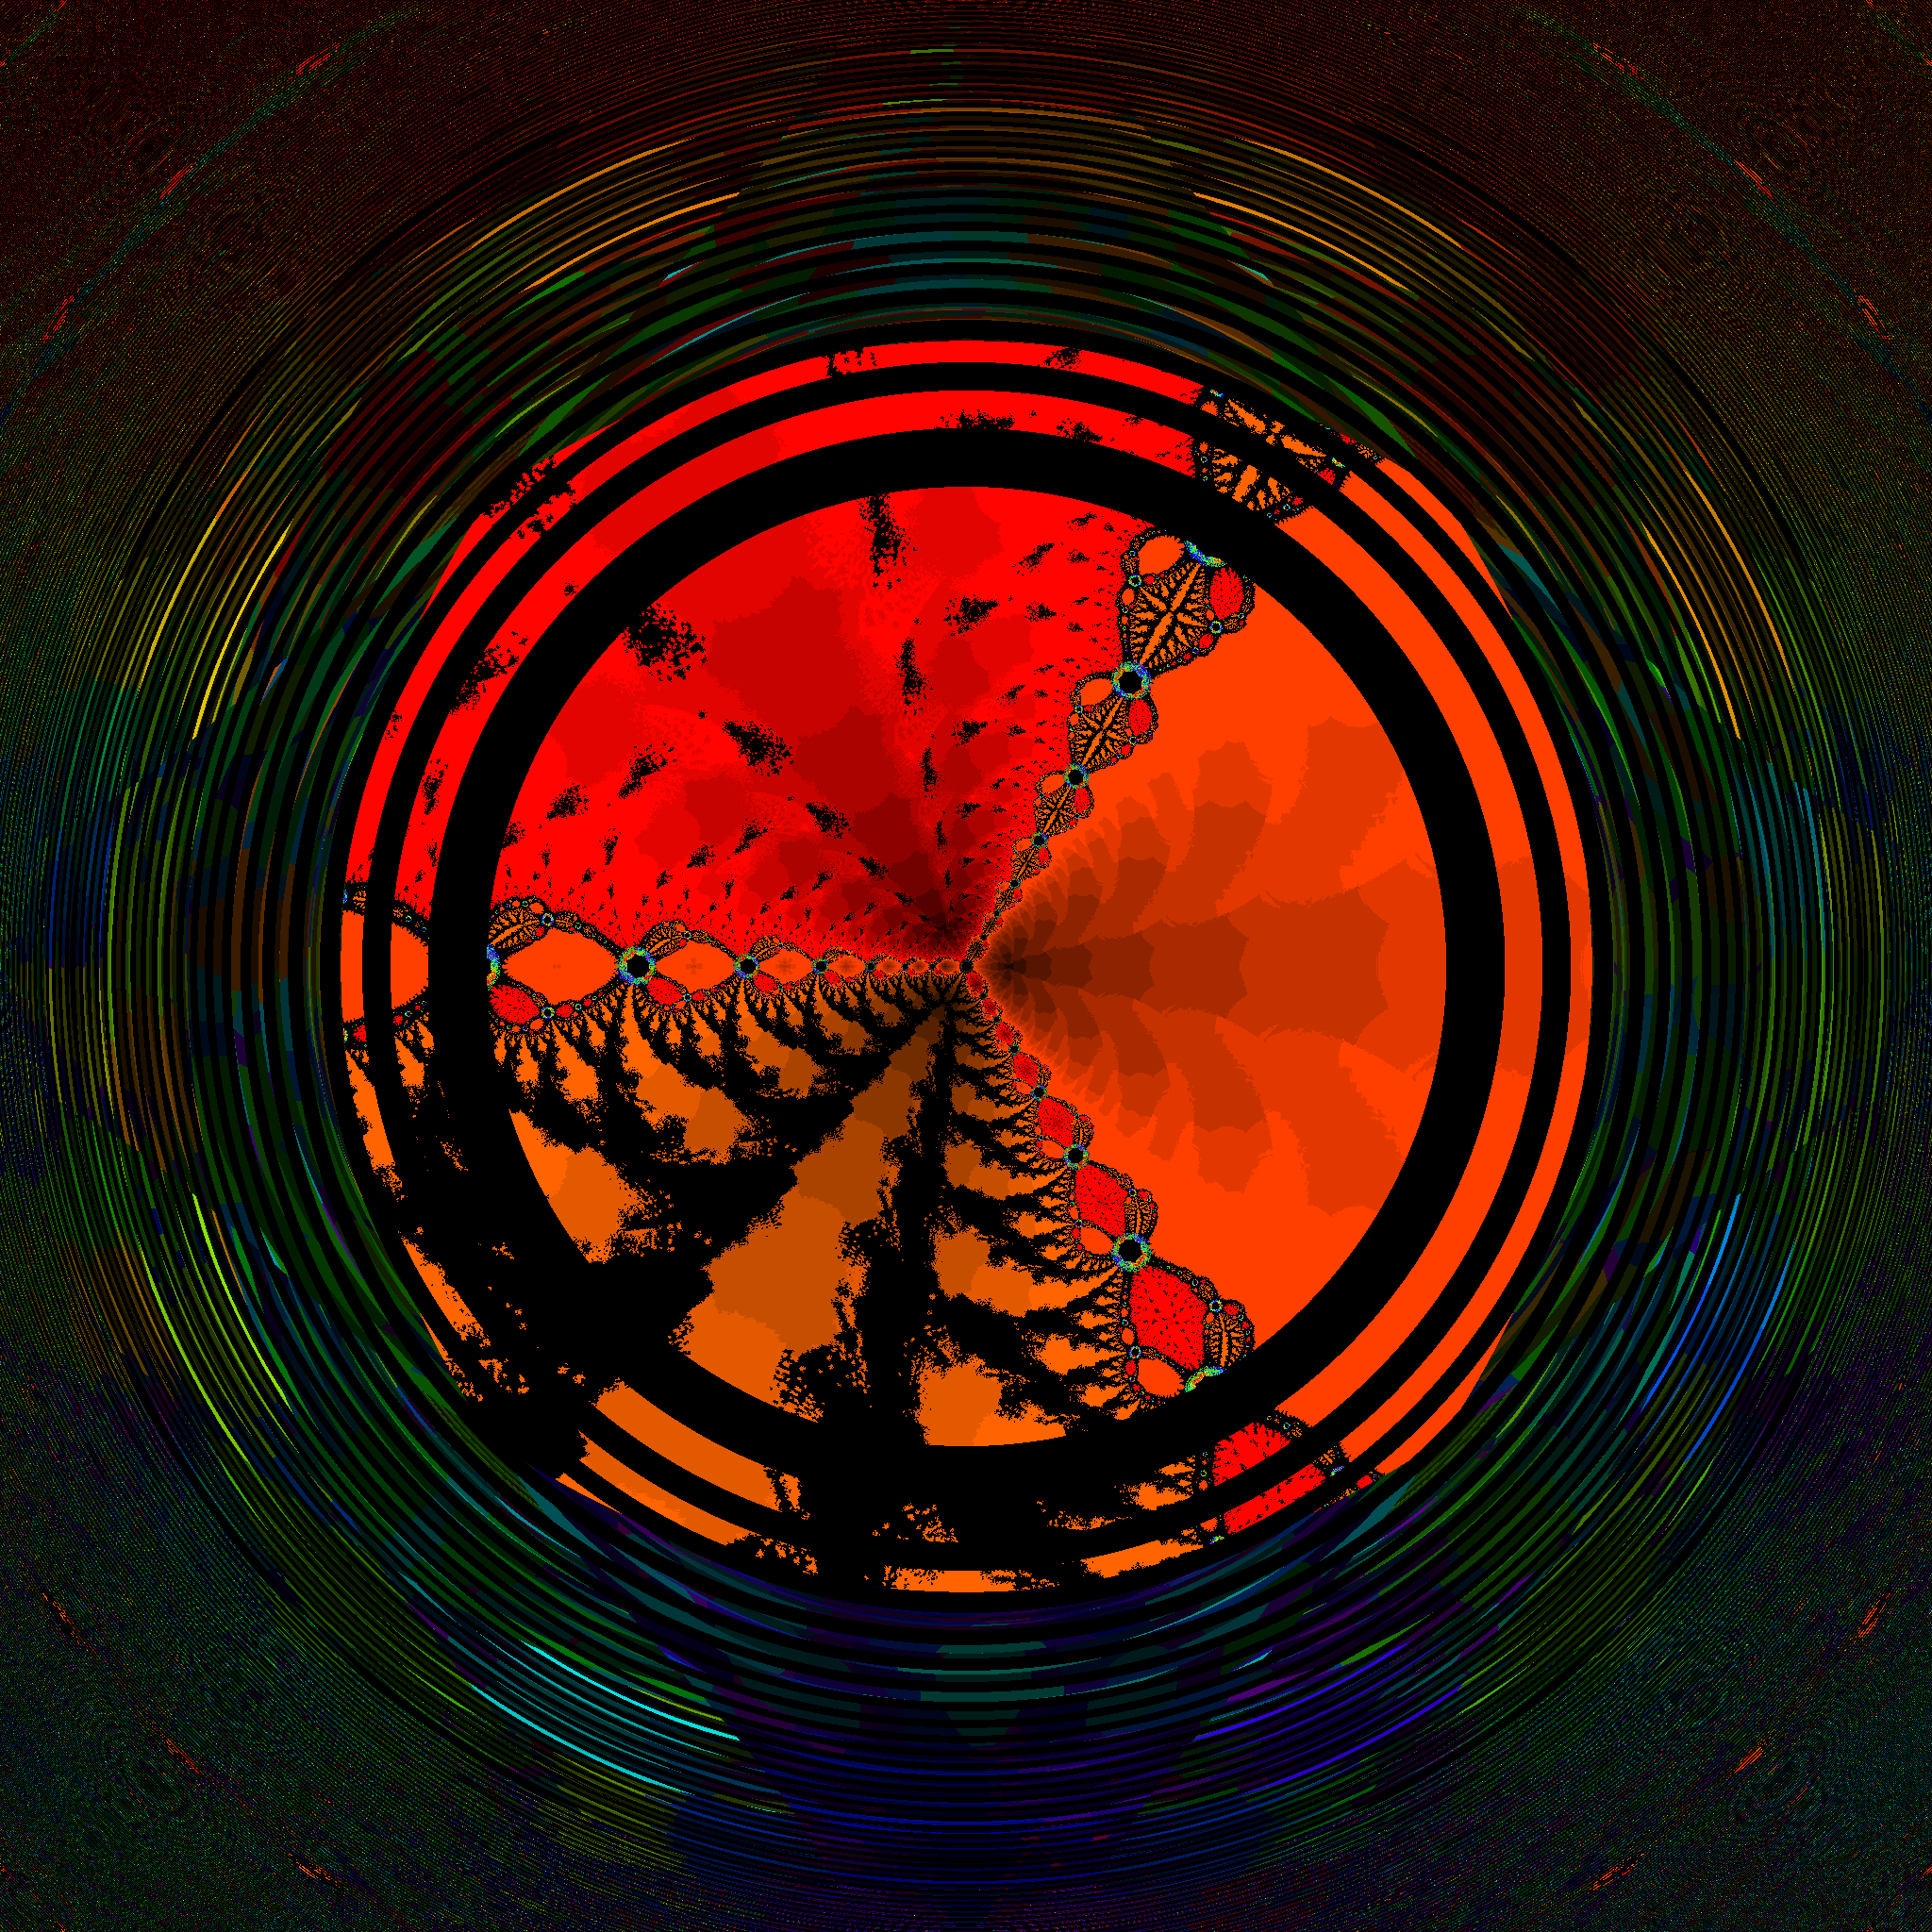
\includegraphics[width=0.23\linewidth]{images/event_horizon/I22F10_horizon.png}
    \end{subfigure}
    \caption{Newton fractal -- outer event horizon (mixed scales)}
    \label{fig:newton-outer-horizon}
\end{figure*}

\begin{figure*}
    \begin{subfigure}[P16]
        \centering
        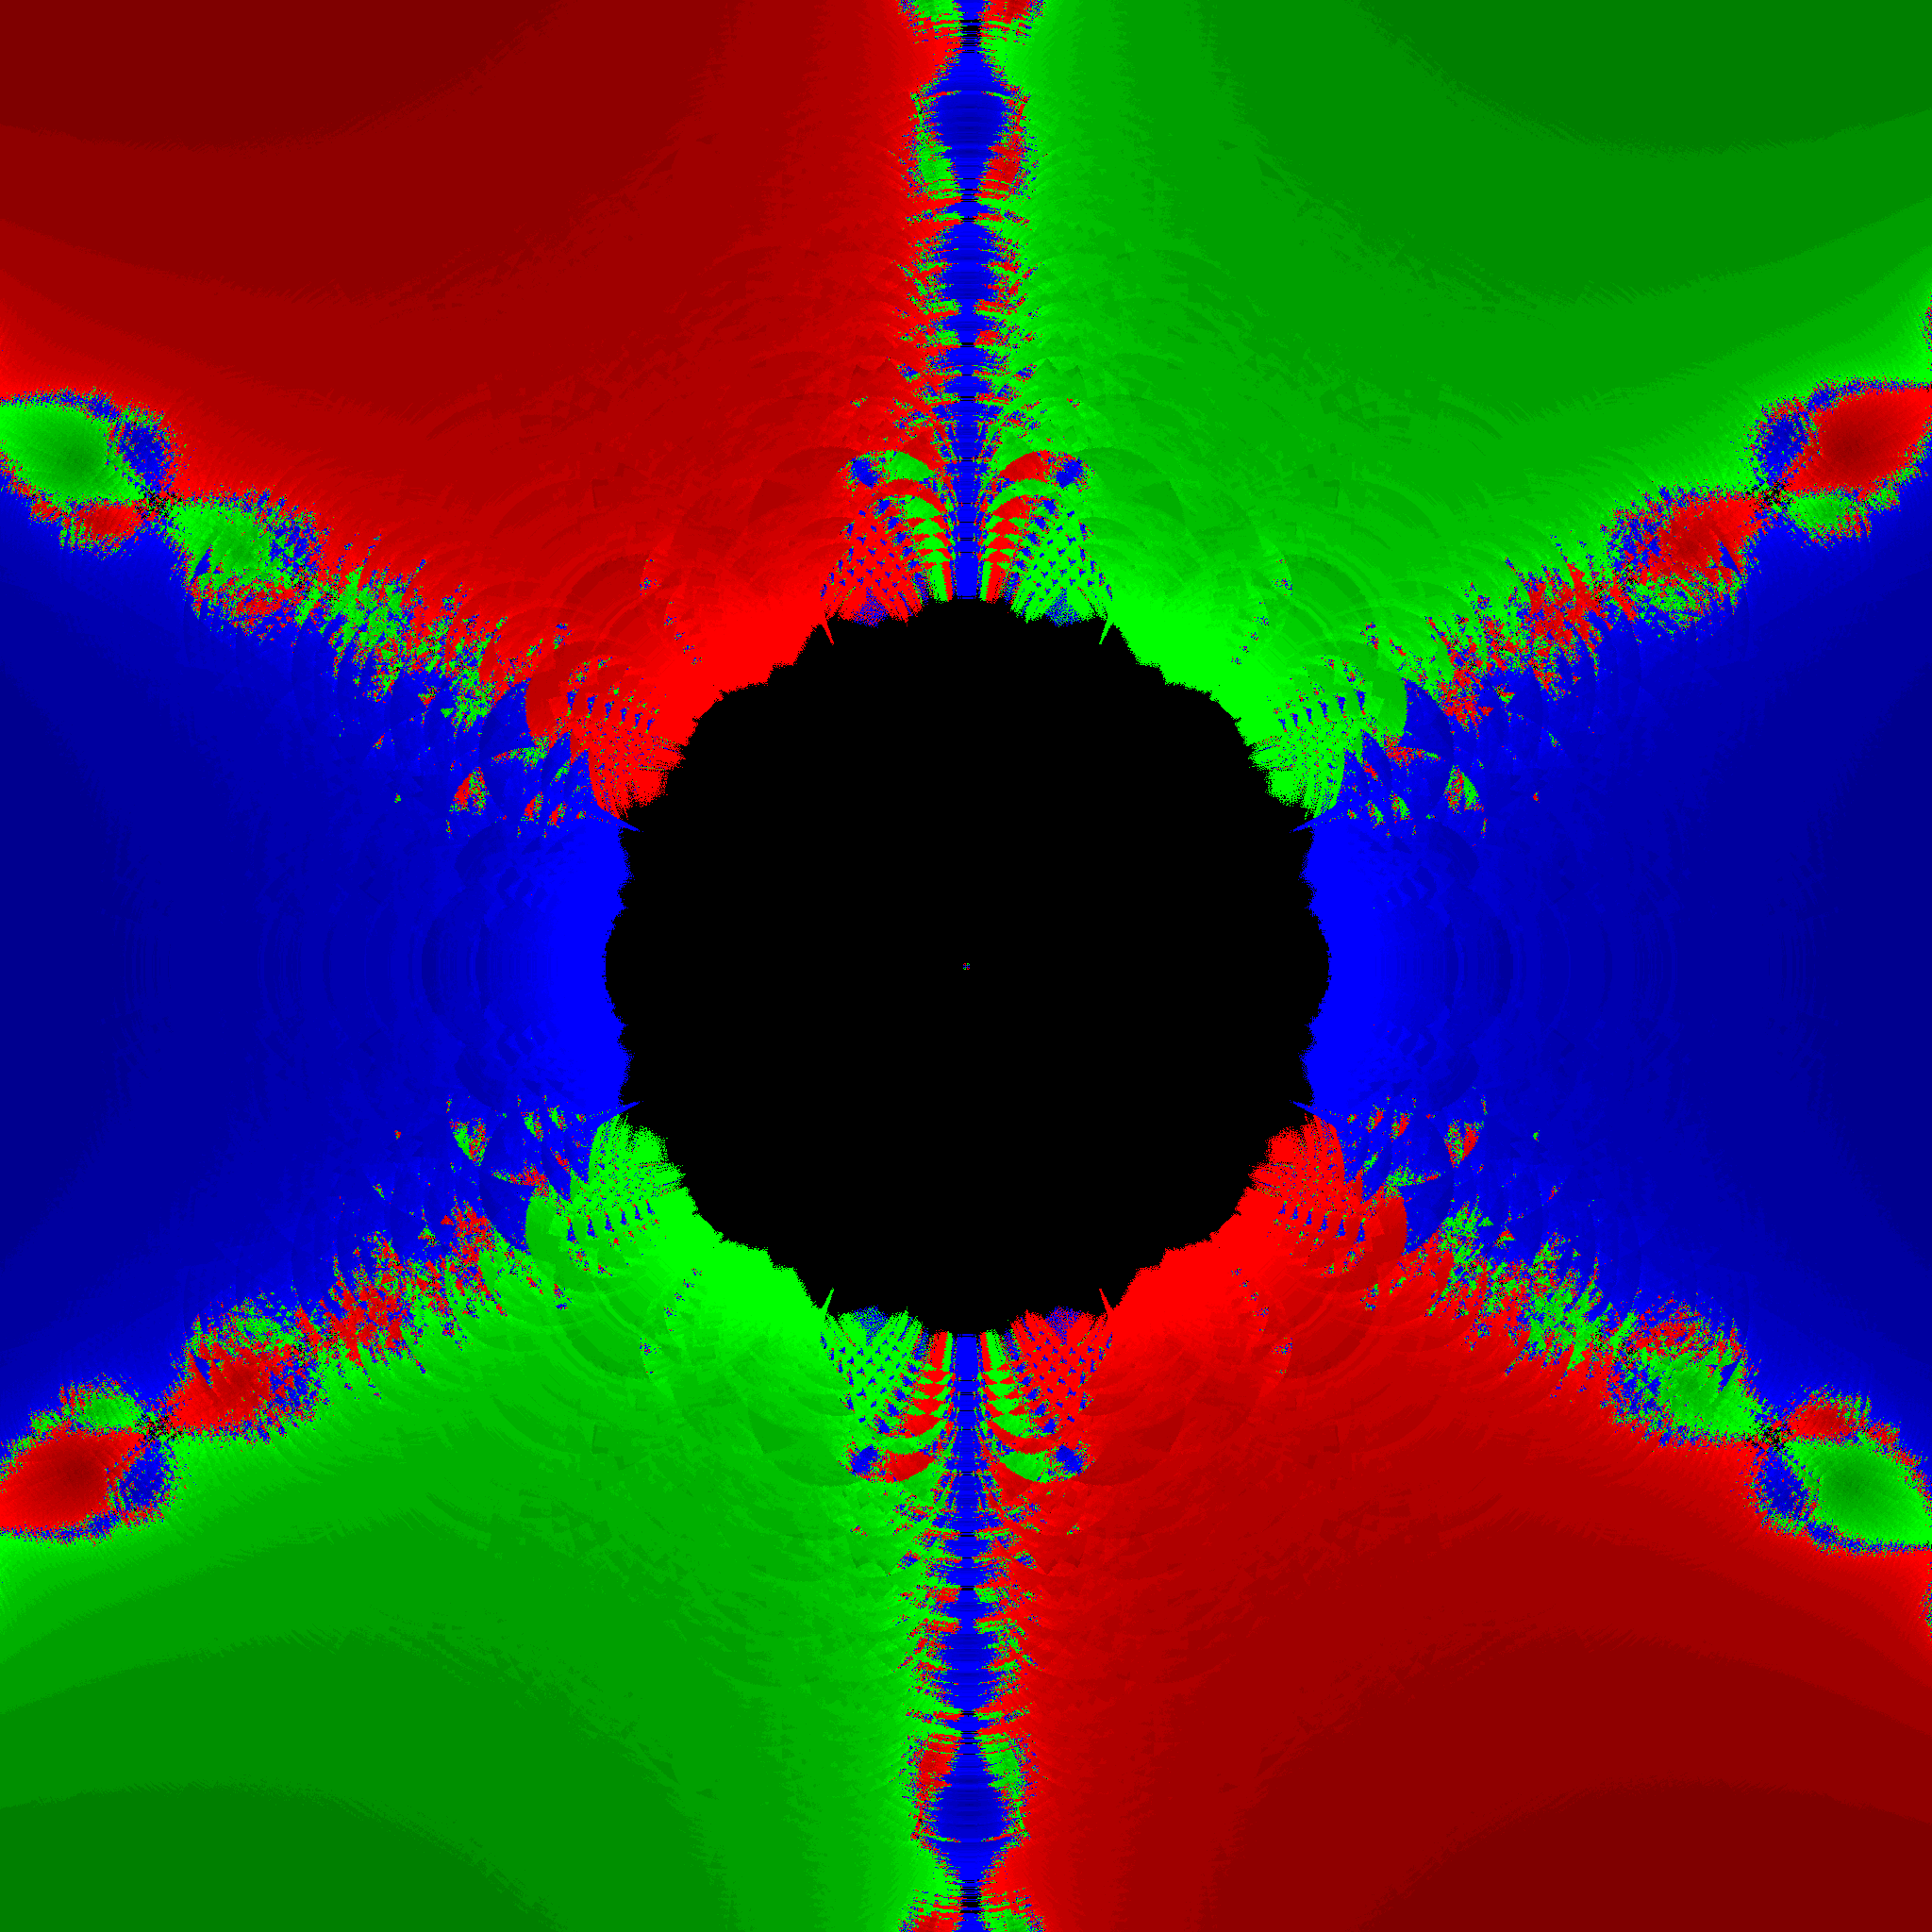
\includegraphics[width=0.31\linewidth]{images/inner_horizon/P16_inner.png}
    \end{subfigure}
    \quad
    \begin{subfigure}[MaskedFloat<4,50>]
        \centering
        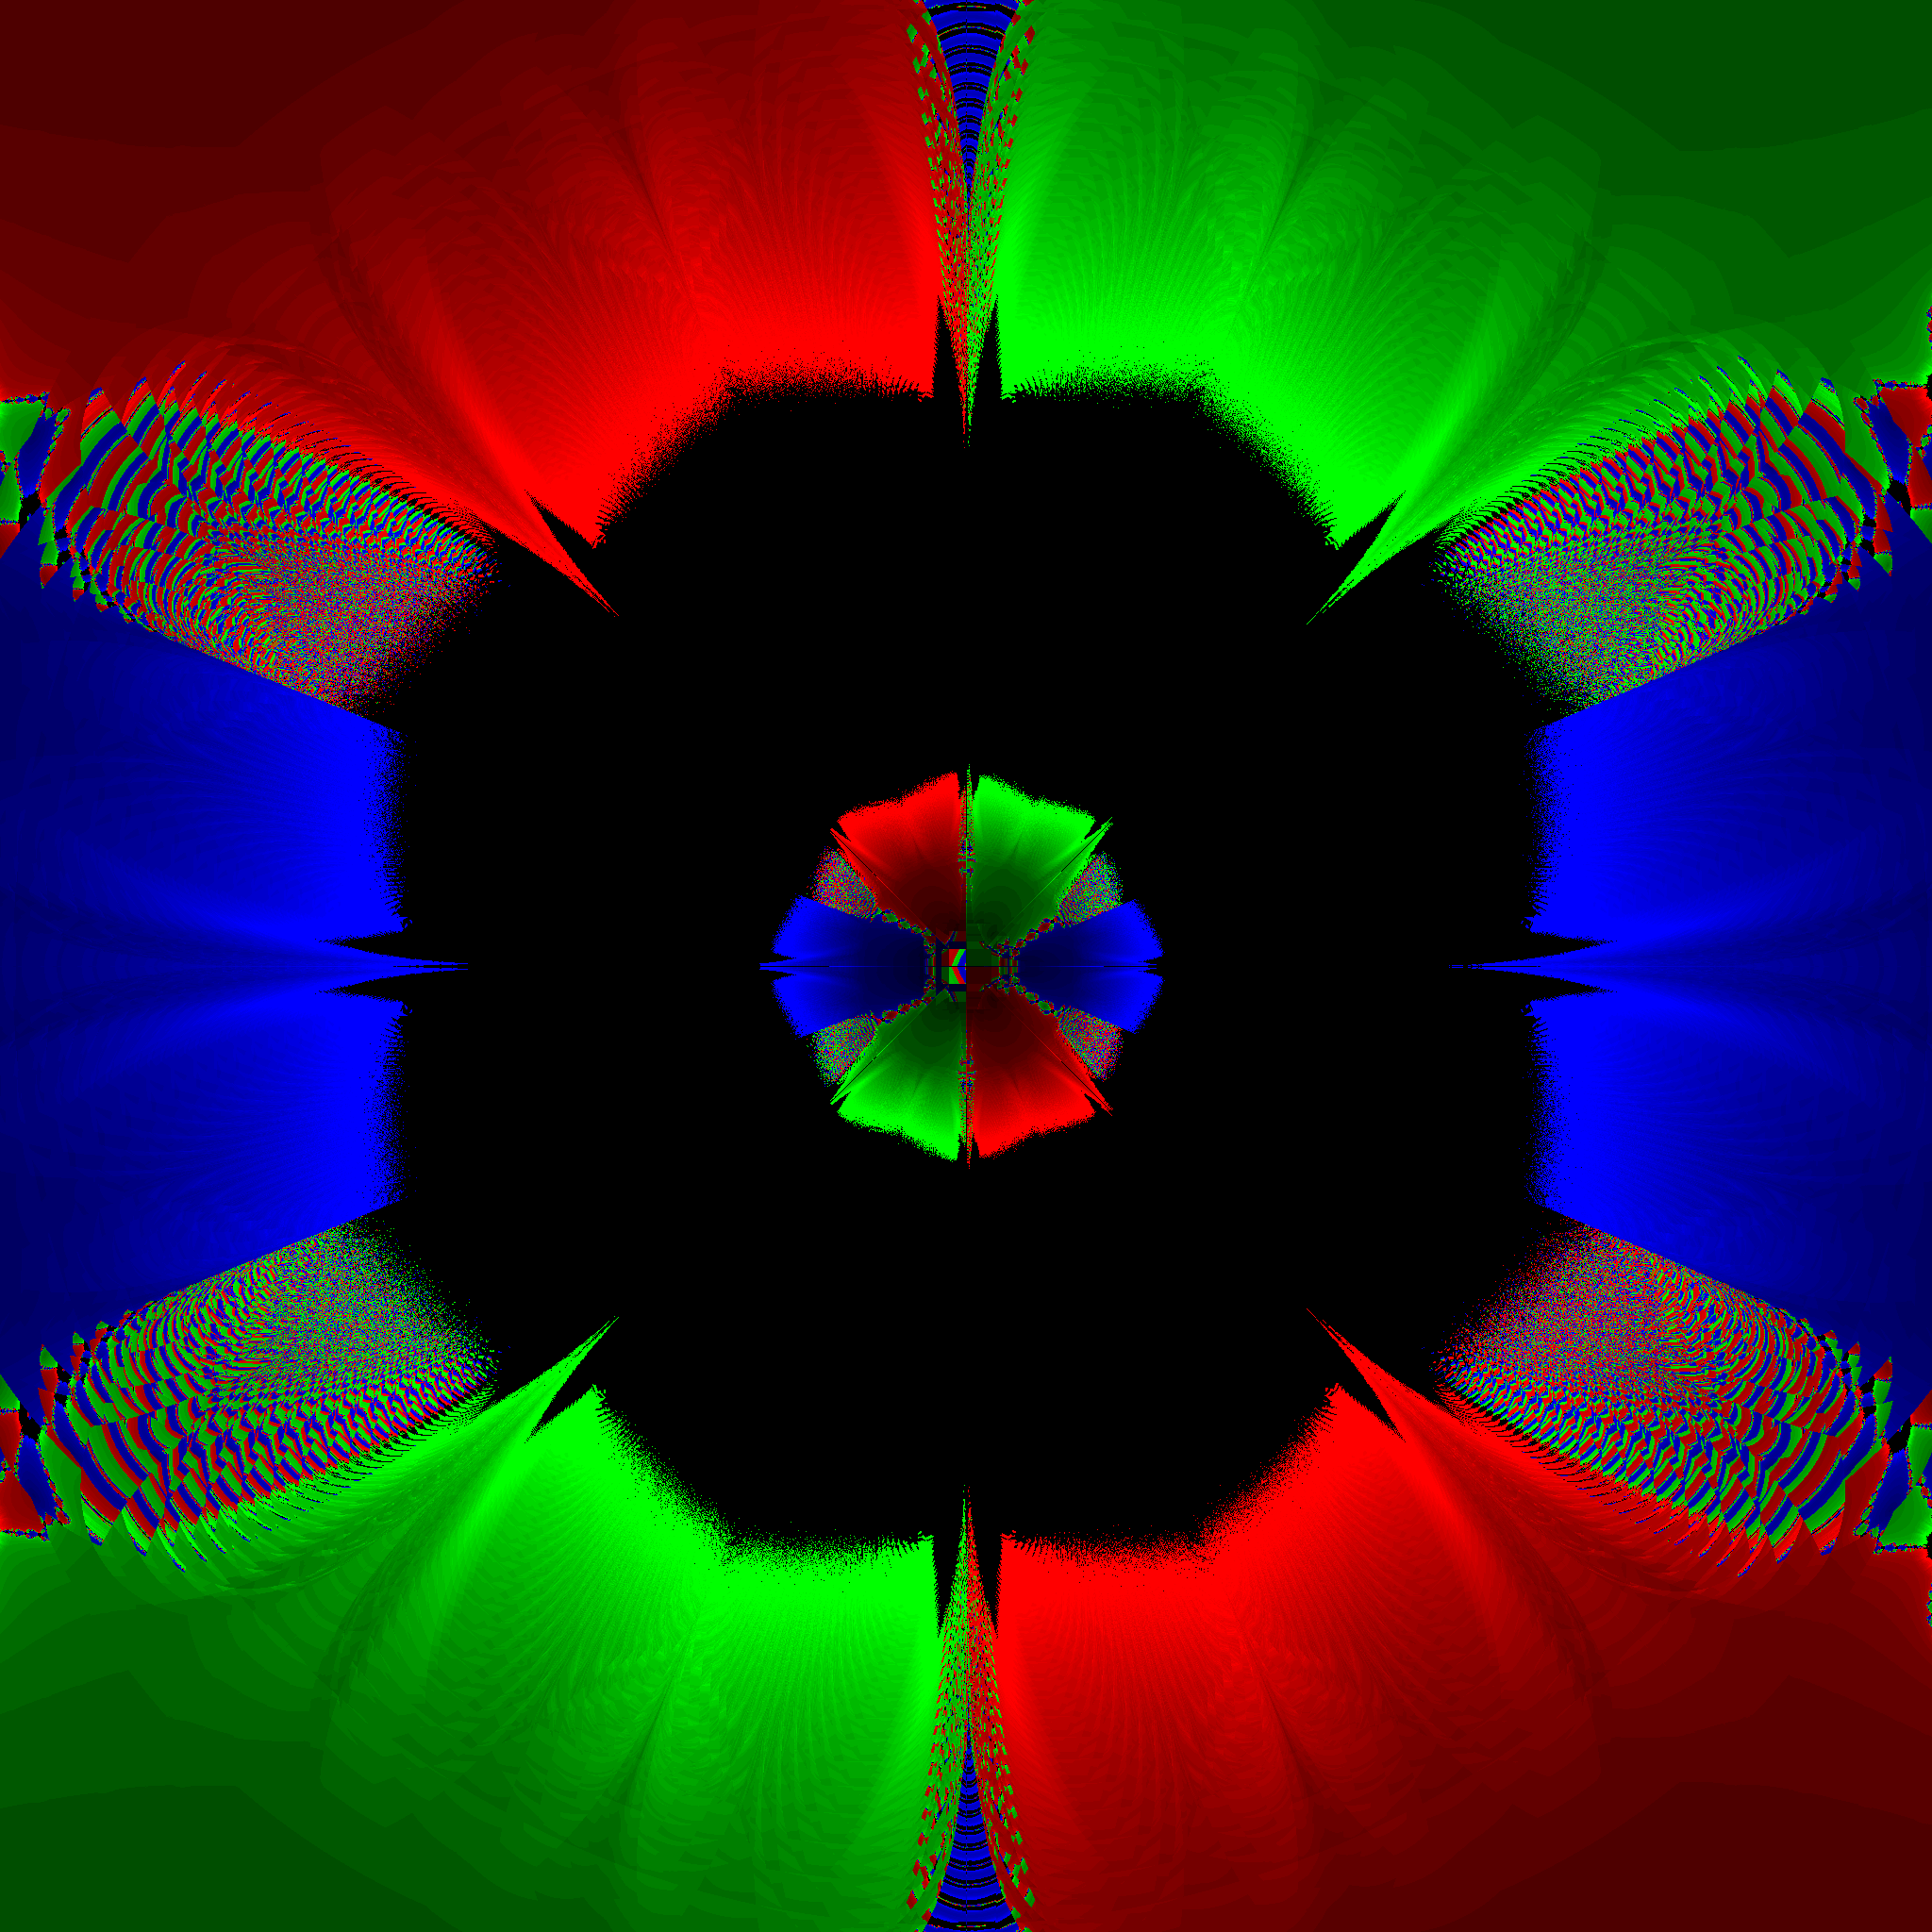
\includegraphics[width=0.31\linewidth]{images/inner_horizon/MaskedFloat_4_50_inner.png}
    \end{subfigure}
    \quad
    \begin{subfigure}[I20F12]
        \centering
        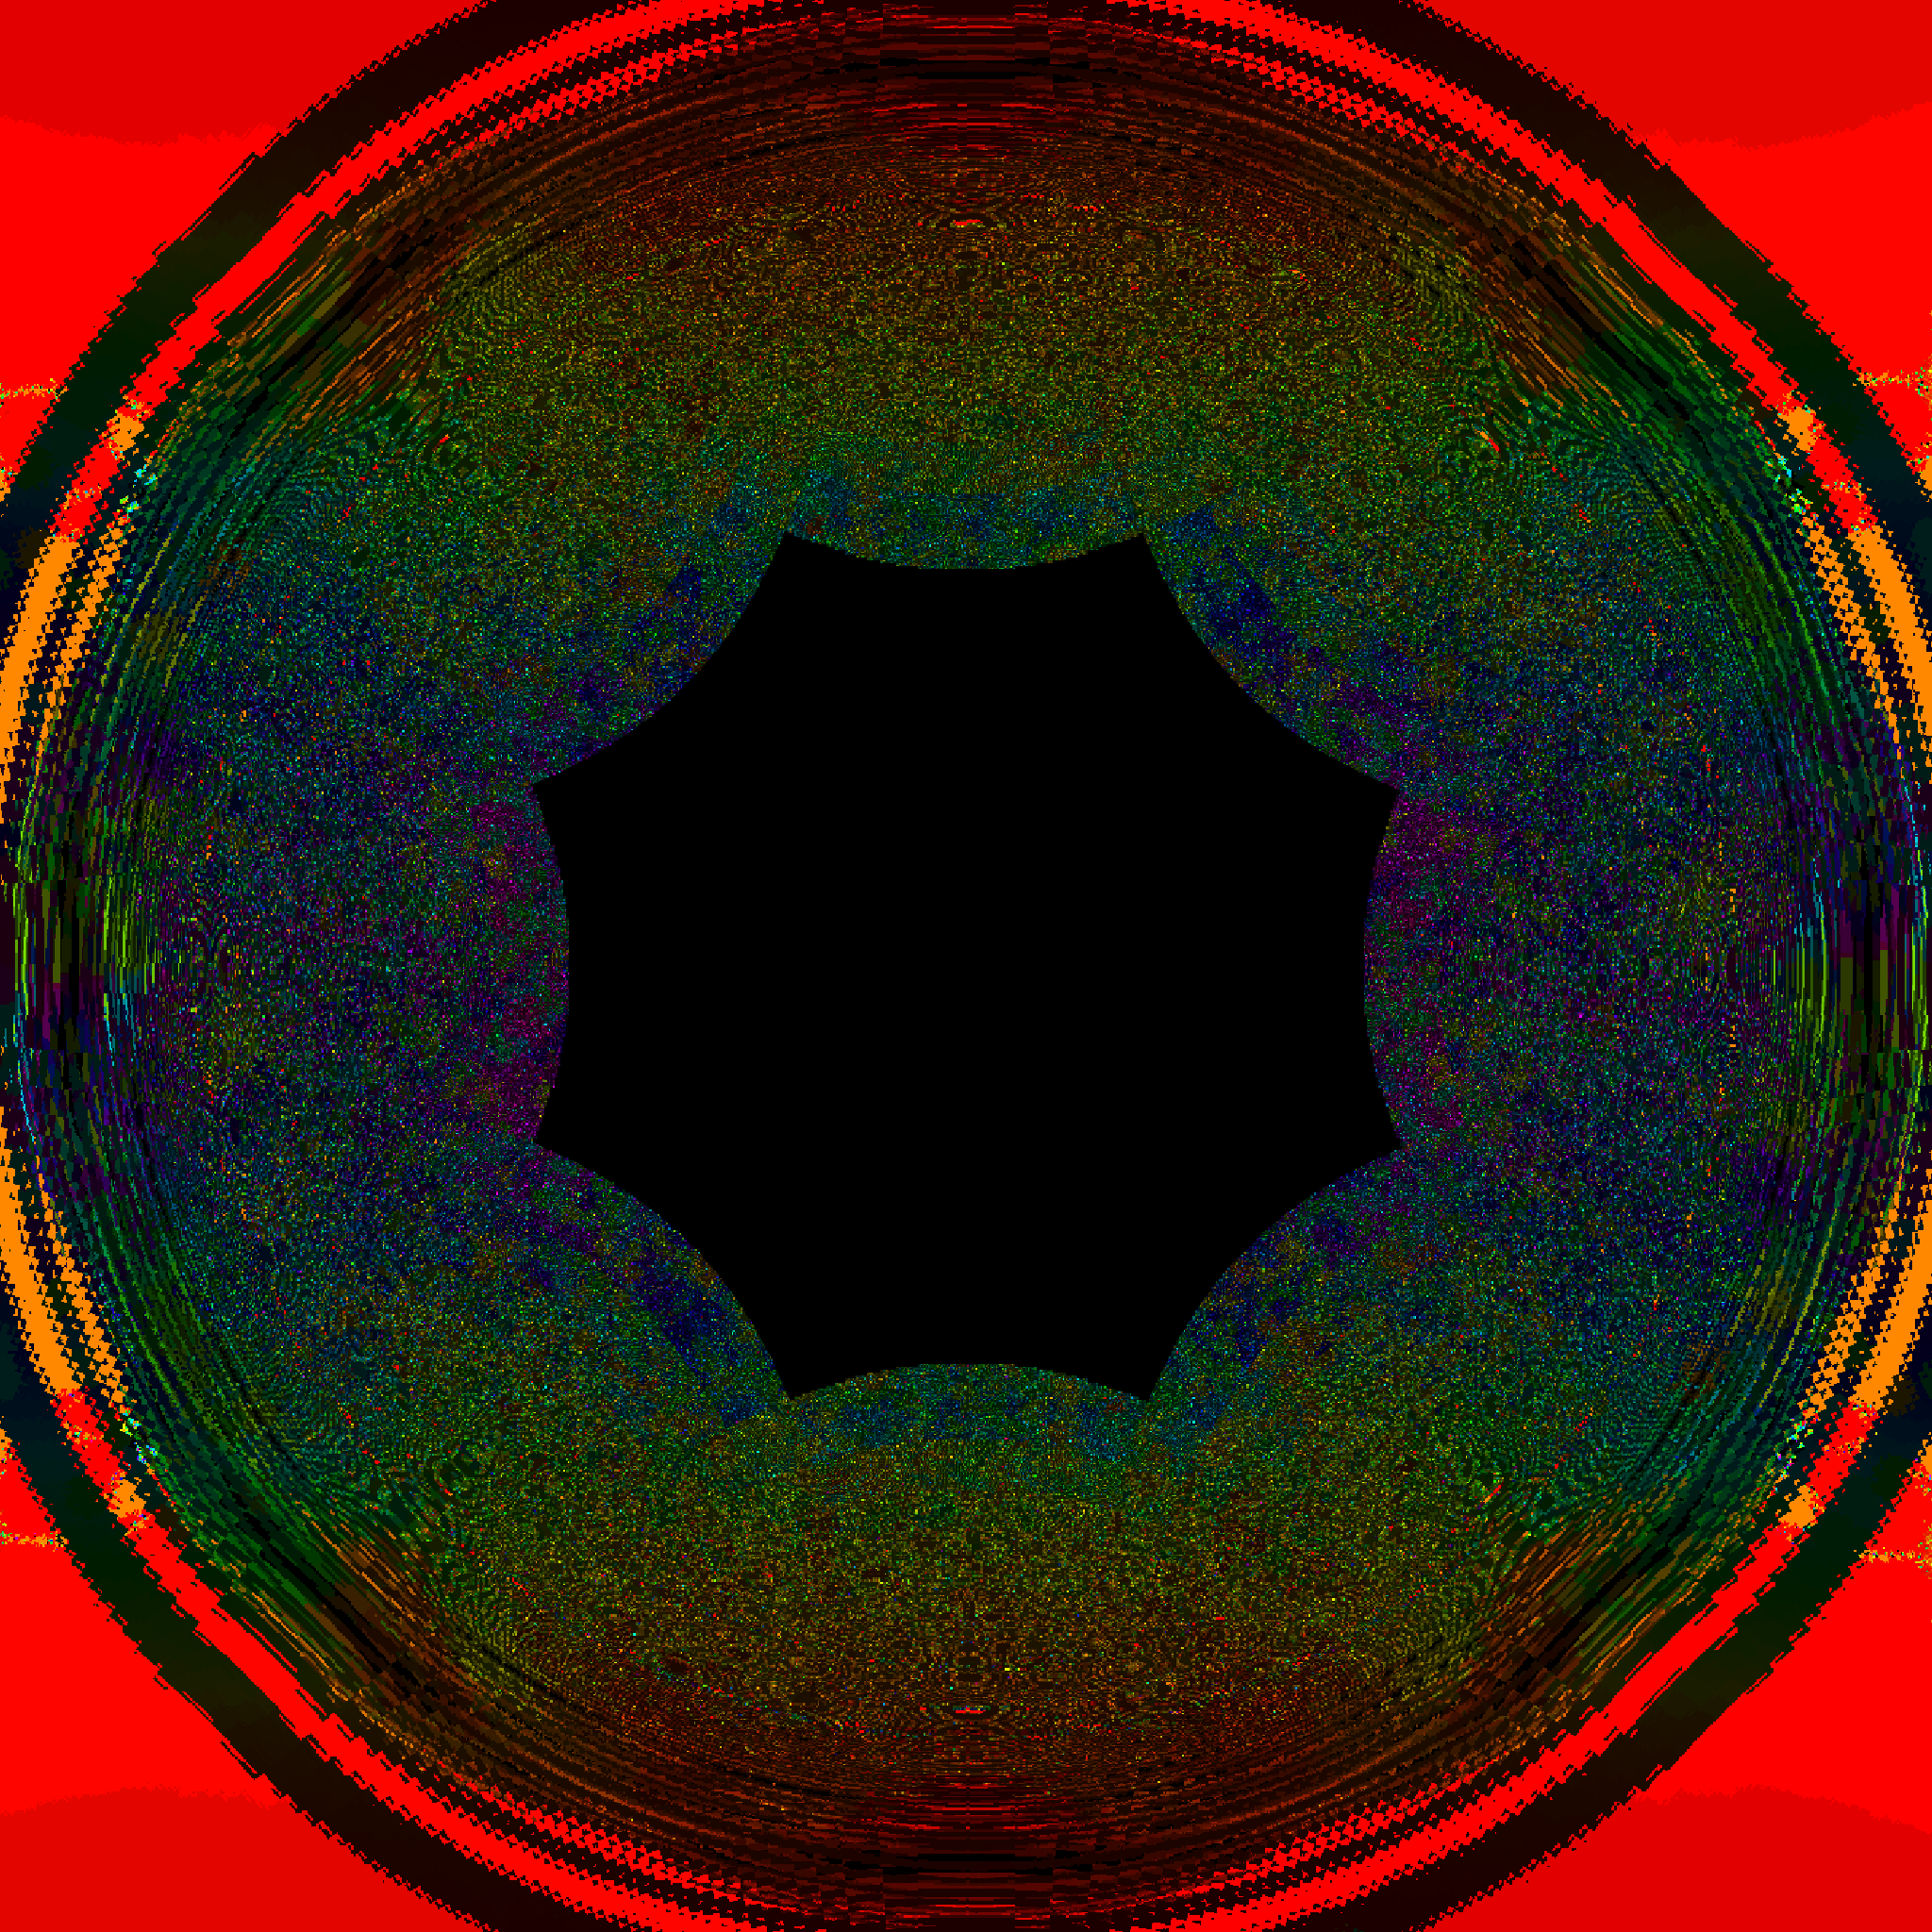
\includegraphics[width=0.31\linewidth]{images/inner_horizon/I20F12_inner.png}
    \end{subfigure}
    \caption{Newton fractal -- inner event horizon}
    \label{fig:newton-inner-horizon}
\end{figure*}

As you zoom farther out in the Newton fractal, we reach the point where the formats can no longer 
store the values of the starting position or its intermediate
values (or can only store with reduced accuracy). The authors refer to this as the outer event horizon. 
Figure \ref{fig:newton-outer-horizon},
shows the shape of this event horizon for various types. Note that these are not at the same 
zoom level--\texttt{f32} can represent much, much larger numbers than the others. 

If instead of zooming out towards infinity, we zoom in towards zero, we reach the
inner event horizon--where the formats cannot represent how small the numbers have become.
Figure \ref{fig:newton-inner-horizon} shows the shapes and edges of this inner
event horizon. Interestingly, the inner event horizon appears at approximately the
same scale for \texttt{P16}, \texttt{MaskedFloat<4,50>}, and \texttt{I20F12}; Figure \ref{fig:newton-inner-horizon} depicts a consistent scale.

\begin{figure*}
    \begin{subfigure}[P16]
        \centering
        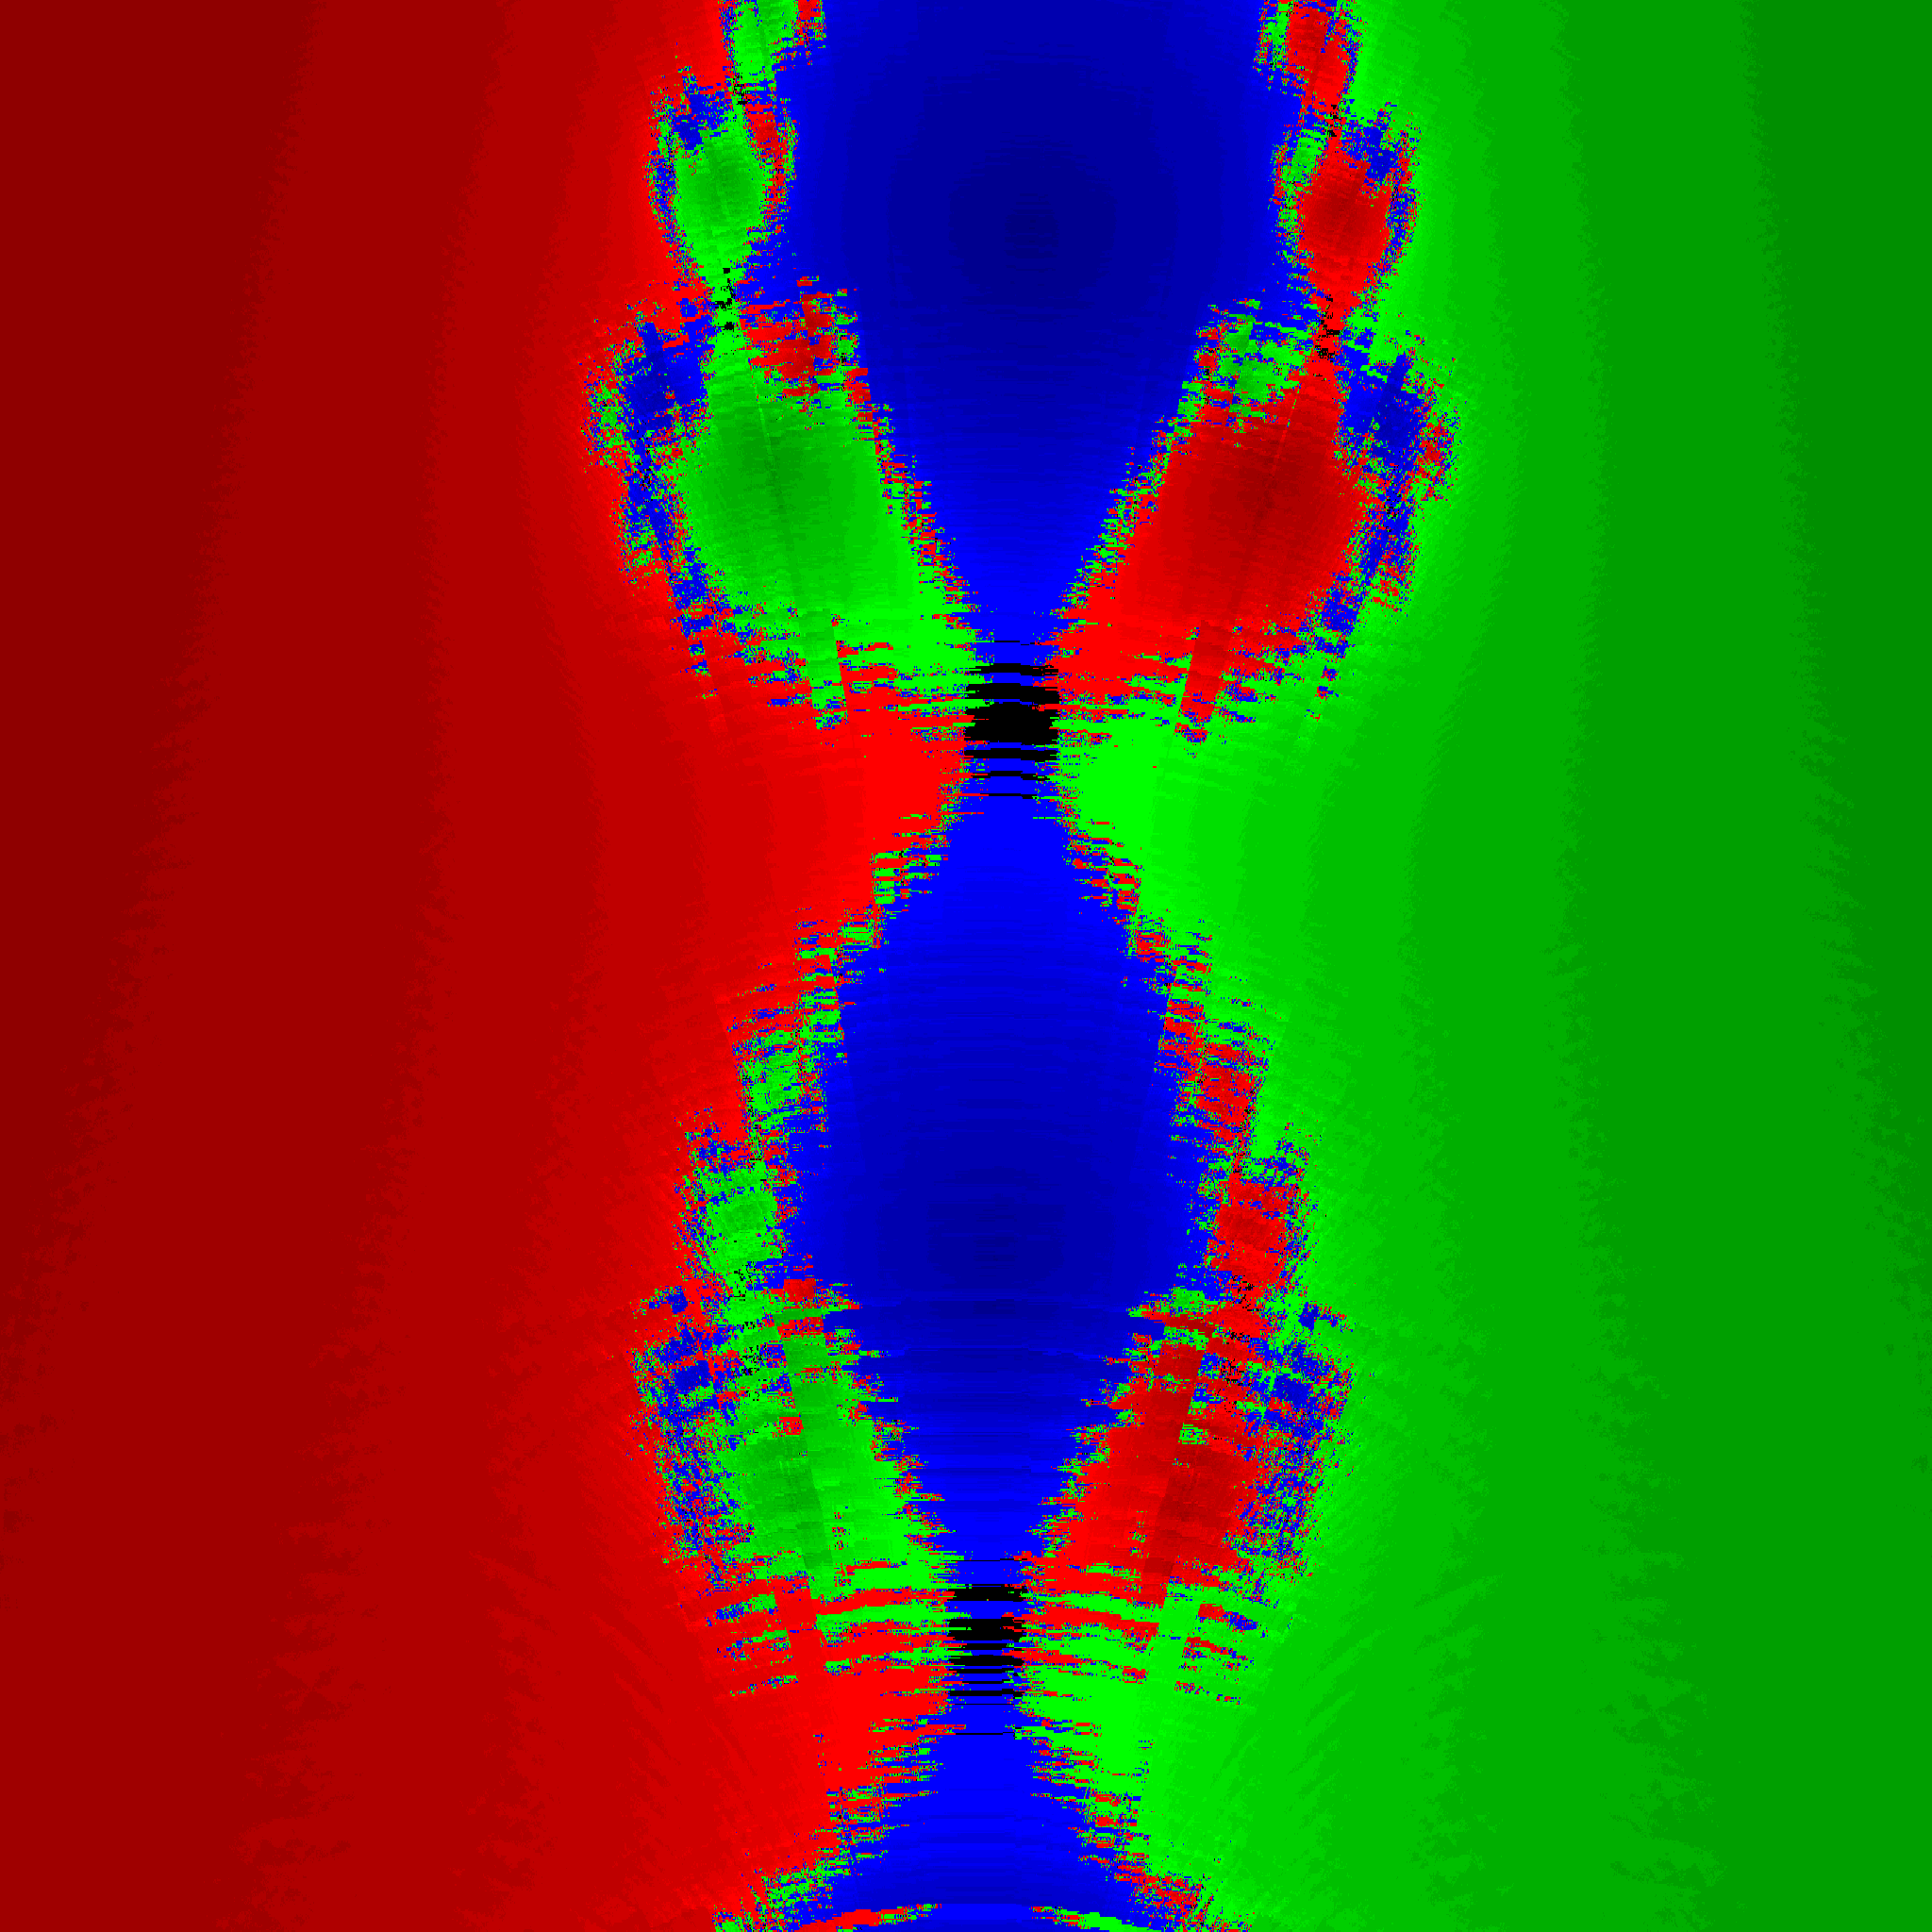
\includegraphics[width=0.30\linewidth]{images/near_horizon/P16_near.png}
    \end{subfigure}
    \quad
    \begin{subfigure}[MaskedFloat<4,50>]
        \centering
        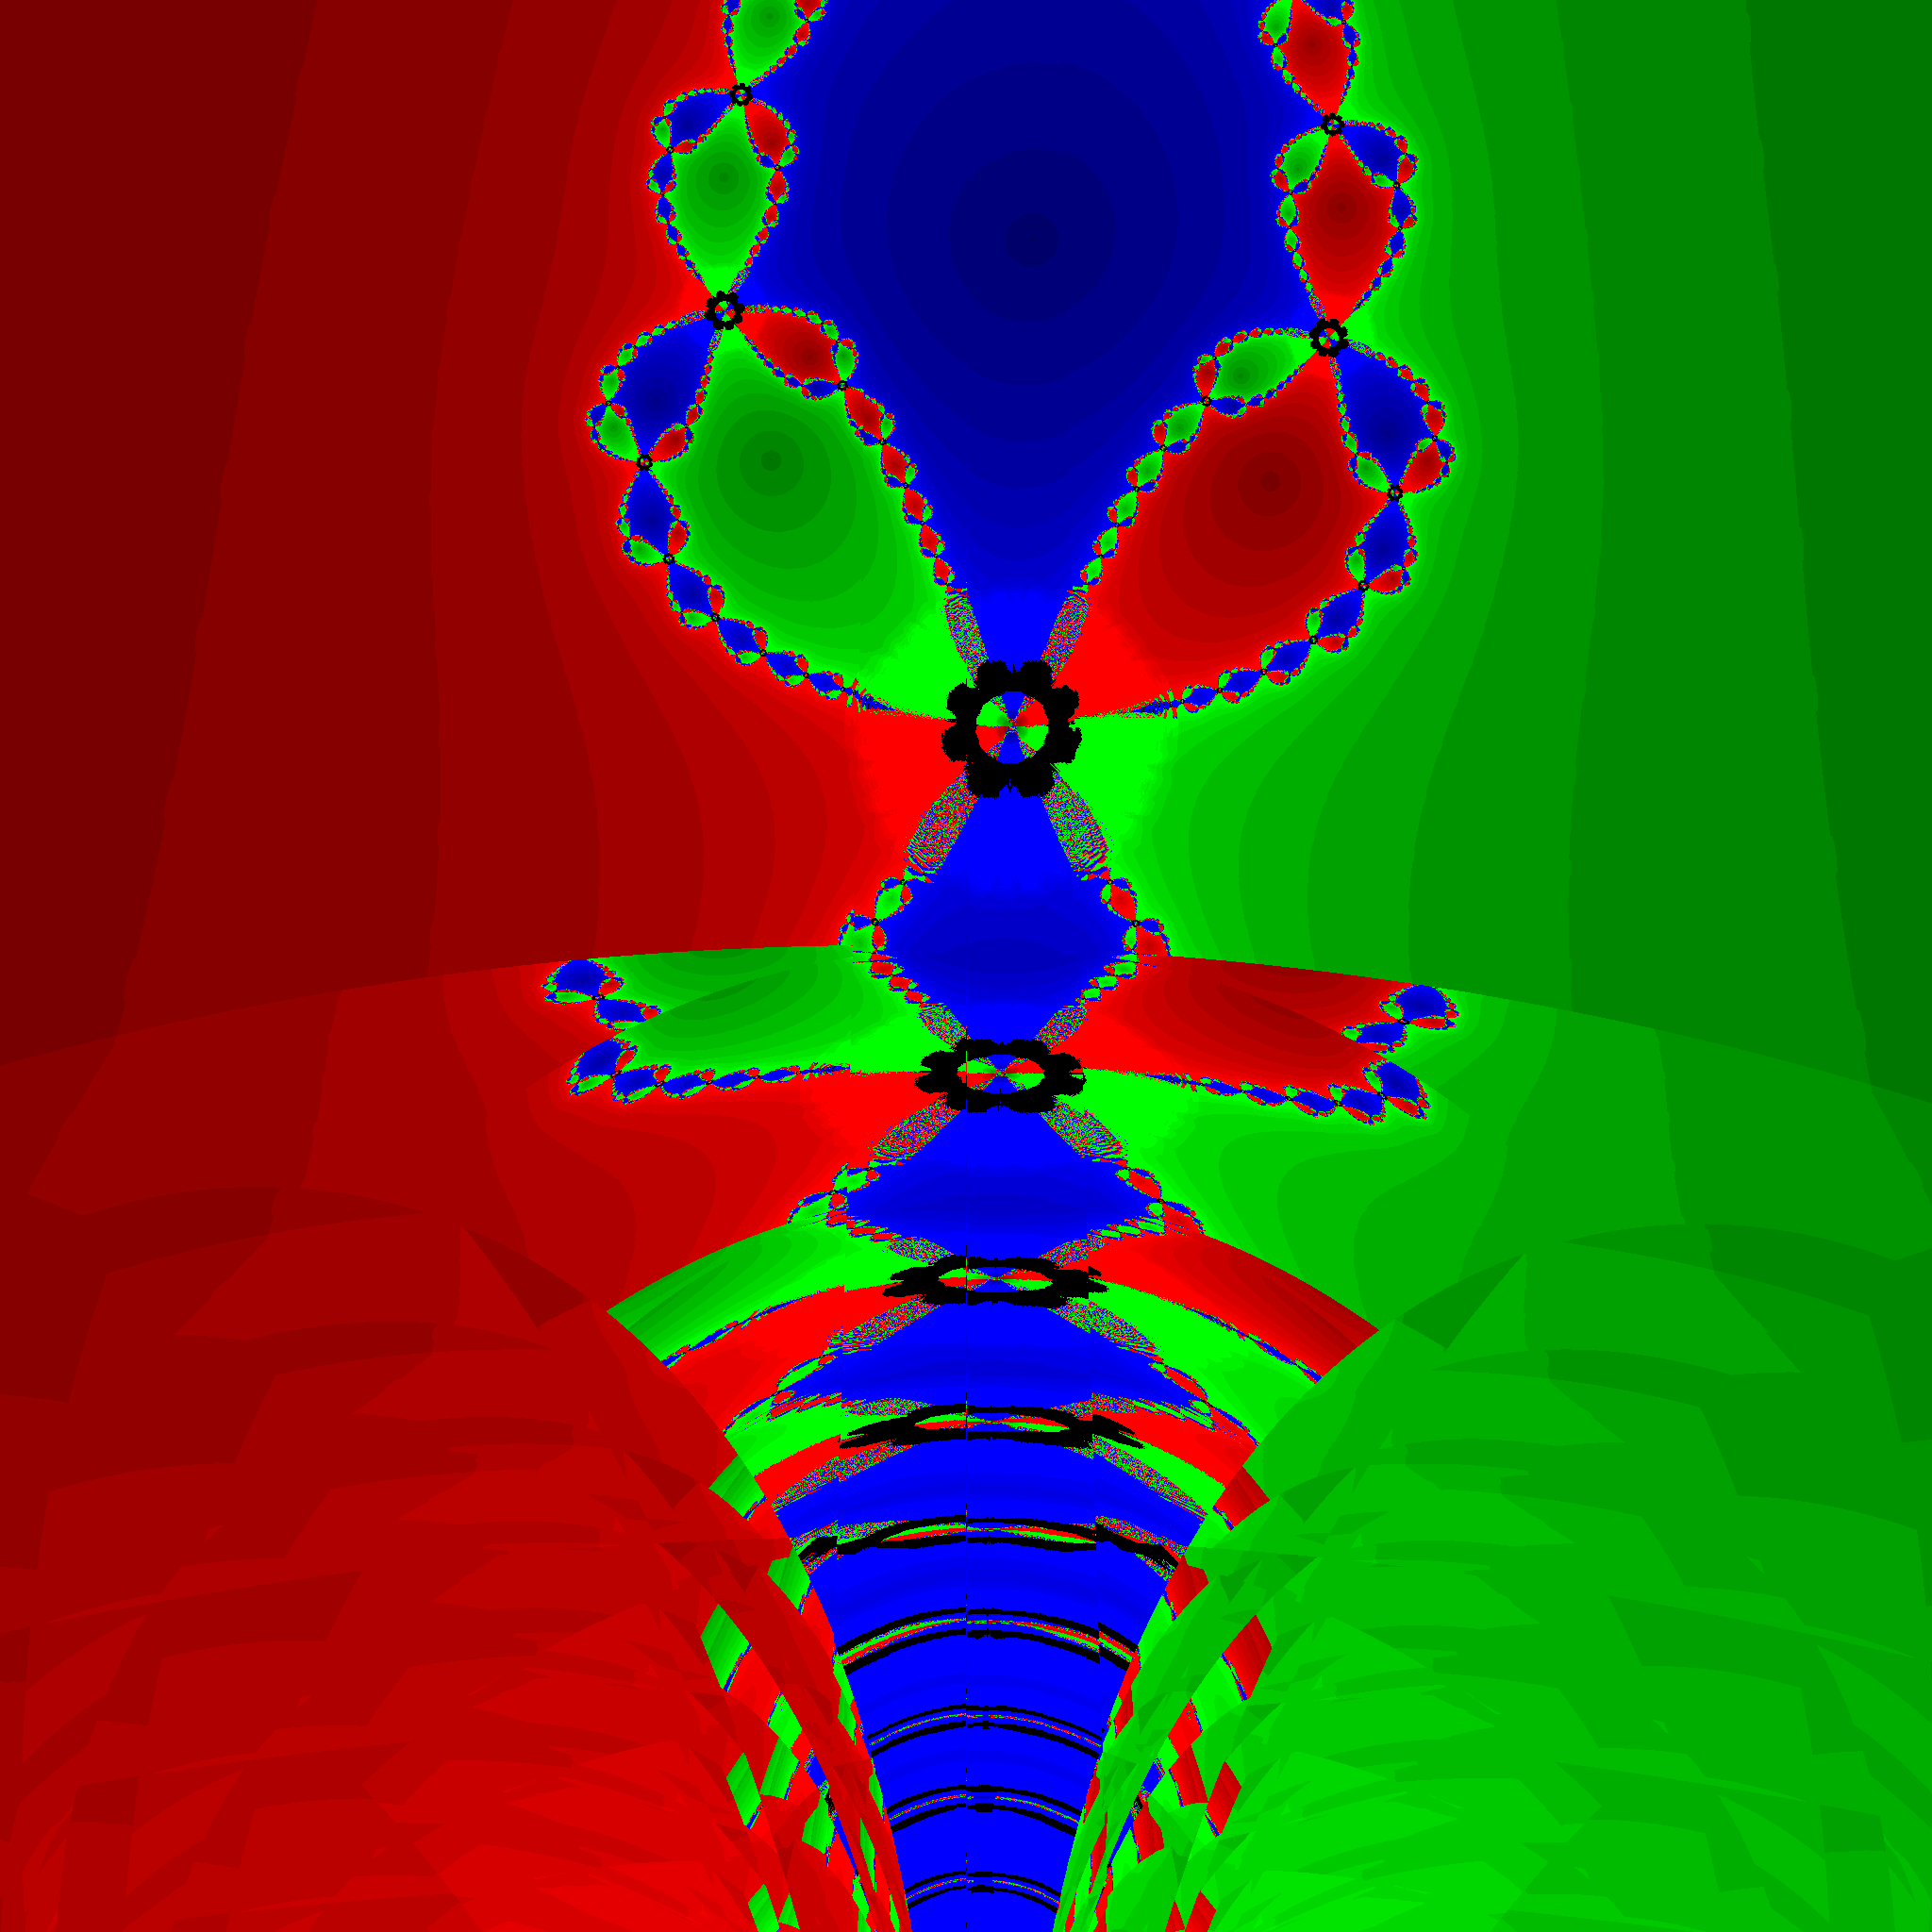
\includegraphics[width=0.30\linewidth]{images/near_horizon/MaskedFloat_450_near.png}
    \end{subfigure}
    \quad
    \begin{subfigure}[I20F12]
        \centering
        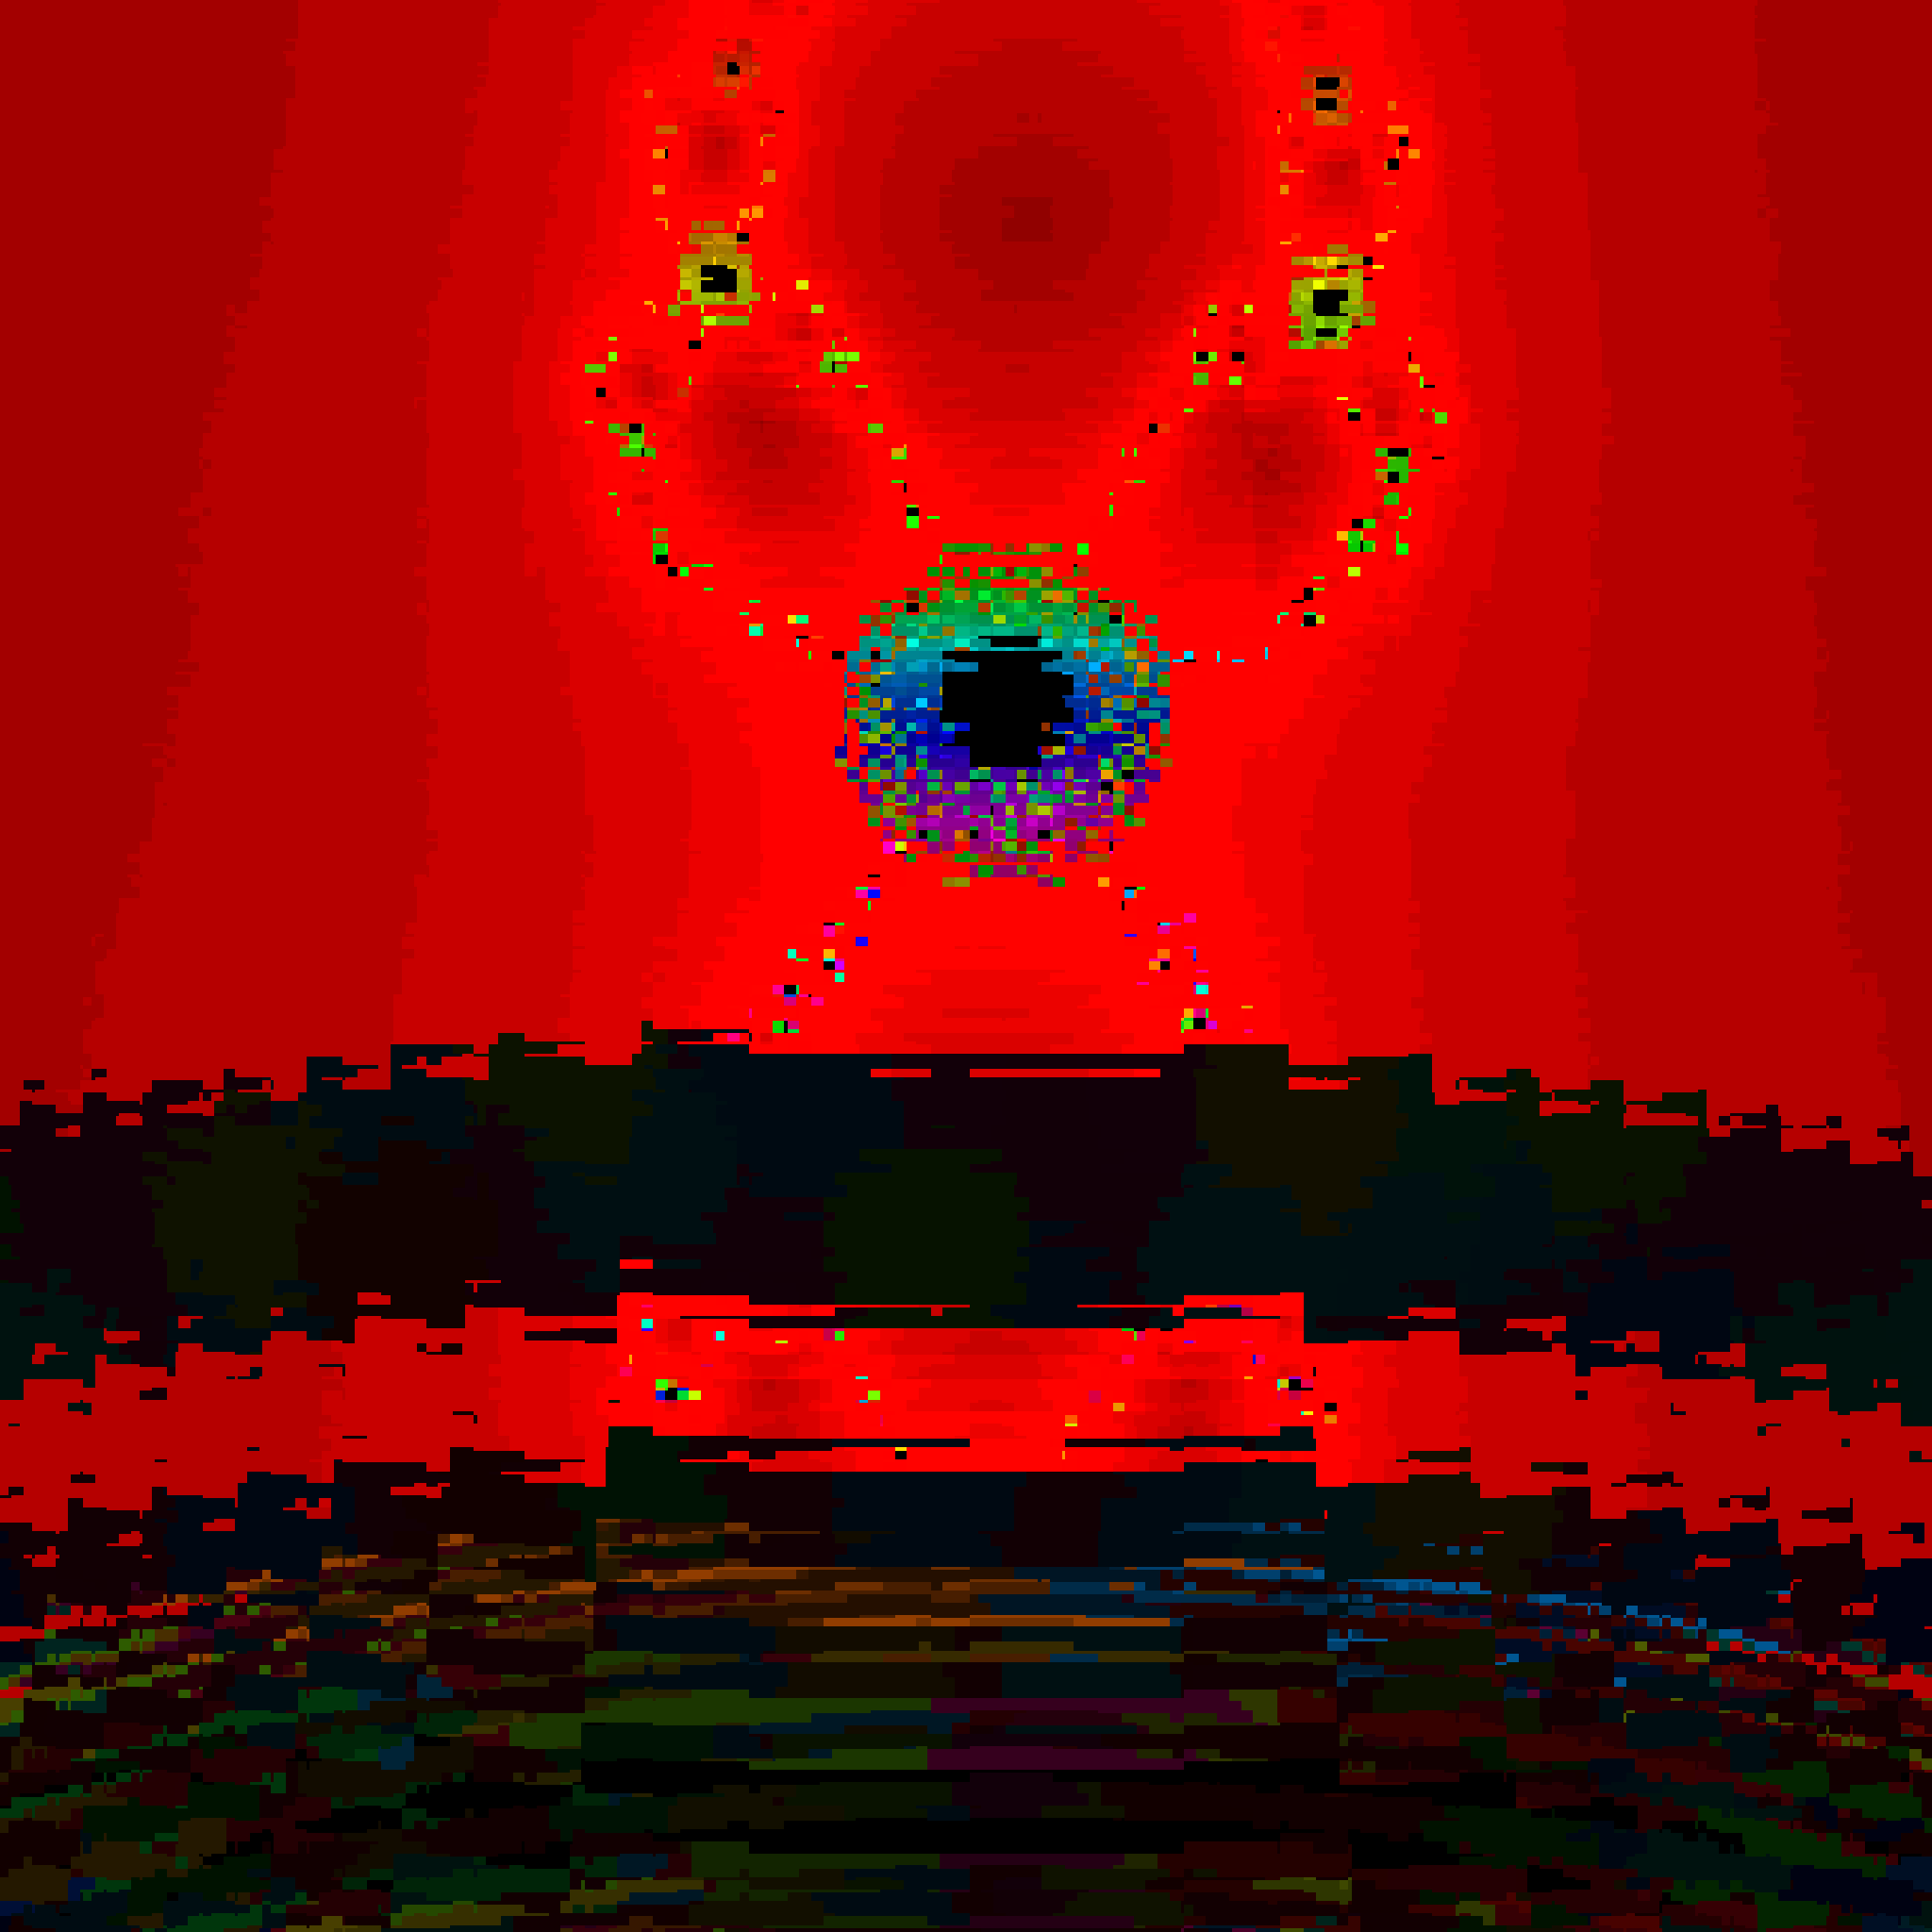
\includegraphics[width=0.30\linewidth]{images/near_horizon/I20F12_near.png}
    \end{subfigure}
    \caption{Near the inner Newton event horizon}
    \label{fig:newton-near-horizon}
\end{figure*}

Slightly above the inner event horizon, there's also an interesting distortion region, 
where the intermediate values get twisted and warped at the edge of their range.
See Figure \ref{fig:newton-near-horizon} for some examples, from the wobbly 
\texttt{P16}, to the
funhouse mirror of MaskedFloat, and lastly a demonic sunrise over \texttt{I20F12}.

%% /newton/?x=0&y=0&window=2916&scale=64&res=512&iters=16
%% /newton/?x=0&y=-720&window=288&scale=3645&res=512&iters=64 
%% newton/?x=0&y=0&window=6561&scale=64&res=2048&iters=64
%% newton/?x=0&y=0&window=207546875&scale=2&res=2048&iters=200

\begin{figure}
    \begin{subfigure}[MaskedFloat<4,50>]
        \centering
        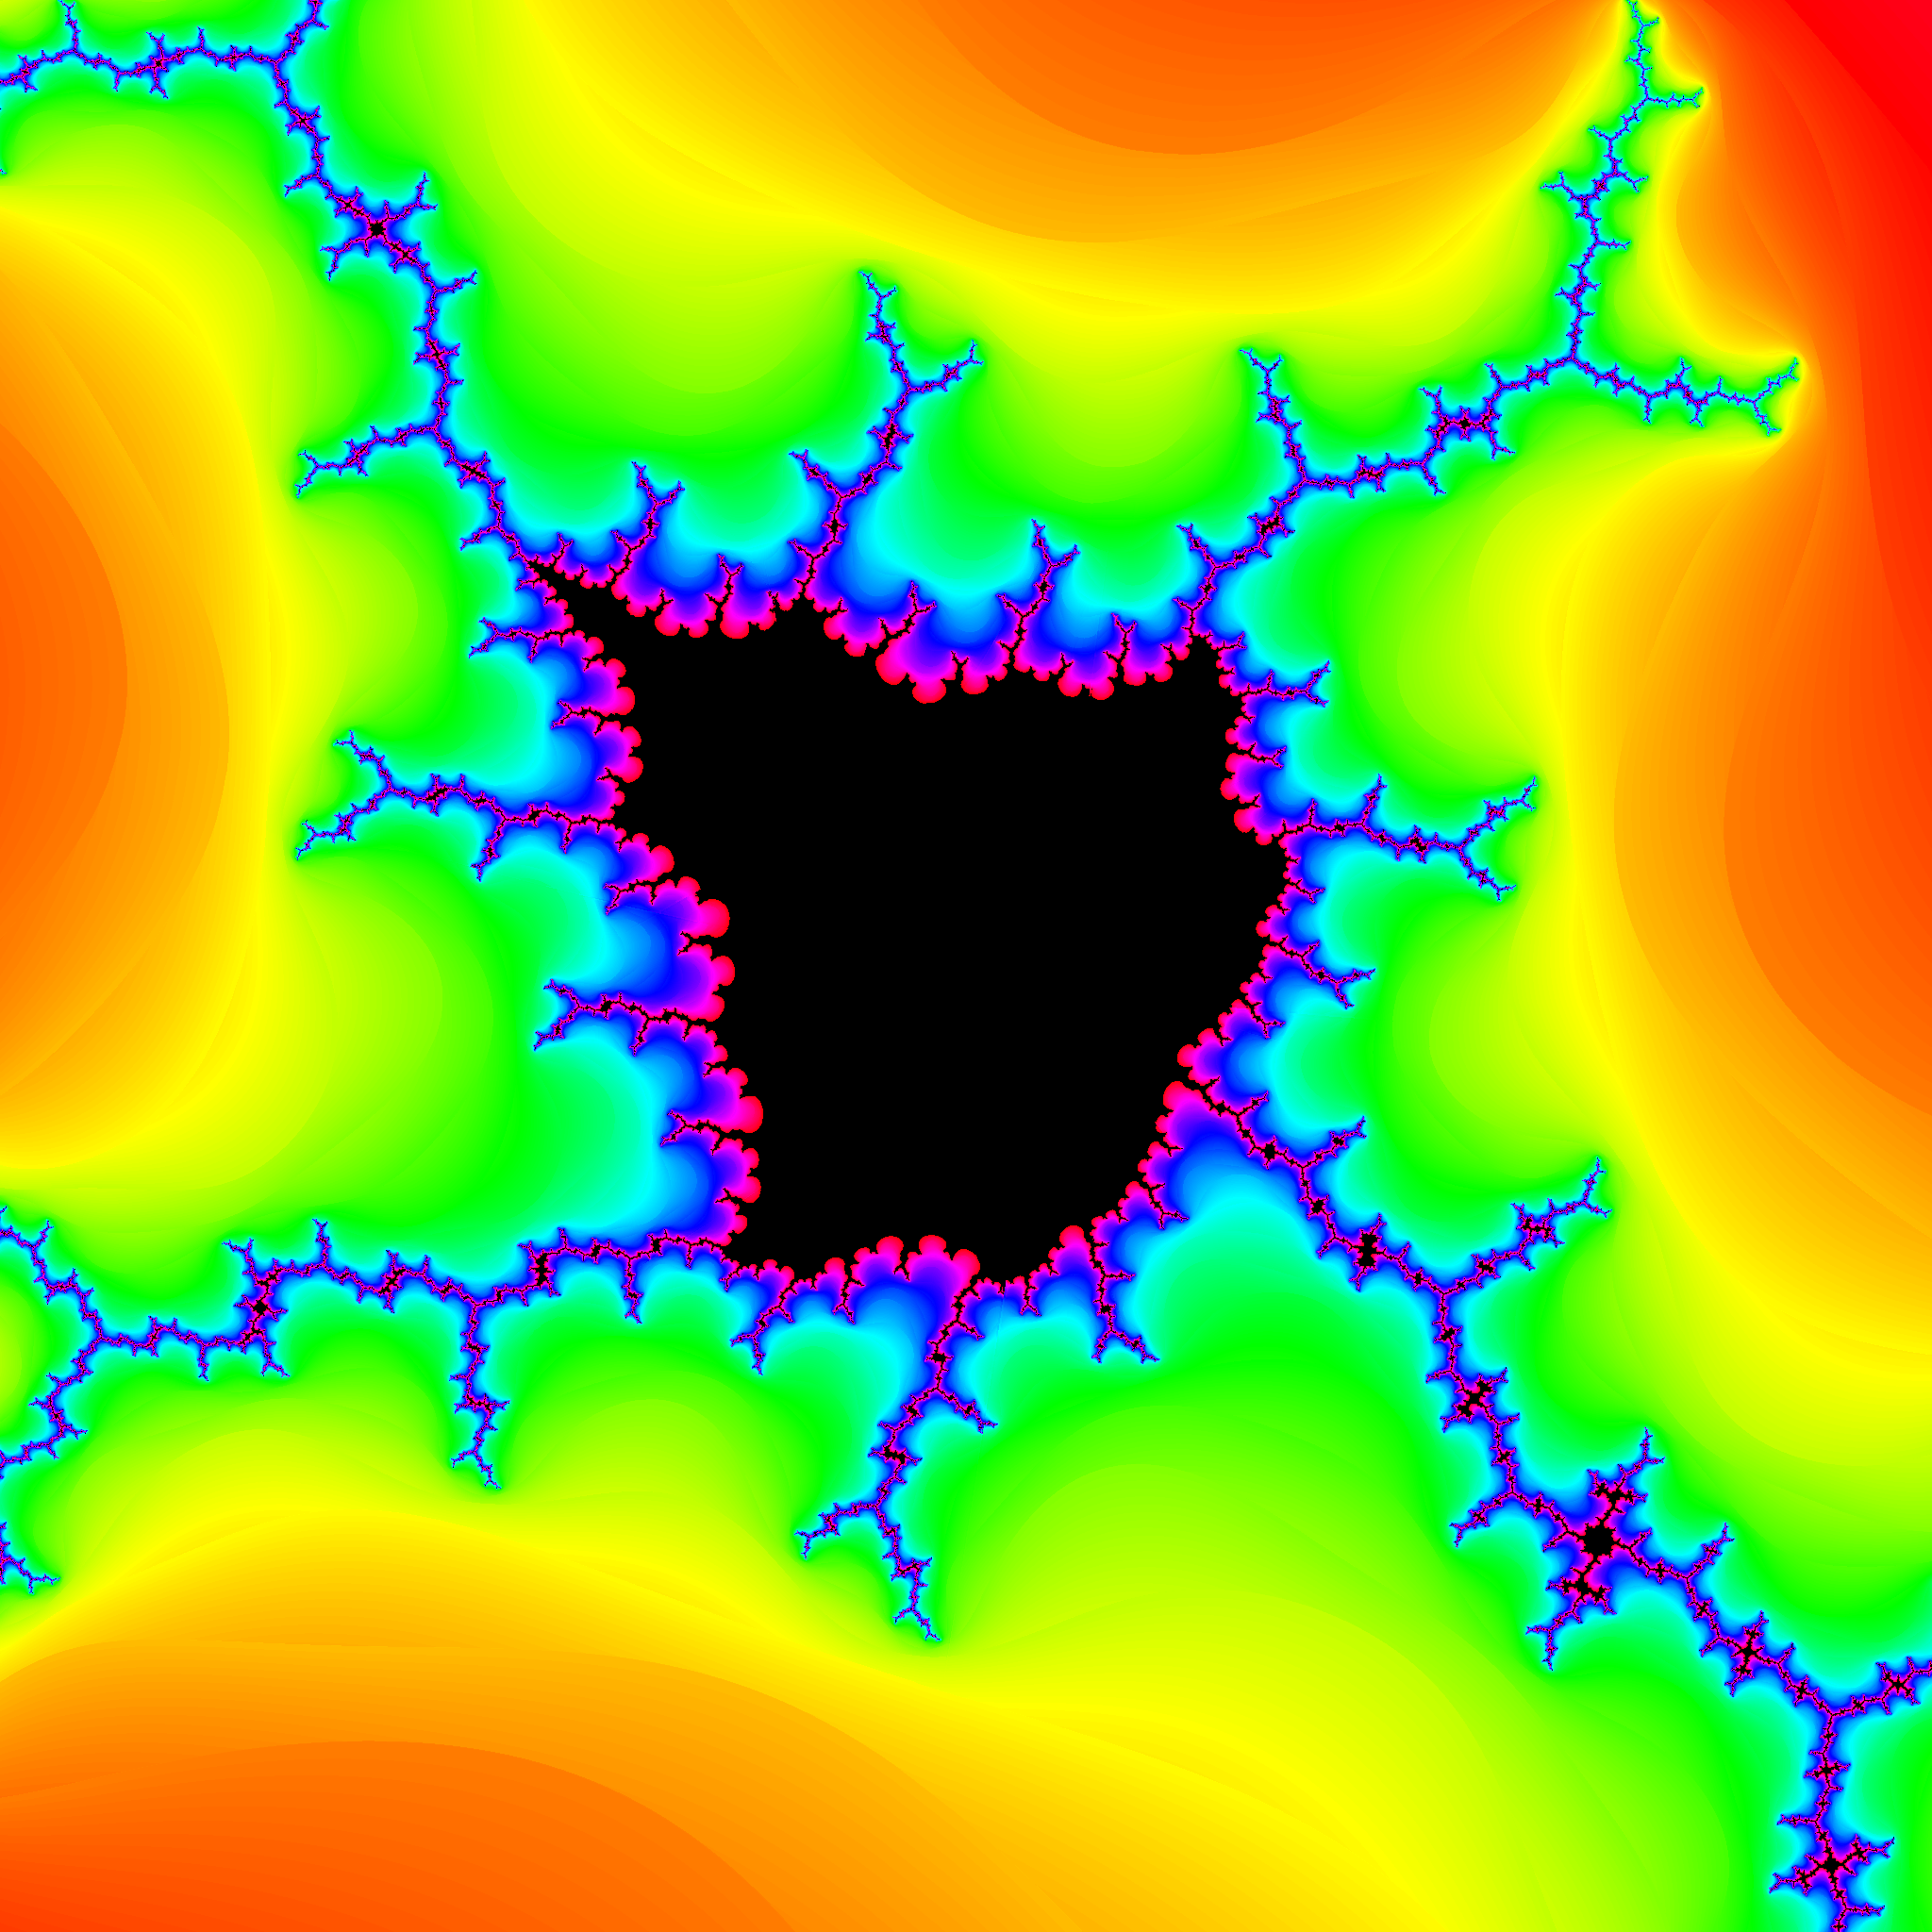
\includegraphics[width=0.45\linewidth]{images/4-starburst/mf4.png}
    \end{subfigure}
    \quad
        \begin{subfigure}[MaskedFloat<3,50>]
        \centering
        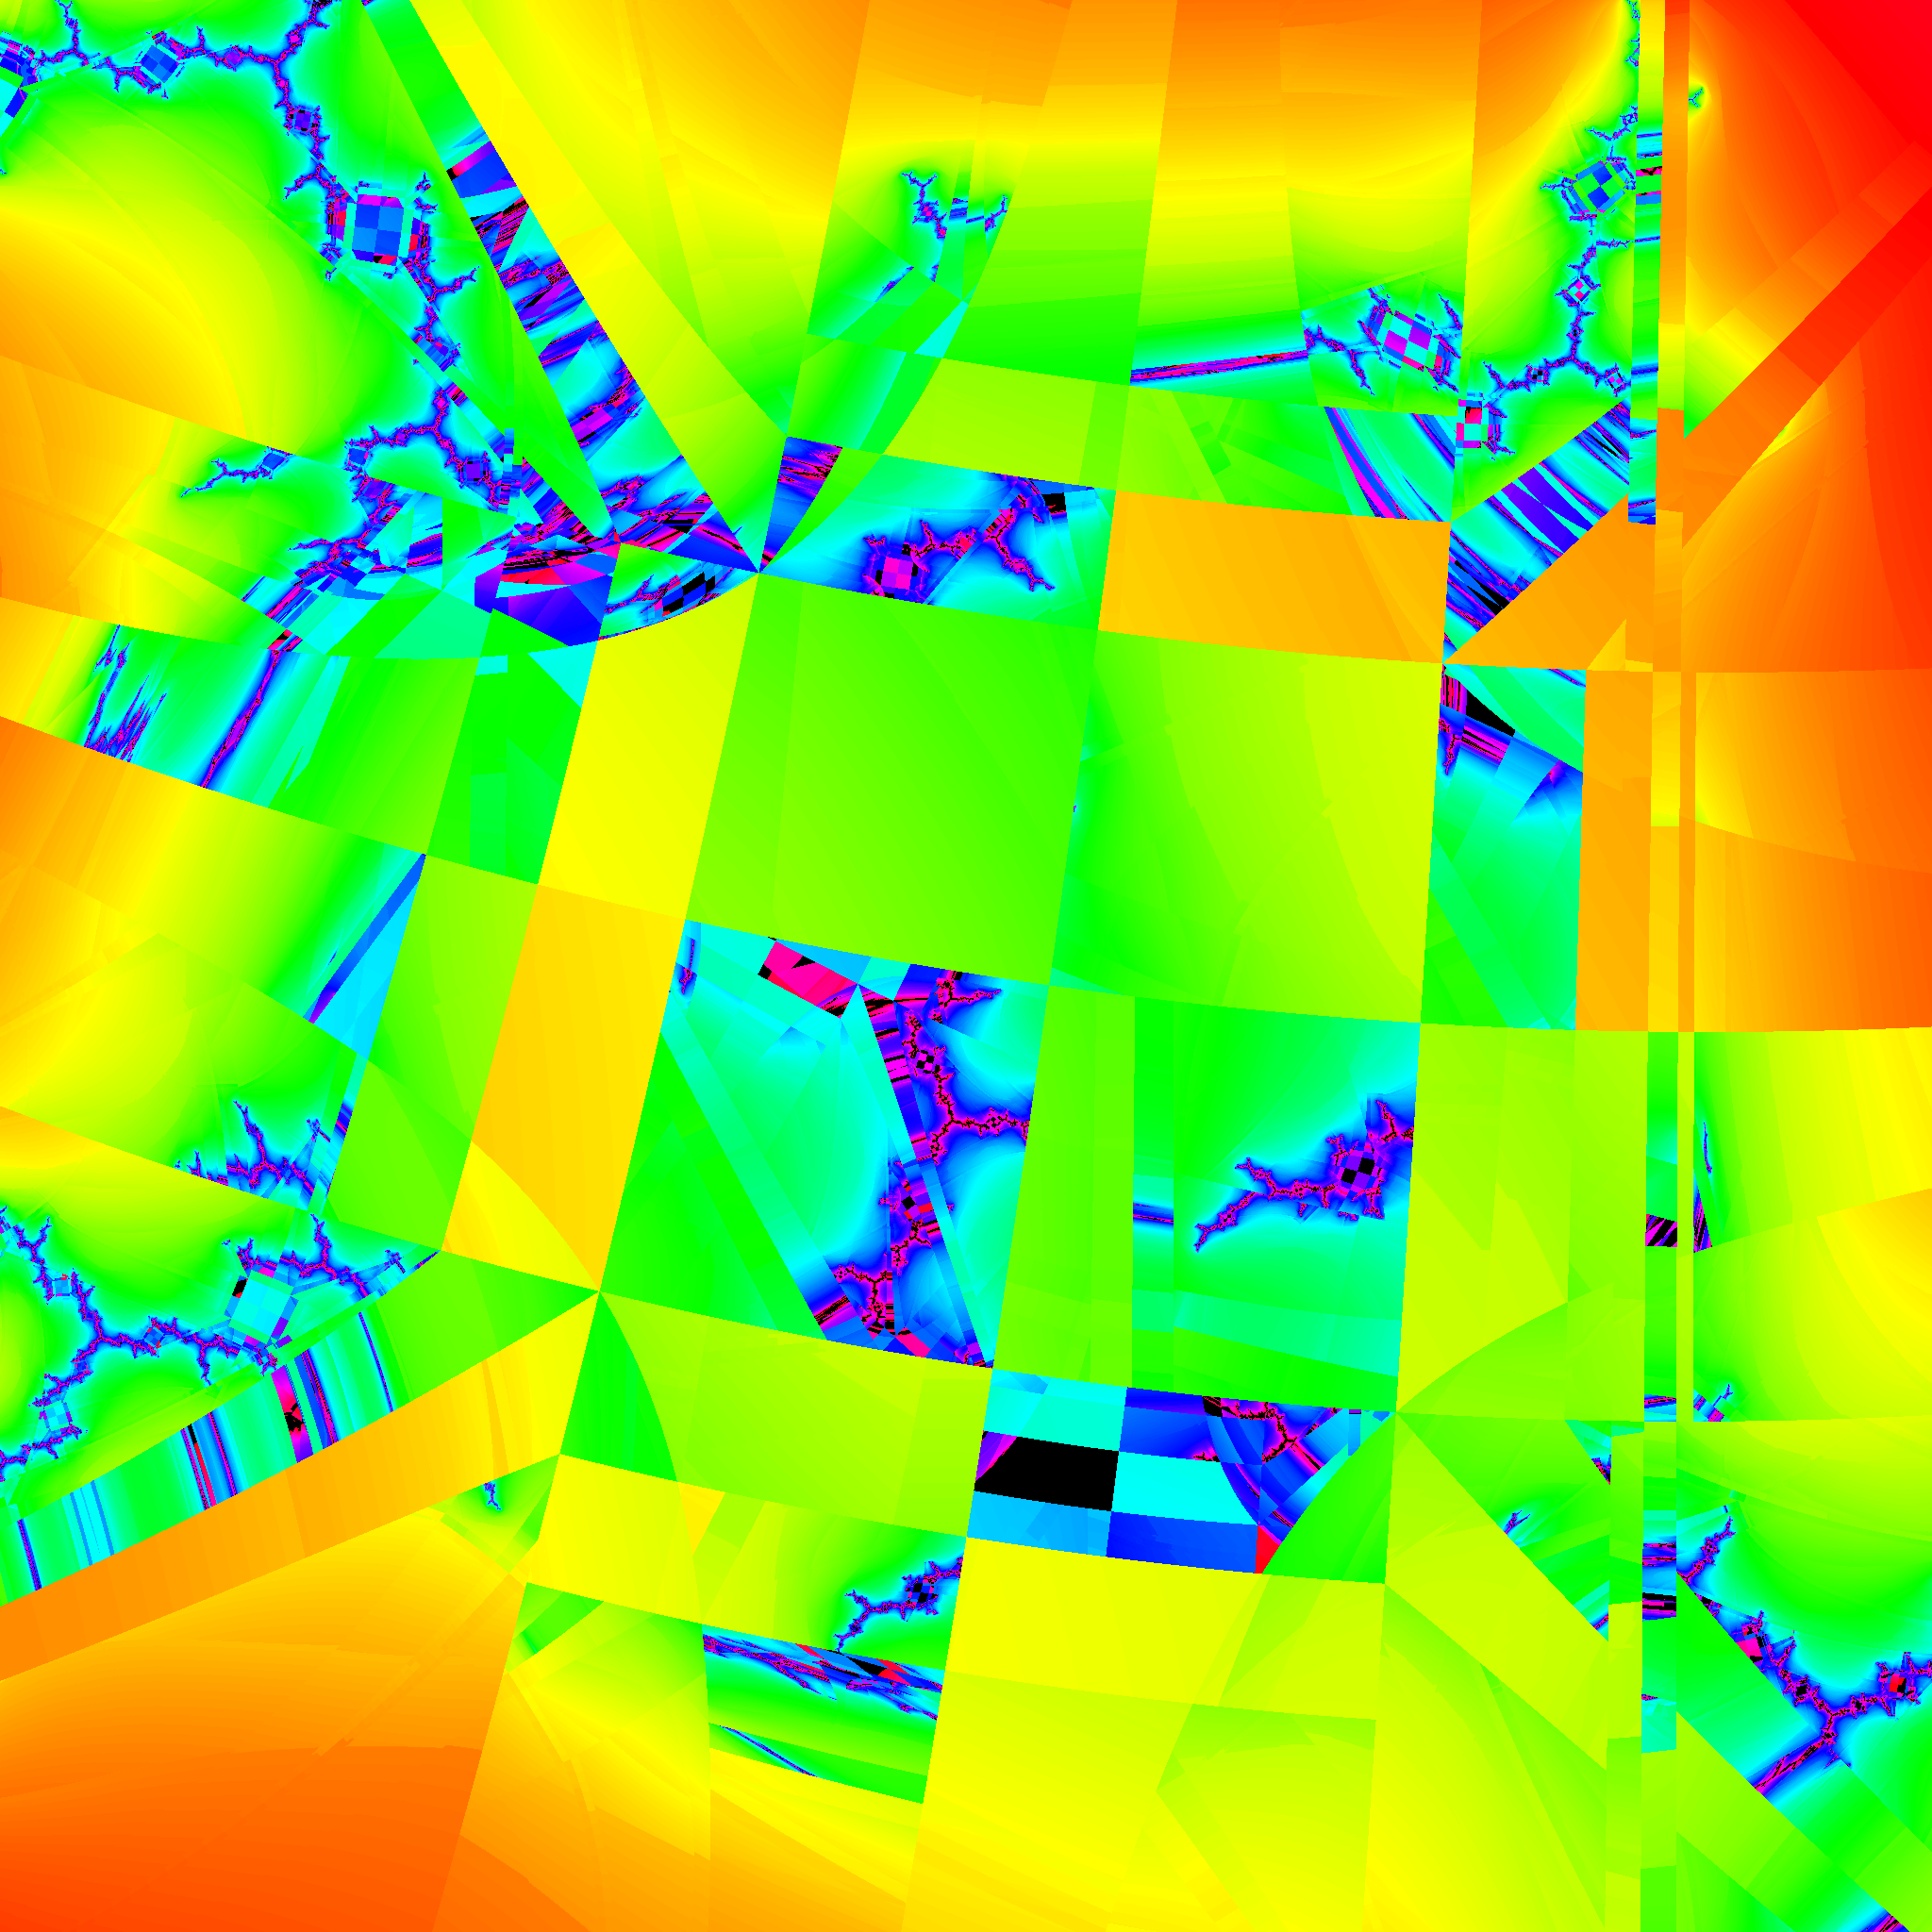
\includegraphics[width=0.45\linewidth]{images/4-starburst/mf3.png}
    \end{subfigure}
    \caption{A Mandelbrot-like region of Mandelbrot}
    \label{fig:4-hyperbole}
\end{figure}

\setcounter{subsection}{712890624}
\subsection{Hyperbolic startbursts}

One additional pattern of distortion that MaskedFloat formats demonstrate is the "hyperbolic starburst",\footnote{It's only a starburst if you imagine its shape greatly exaggerated.} so named for its appearance during an earlier (buggier)
implementation of MaskedFloat. This pattern seems to appear in Mandelbrot
near denser regions of the set e.g. repetitions of the Mandelbrot "beetle" shape.

For instance, Figure \ref{fig:4-hyperbole} shows two MaskedFloat configurations in the same range: centered on a beetle, in the lighting off of the north bulb. Note that some portions of \texttt{MaskedFloat<3,50>} mirror the fine structure of the fractal (lighting bolts), while others appear to be curvilinear.

%% /mandelbrot/?x=-3593889&y=-23416182&window=1048576&scale=22674816&res=2048&iters=32

\setcounter{subsection}{857421874}
\subsection{Errors abound?}

%% /mandelbrot/?x=-50314256&y=62360216&window=864&scale=109350000&res=512&iters=280

\begin{figure}
    \begin{subfigure}[f64]
        \centering
        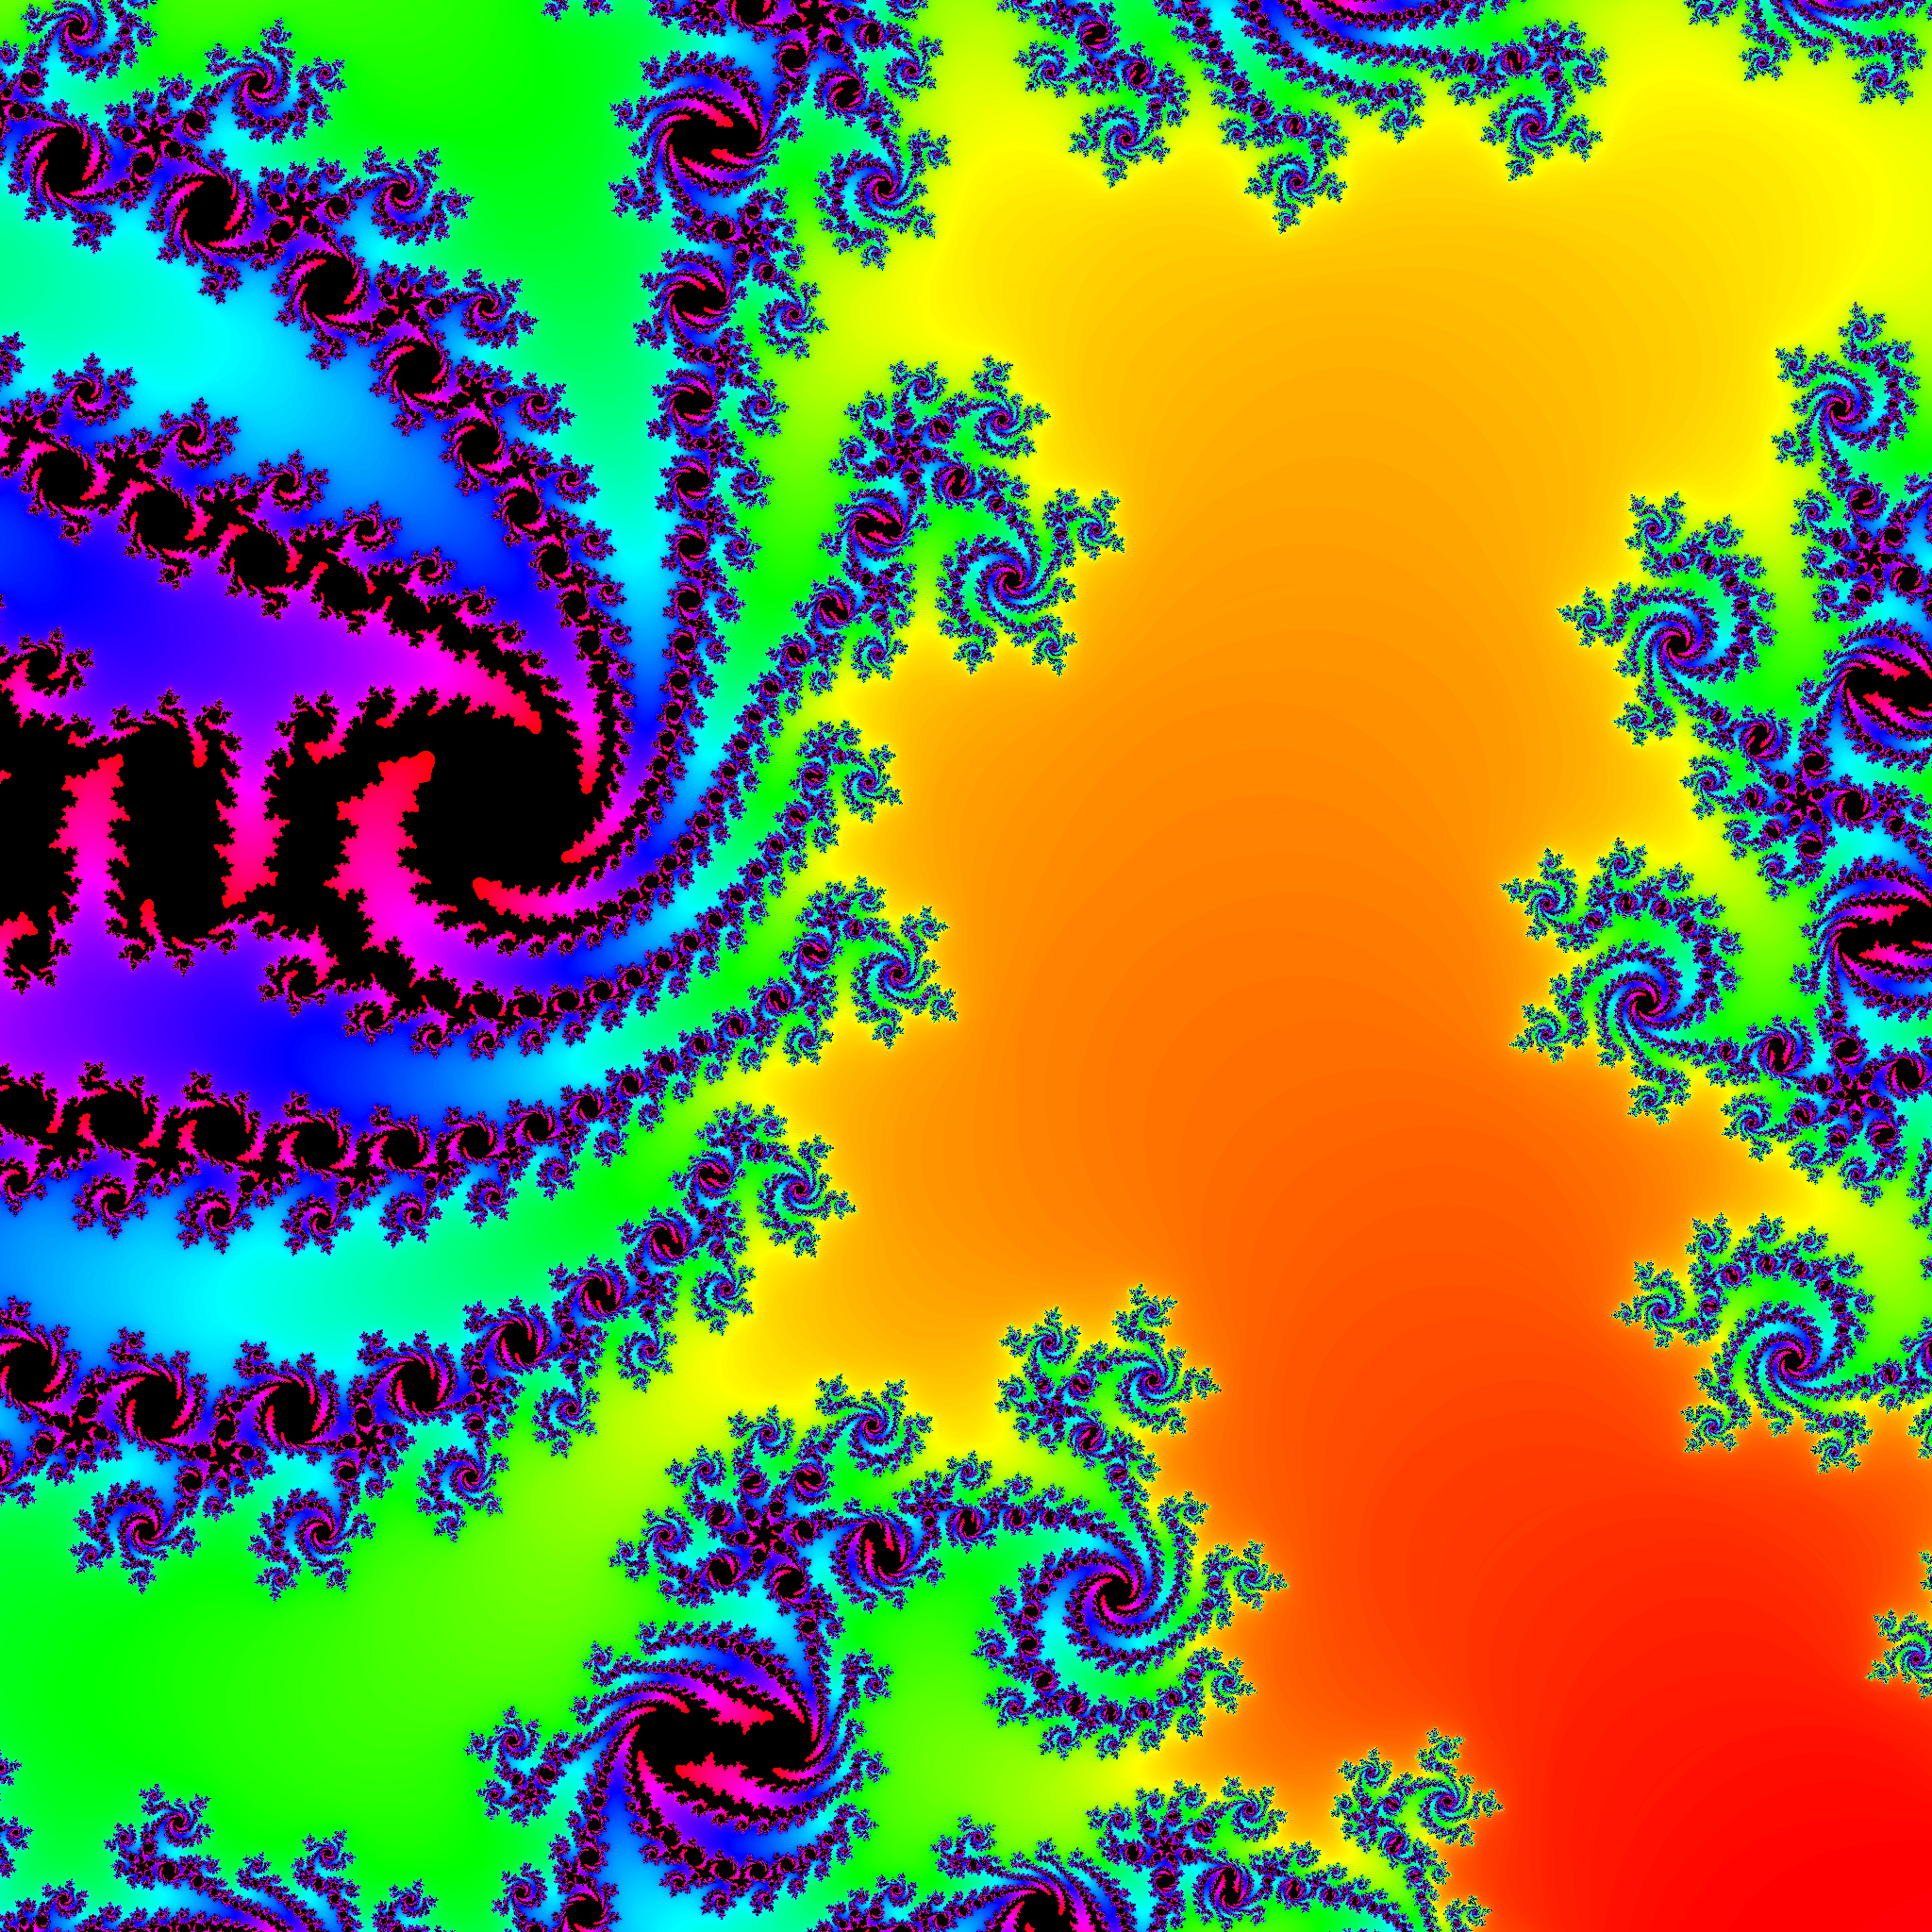
\includegraphics[width=0.45\linewidth]{images/5-uhhh/f64.png}
    \end{subfigure}
    \quad
    \begin{subfigure}[MaskedFloat<4,50>]
        \centering
        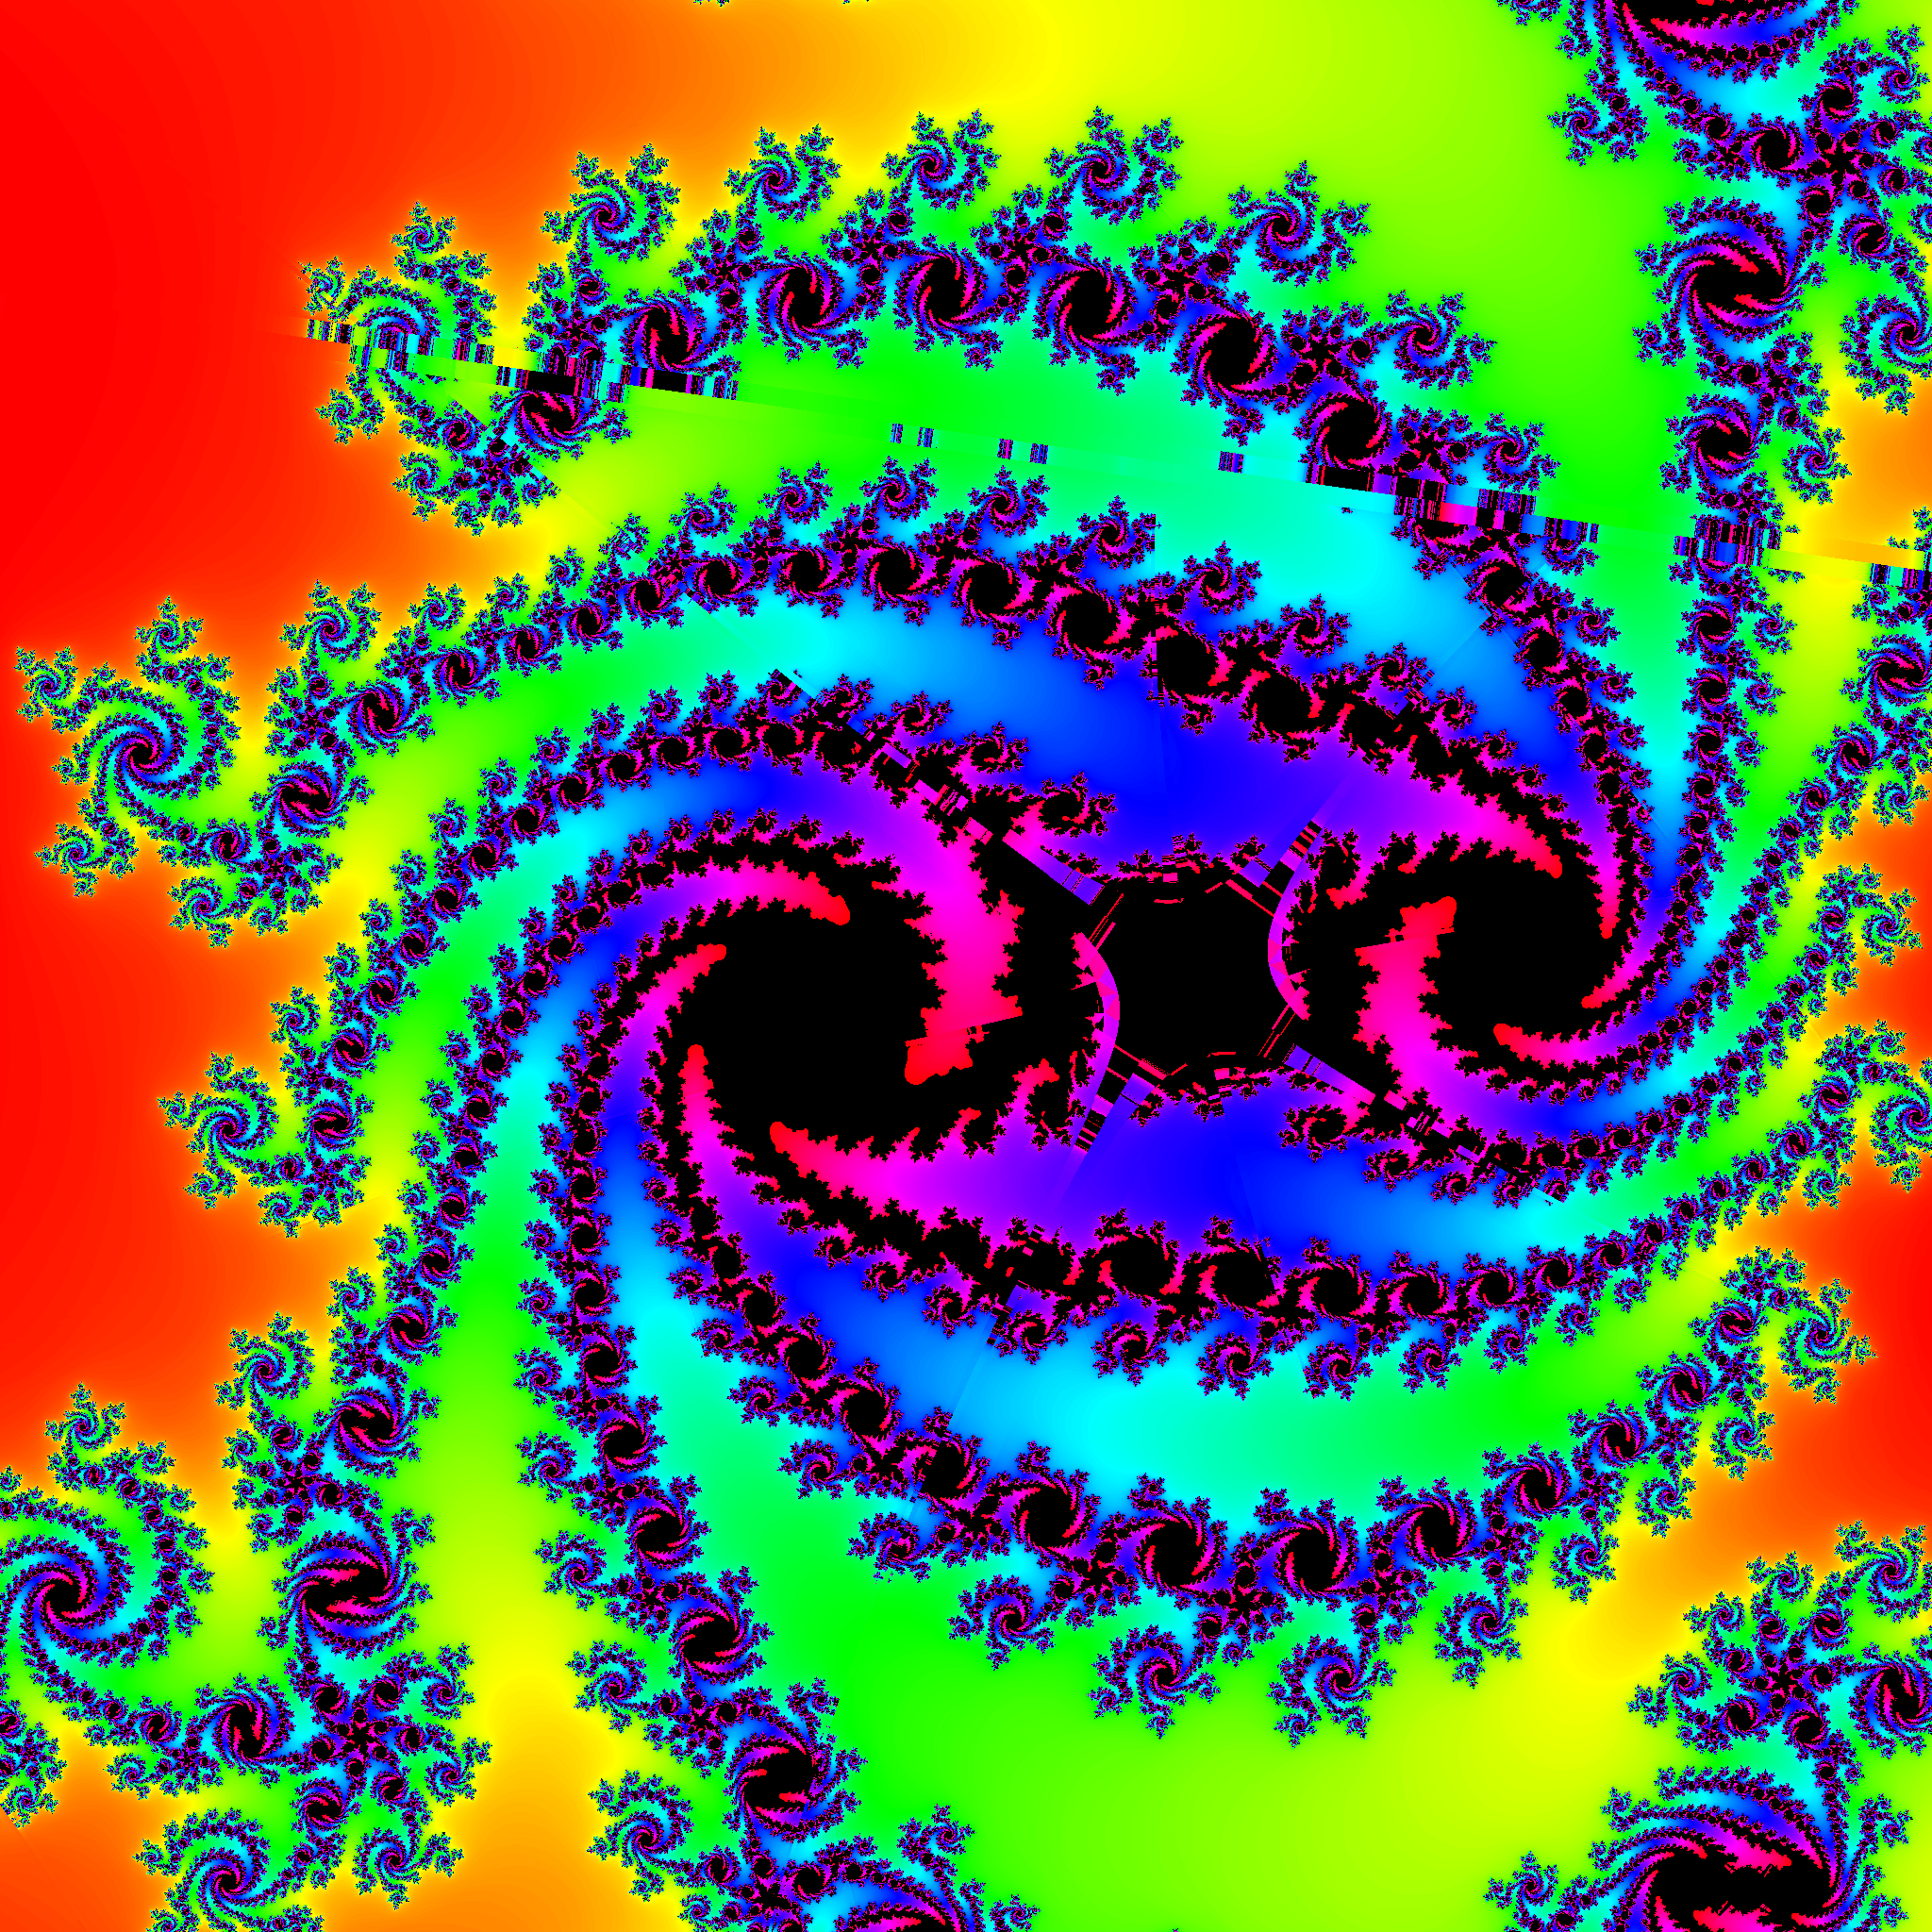
\includegraphics[width=0.45\linewidth]{images/5-uhhh/mf4.png}
    \end{subfigure}
    \quad
    \caption{Computational errors in MaskedFloat?}
    \label{fig:5-uhhh}
\end{figure}

Figure \ref{fig:5-uhhh} shows something even odder: an apparent structural difference between \texttt{f64} and a MaskedFloat format. Whether this points to an offset
error in the format, or another issue, we leave for future investigators.

\setcounter{section}{6}
\section{Assessment and future work}

We unequivocally recommend the MaskedFloat family of numeric formats for making weird-looking fractal art, and whatever format(s) your hardware supports for everything else.

The authors only explored the Newton fractal on the Wikipedia example polynomial $p(z) = z^3-1$. It's possible other Newton
fractals would lead to more cool distortion. As the core operation in Newton's fractal is very similar to the 
core operation in machine learning's gradient descent calculation, there's probably an ML-adjacent paper one could 
shovel out about this, if you want big-corp funding.

% \section{Coda: Precise Section Numbering}
% When typesetting this paper, we attempted to number the first two subsections
% 1.33333337306976318359375 and 1.66666662693023681640625, accurately representing
% their position within the section up to the precision of an \texttt{f32}.
% However, our typesetting software only permits section values up to
% 2147483647; this limits our section numbers to 9 fractional bits in a fixed-point format.

%   \section{Prebuilt sections}
%   \subsection{Do Not Remove Boilerplate Code}
%   The TEX document includes code to generate sections such as the the copyright block. Do not remove these. Authors of accepted papers will receive sections of code to replace these and customise the final paper accordingly.
    
%   Pay attention to the code comments about author information and add/remove authors as necessary; there must be at least one author. It is desirable that all/most authors have an ORCID ID as this is replacing the need for explicit emails (that my change as researcher move around. If an ORCID is supplied that author's name is made the anchor text of a web link to their ORCID page. 
    
%   Macro codes are offered (\texttt{e.g. authornote}) which may be used as well as indicating the corresponding author(s) for communication during publication.
    
%   \subsection{General points on ACM papers}
%   See the file `sample-sigconf.pdf' provided with this template set. It explains the basics of a number of structural features.

%    Newer users of \LaTeX\ should take care to understand \LaTeX's special characters that need explicit escaping. Also be aware that typographic quotes and en-dash/em-dash hyphens are not used literally in TEX documents but are indicated with macros.
    
%   Overleaf has extensive documentation covering how to indicate typographic elements in \LaTeX code.
    
%   \subsubsection{A Third-level Heading} 
%   Note that level-three headings are inset into the beginning in the first paragraph of that section, regardless of line breaks in the source document.
    
%   Sections at all three levels are auto-numbered, so these do not need to be numbered in your text.


%%
%% The acknowledgments section is defined using the "acks" environment
%% (and NOT an unnumbered section). This ensures the proper
%% identification of the section in the article metadata, and the
%% consistent spelling of the heading.
\begin{acks}
Thanks to M+T for leaving Stephen enough sleep to work on this. Thanks to Q for supporting Charles while working on this.

Well, we say "work"...
\end{acks}

%%
%% The next two lines define the bibliography style to be used, and
%% the bibliography file.
\bibliographystyle{ACM-Reference-Format}
\bibliography{references.bib}

\appendix
\section*{APPENDIX}
\section{Artifacts}

Just go to Github: \url{https://github.com/cceckman/fractal-farlands}


%%
\end{document}
\endinput
%%
%% End of file `main.tex'.
